

% arkiv figurer

\begin{figure}[H]
    \centering
    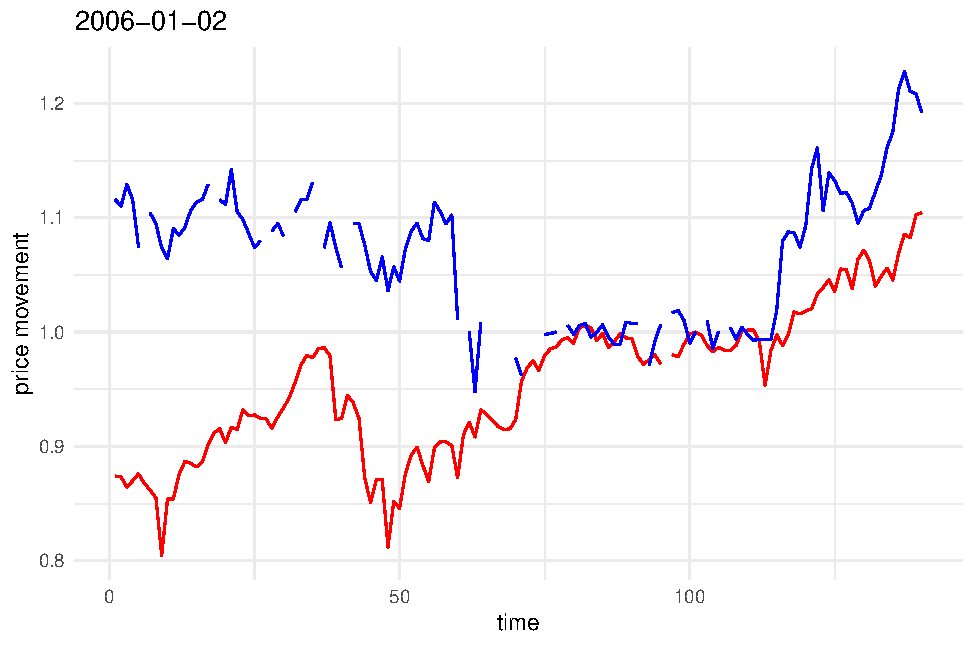
\includegraphics{plots/plot_for_2006-01-02.pdf}
    \caption{Caption}
    \label{fig:enter-label}
\end{figure}

\begin{figure}[H]
    \centering
    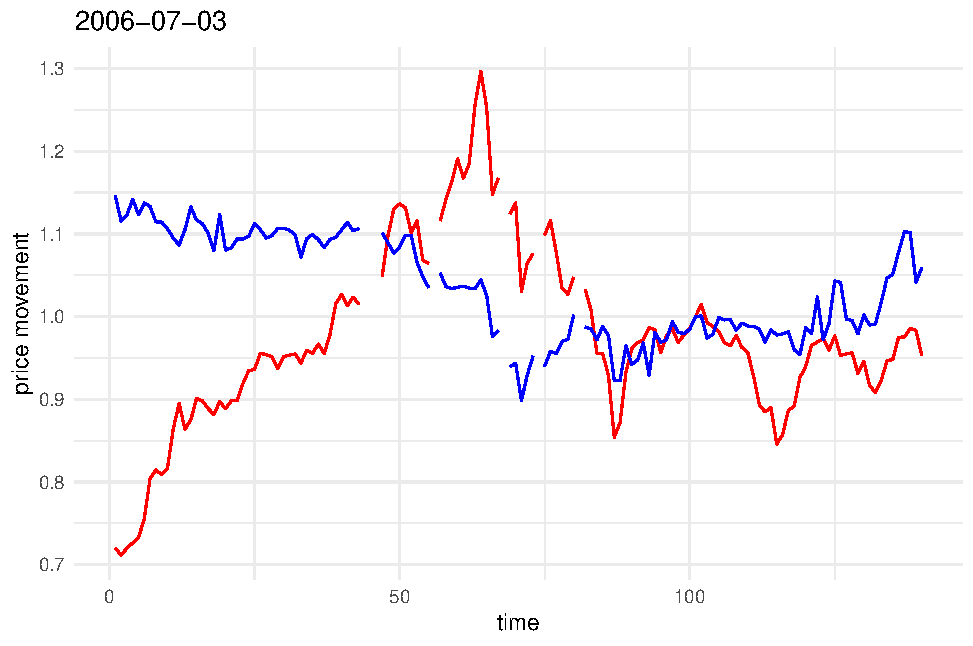
\includegraphics{plots/plot_for_2006-07-03.pdf}
    \caption{Caption}
    \label{fig:enter-label}
\end{figure}

\begin{figure}[H]
    \centering
    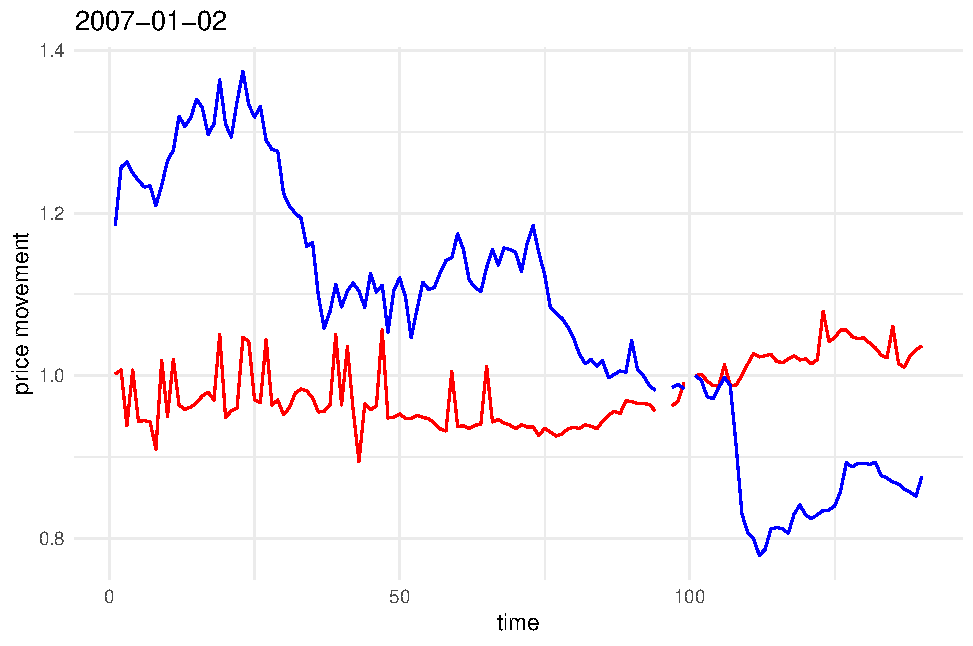
\includegraphics{plots/plot_for_2007-01-02.pdf}
    \caption{Caption}
    \label{fig:enter-label}
\end{figure}

\begin{figure}[H]
    \centering
    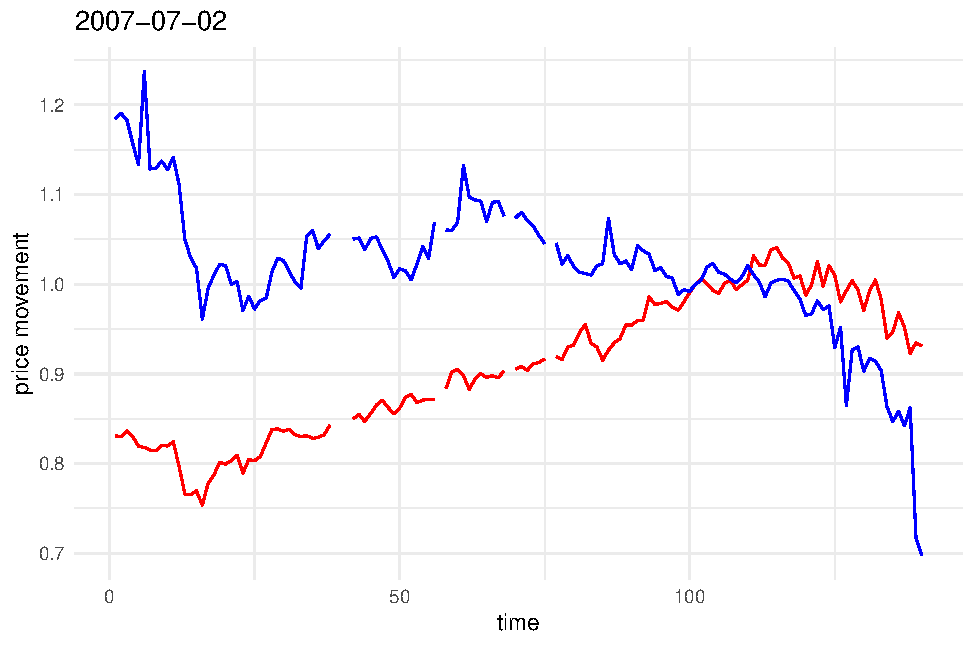
\includegraphics{plots/plot_for_2007-07-02.pdf}
    \caption{Caption}
    \label{fig:enter-label}
\end{figure}

\begin{figure}[H]
    \centering
    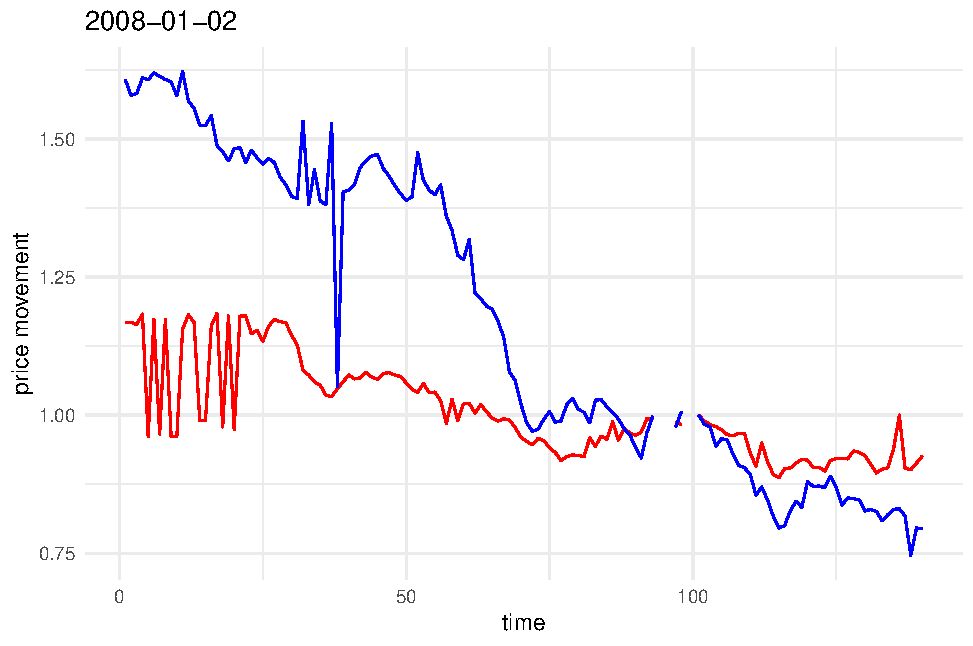
\includegraphics{plots/plot_for_2008-01-02.pdf}
    \caption{Caption}
    \label{fig:enter-label}
\end{figure}

\begin{figure}[H]
    \centering
    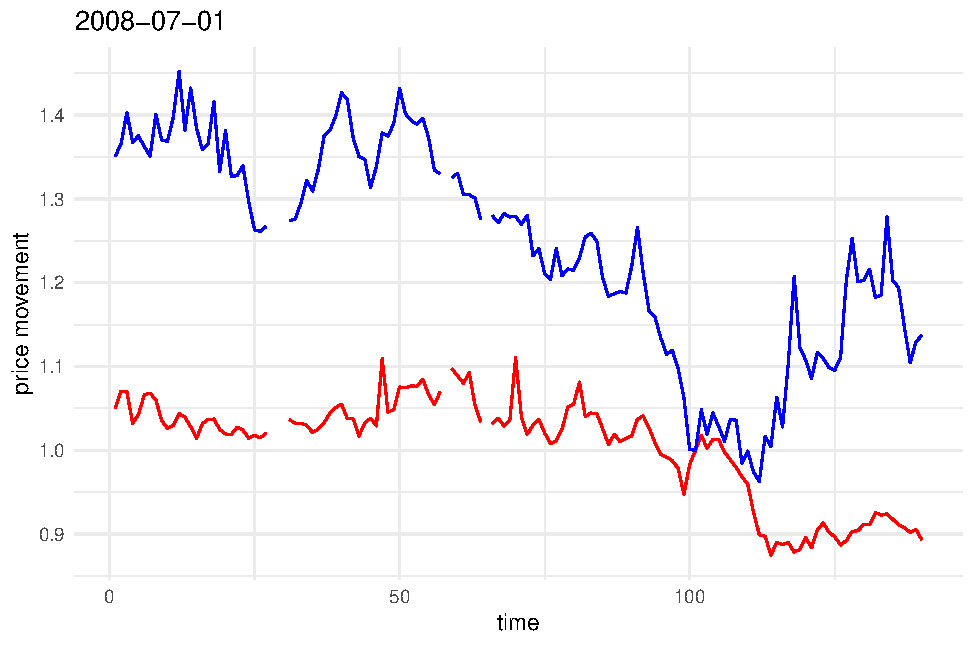
\includegraphics{plots/plot_for_2008-07-01.pdf}
    \caption{Caption}
    \label{fig:enter-label}
\end{figure}

\begin{figure}[H]
    \centering
    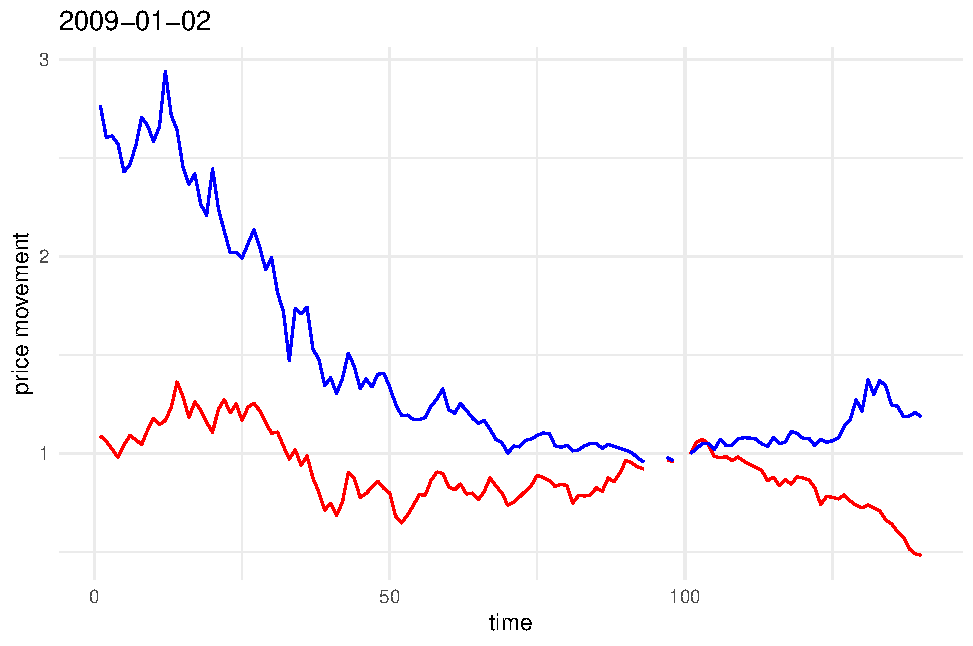
\includegraphics{plots/plot_for_2009-01-02.pdf}
    \caption{Caption}
    \label{fig:enter-label}
\end{figure}

\begin{figure}[H]
    \centering
    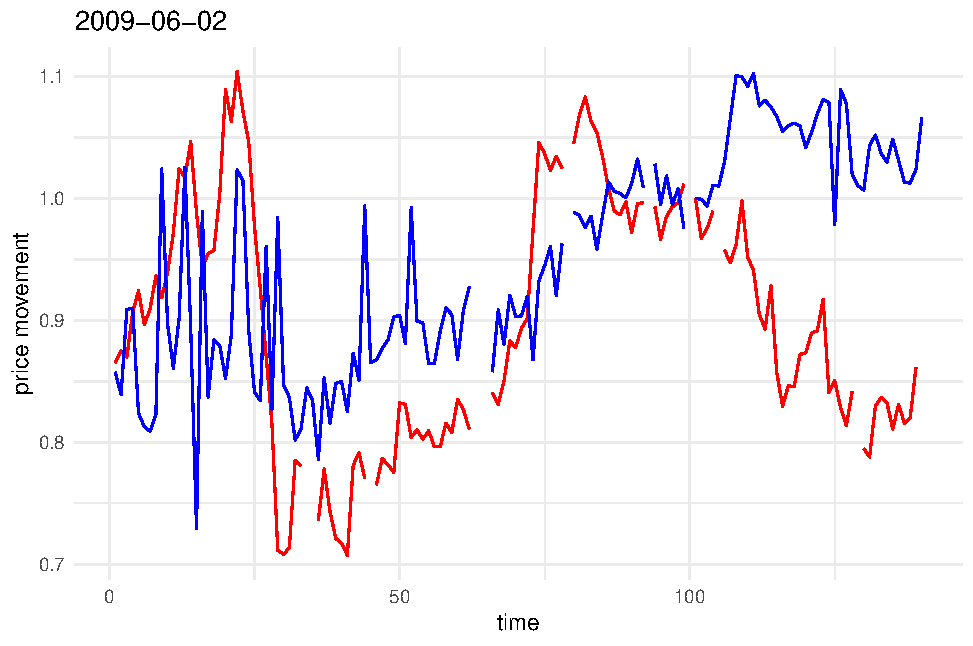
\includegraphics{plots/plot_for_2009-06-02.pdf}
    \caption{Caption}
    \label{fig:enter-label}
\end{figure}

\begin{figure}[H]
    \centering
    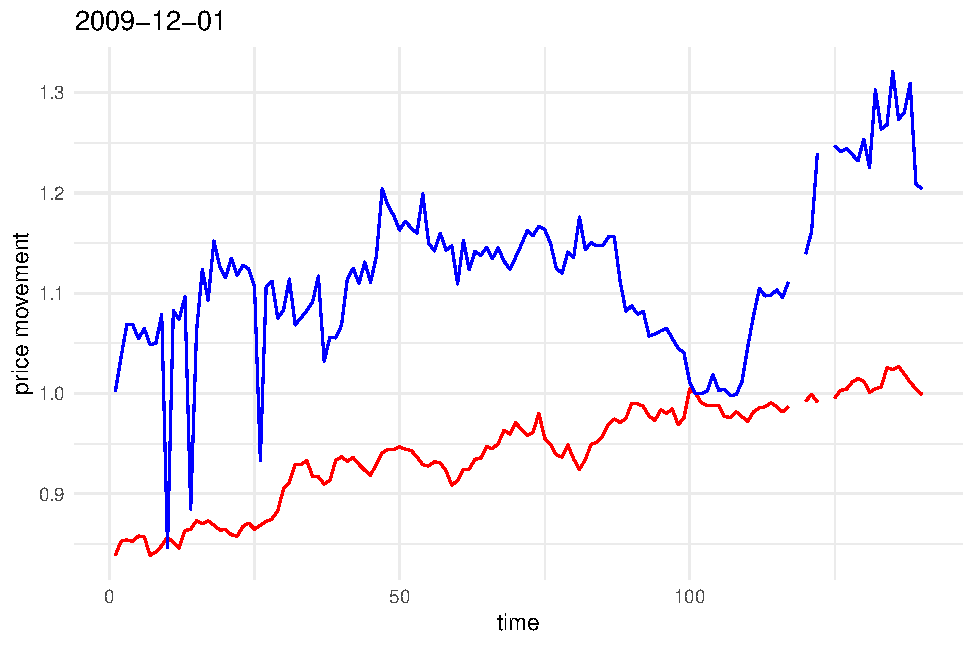
\includegraphics{plots/plot_for_2009-12-01.pdf}
    \caption{Caption}
    \label{fig:enter-label}
\end{figure}

\begin{figure}[H]
    \centering
    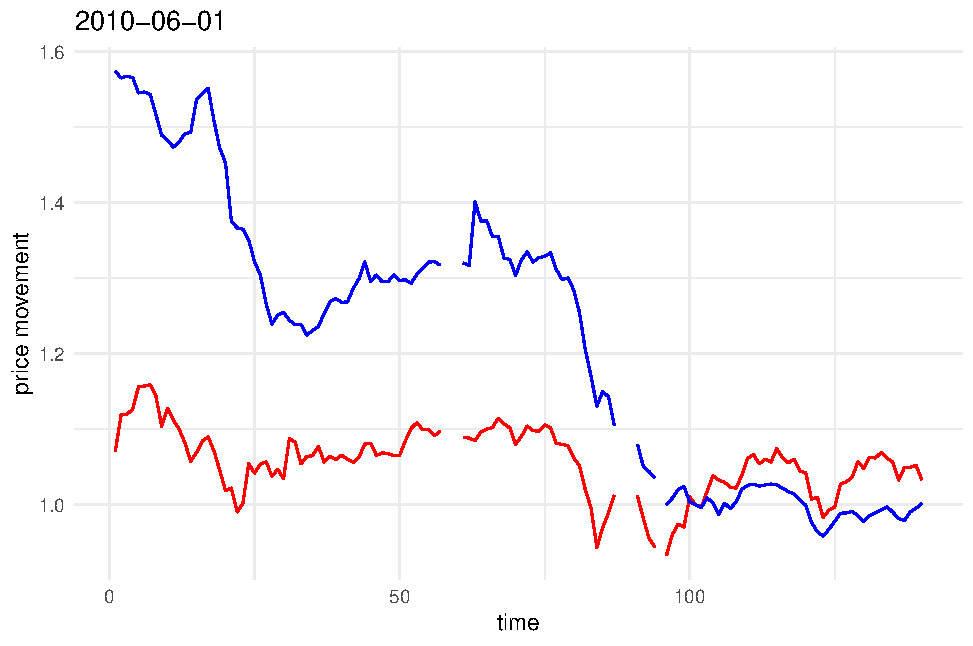
\includegraphics{plots/plot_for_2010-06-01.pdf}
    \caption{Caption}
    \label{fig:enter-label}
\end{figure}

\begin{figure}[H]
    \centering
    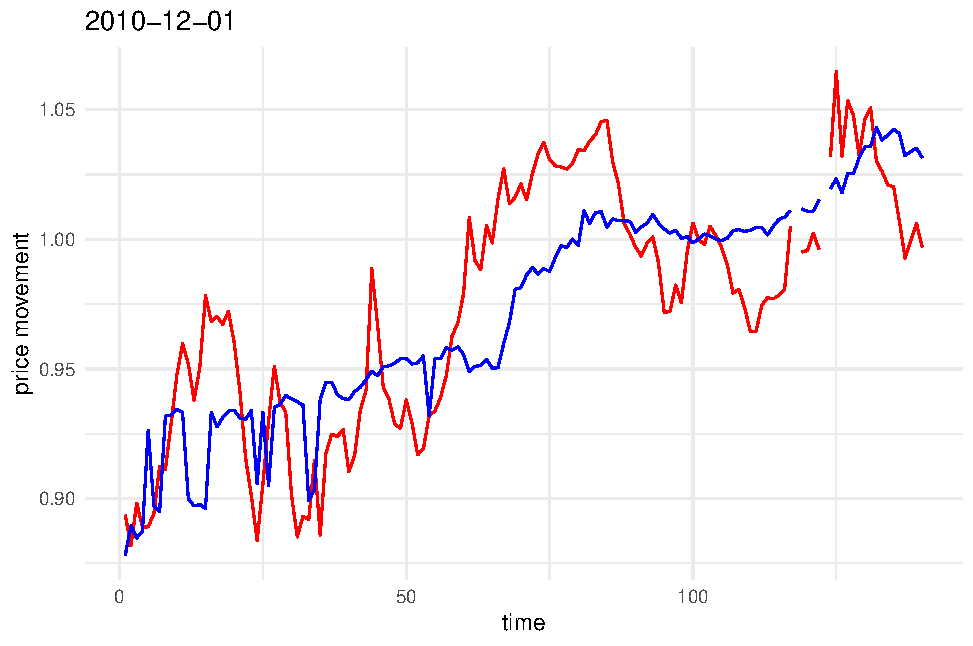
\includegraphics{plots/plot_for_2010-12-01.pdf}
    \caption{Caption}
    \label{fig:enter-label}
\end{figure}

\begin{figure}[H]
    \centering
    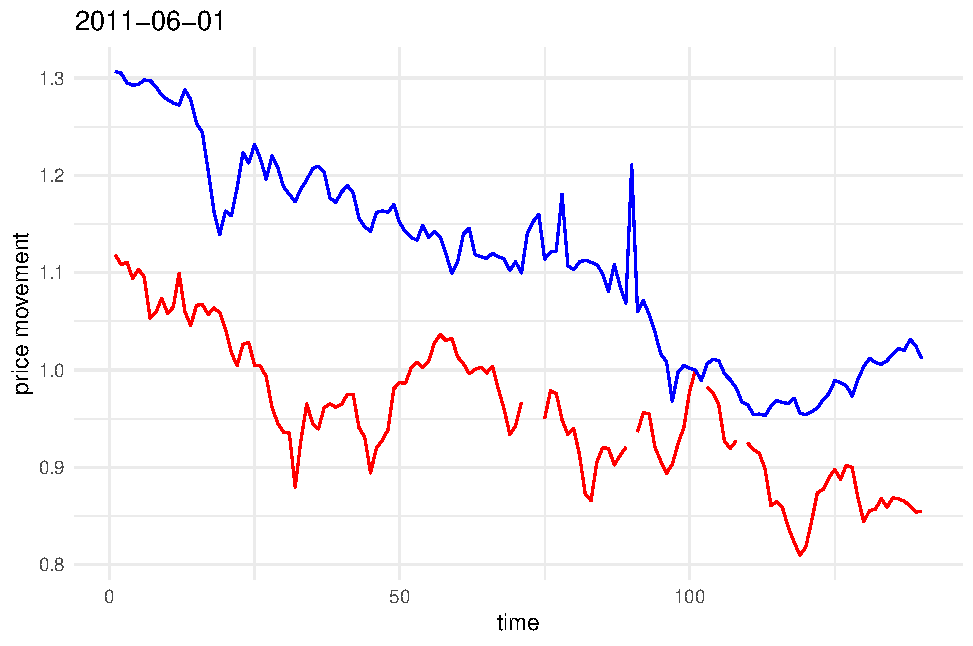
\includegraphics{plots/plot_for_2011-06-01.pdf}
    \caption{Caption}
    \label{fig:enter-label}
\end{figure}

\begin{figure}[H]
    \centering
    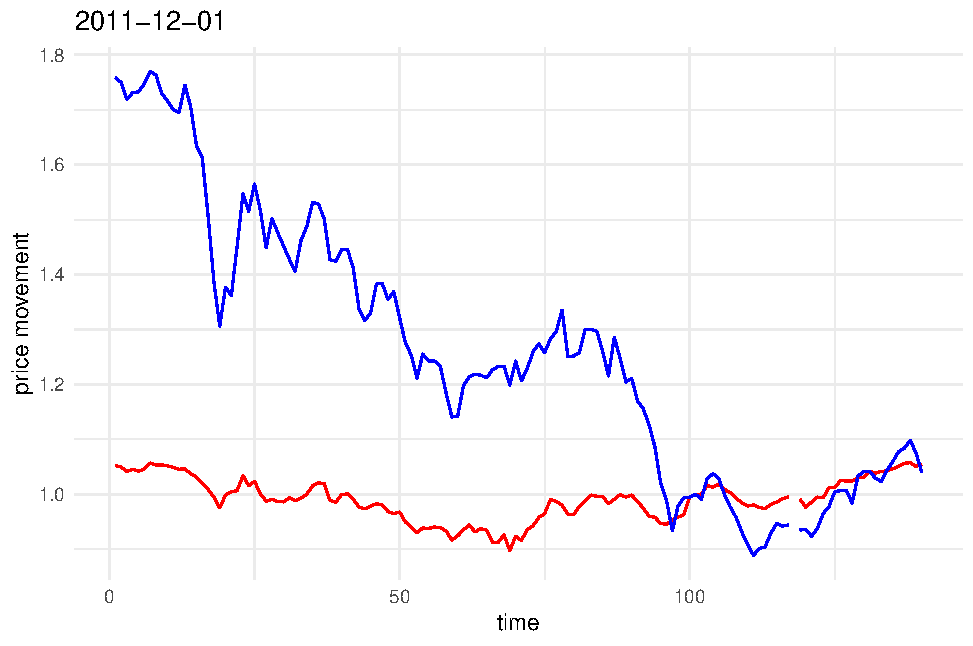
\includegraphics{plots/plot_for_2011-12-01.pdf}
    \caption{Caption}
    \label{fig:enter-label}
\end{figure}

\begin{figure}[H]
    \centering
    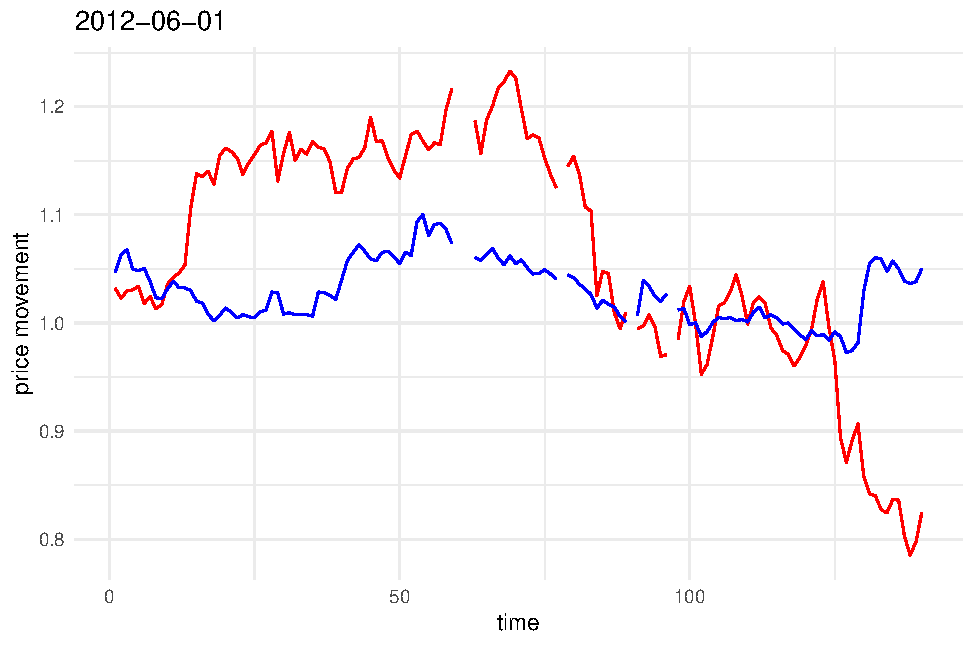
\includegraphics{plots/plot_for_2012-06-01.pdf}
    \caption{Caption}
    \label{fig:enter-label}
\end{figure}

\begin{figure}[H]
    \centering
    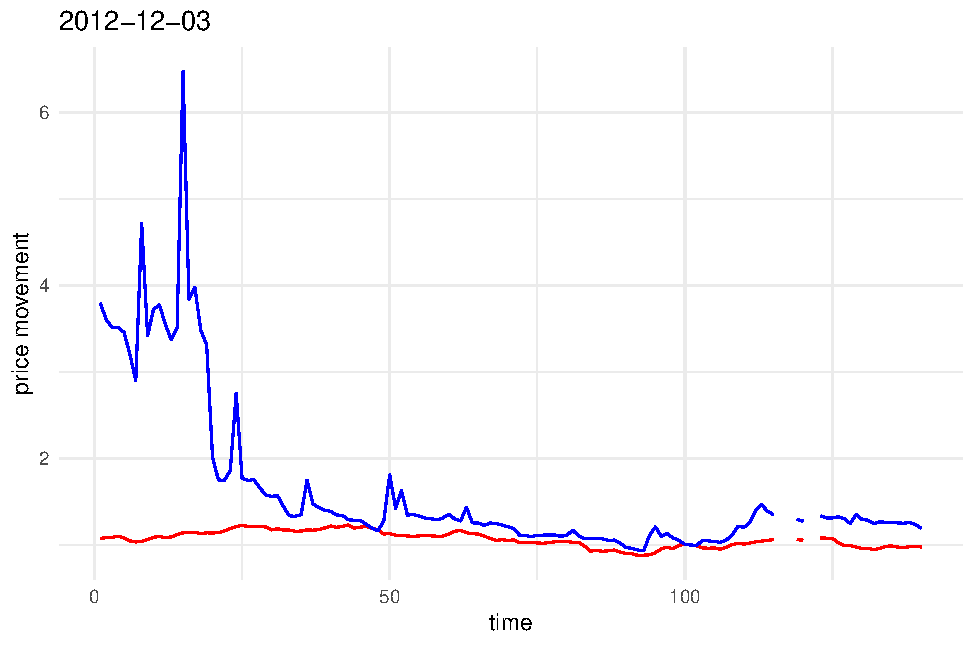
\includegraphics{plots/plot_for_2012-12-03.pdf}
    \caption{Caption}
    \label{fig:enter-label}
\end{figure}

\begin{figure}[H]
    \centering
    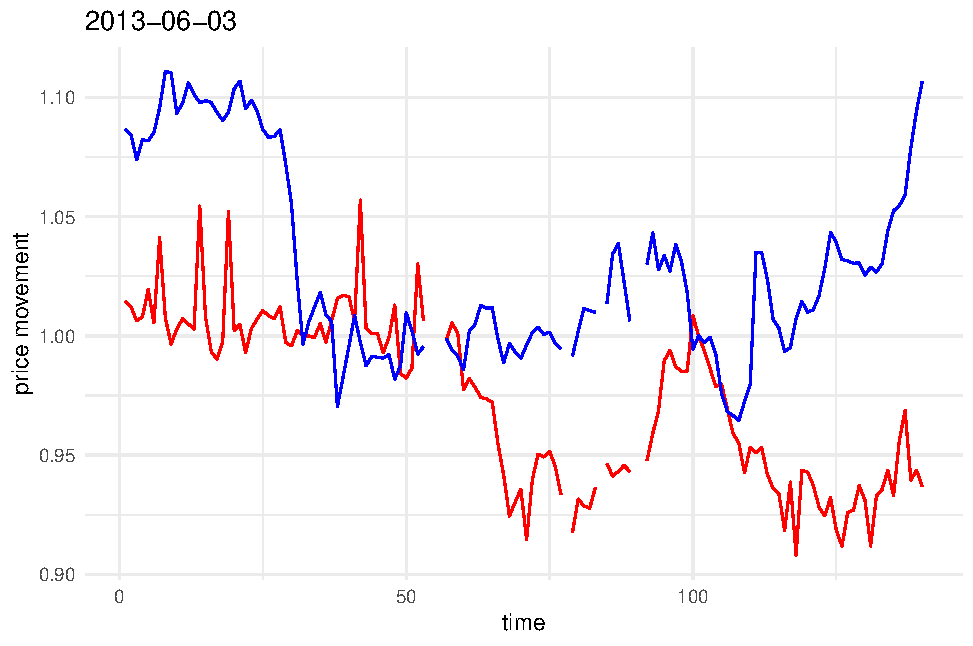
\includegraphics{plots/plot_for_2013-06-03.pdf}
    \caption{Caption}
    \label{fig:enter-label}
\end{figure}

\begin{figure}[H]
    \centering
    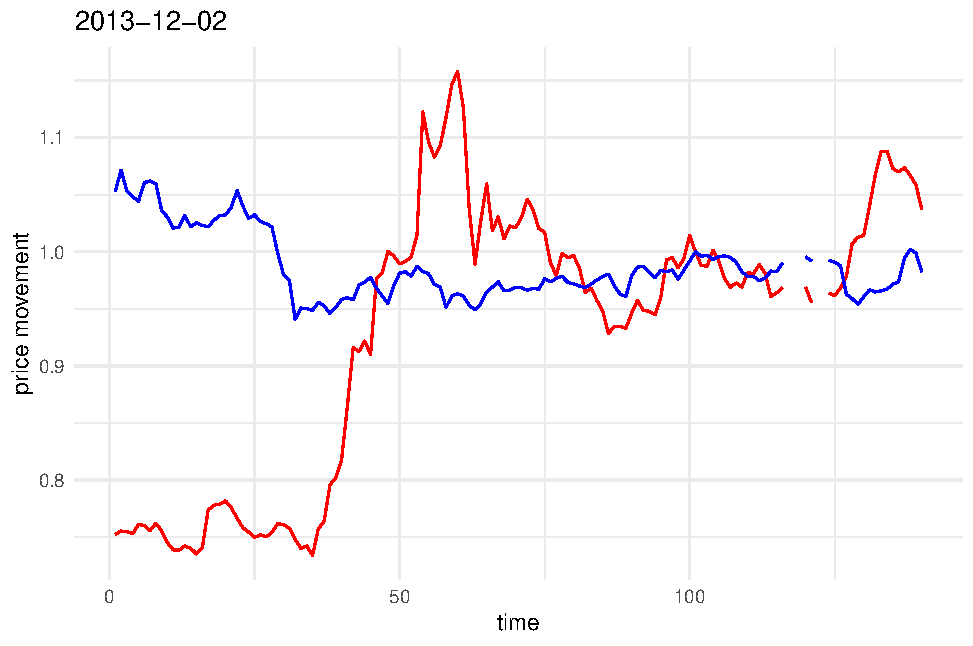
\includegraphics{plots/plot_for_2013-12-02.pdf}
    \caption{Caption}
    \label{fig:enter-label}
\end{figure}

\begin{figure}[H]
    \centering
    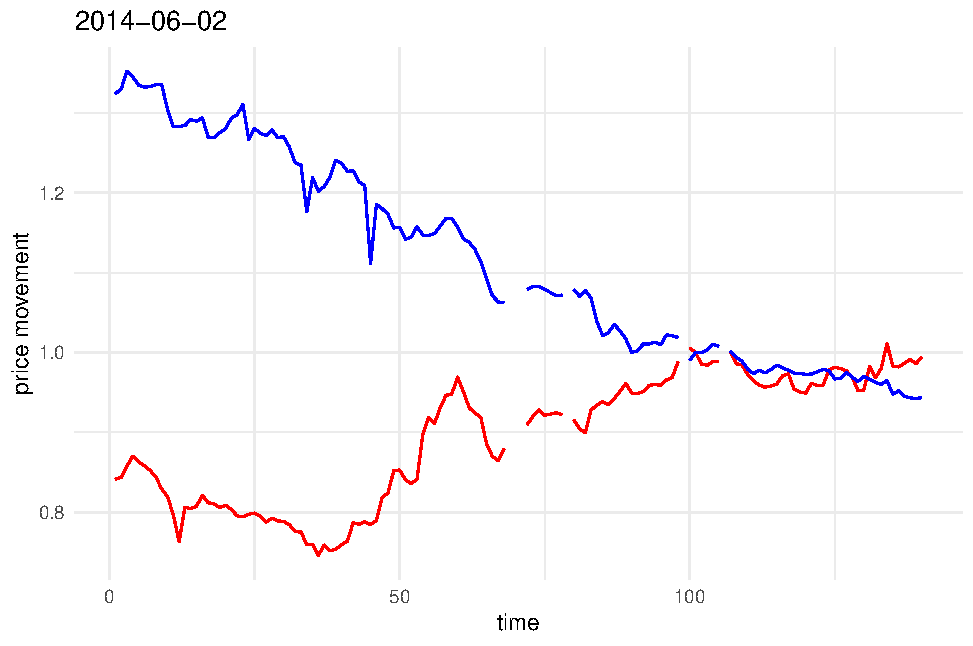
\includegraphics{plots/plot_for_2014-06-02.pdf}
    \caption{Caption}
    \label{fig:enter-label}
\end{figure}

\begin{figure}[H]
    \centering
    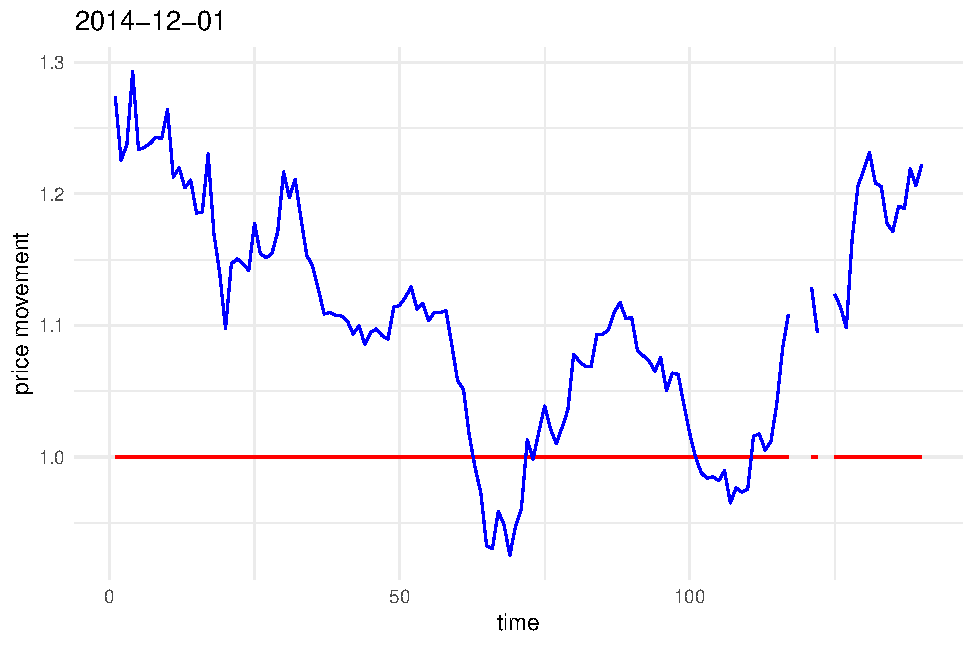
\includegraphics{plots/plot_for_2014-12-01.pdf}
    \caption{Caption}
    \label{fig:enter-label}
\end{figure}

\begin{figure}[H]
    \centering
    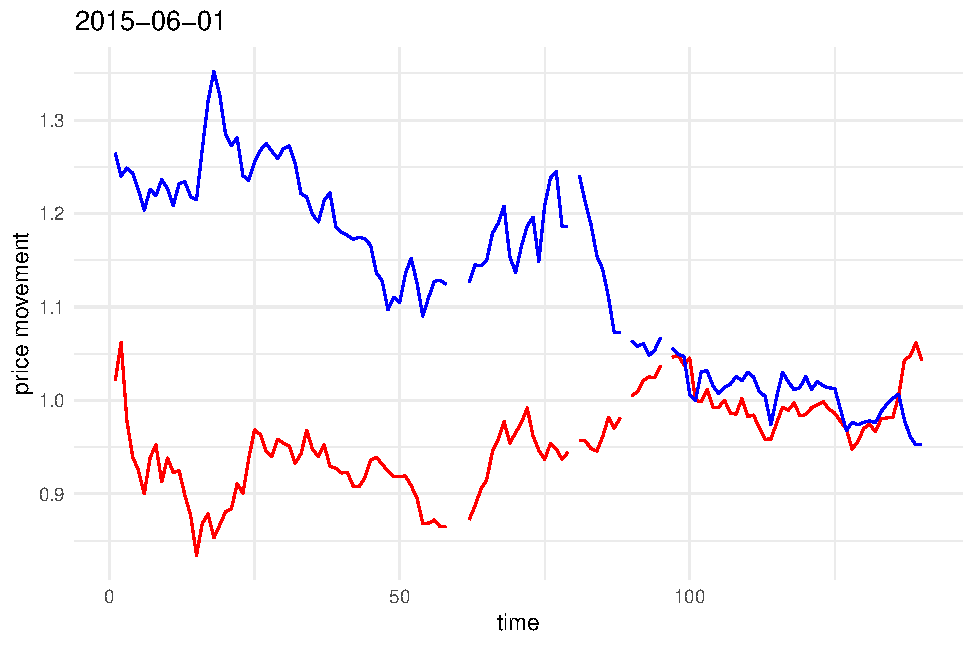
\includegraphics{plots/plot_for_2015-06-01.pdf}
    \caption{Caption}
    \label{fig:enter-label}
\end{figure}

\begin{figure}[H]
    \centering
    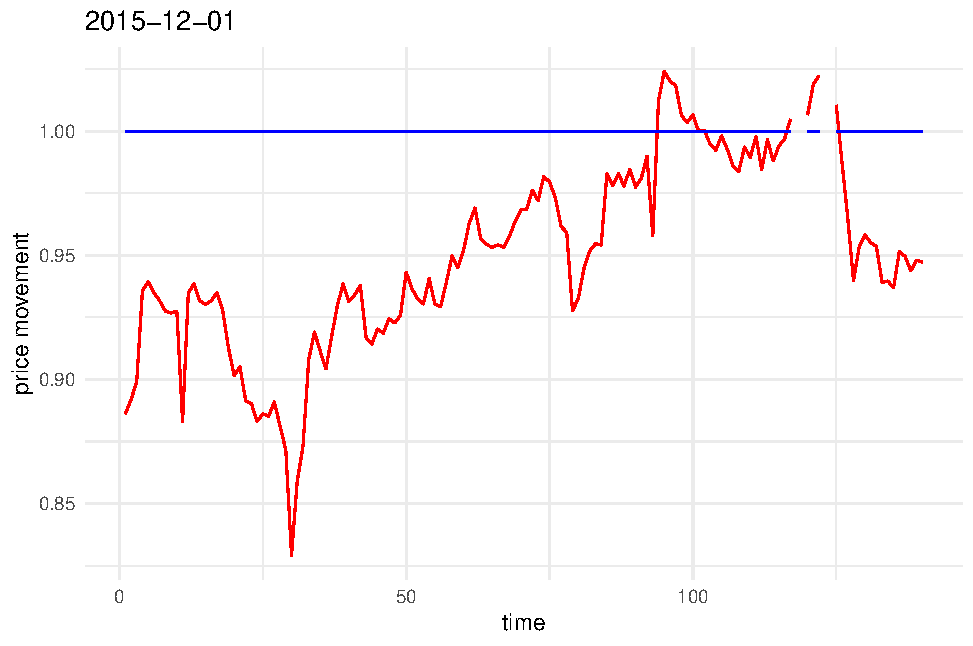
\includegraphics{plots/plot_for_2015-12-01.pdf}
    \caption{Caption}
    \label{fig:enter-label}
\end{figure}

\begin{figure}[H]
    \centering
    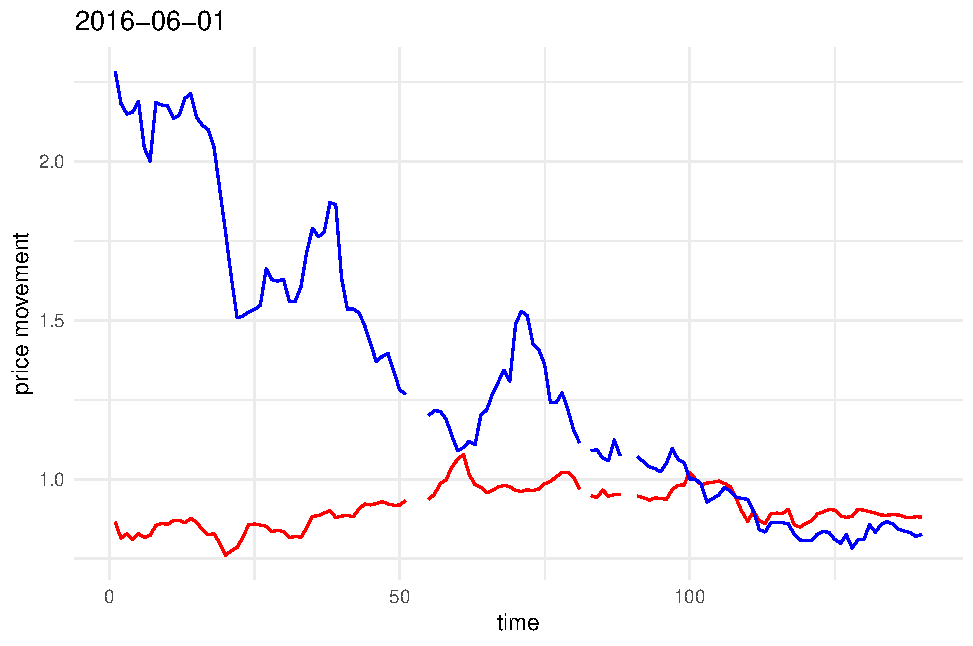
\includegraphics{plots/plot_for_2016-06-01.pdf}
    \caption{Caption}
    \label{fig:enter-label}
\end{figure}

\begin{figure}[H]
    \centering
    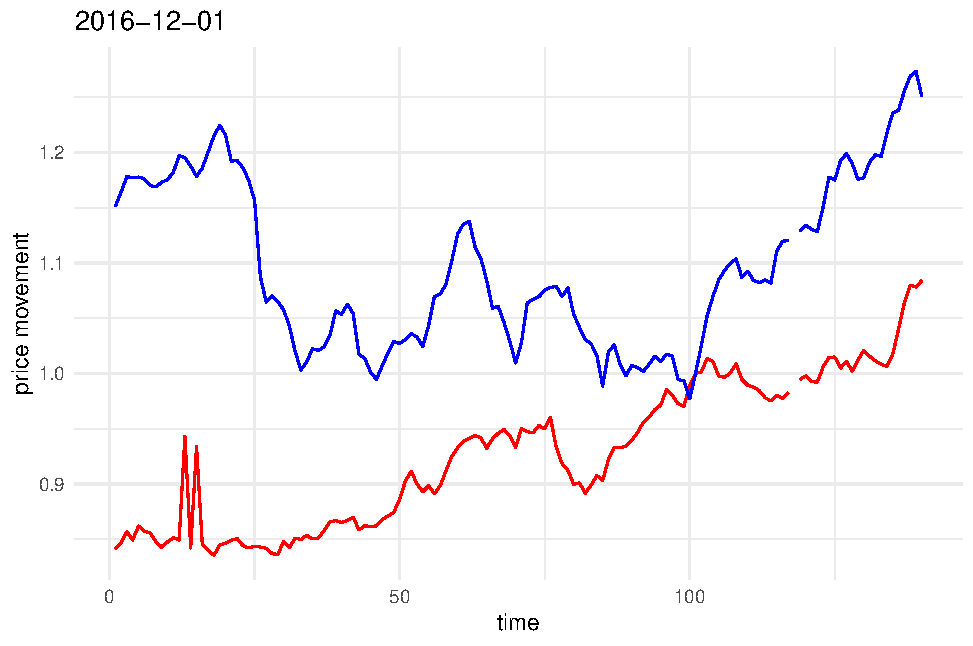
\includegraphics{plots/plot_for_2016-12-01.pdf}
    \caption{Caption}
    \label{fig:enter-label}
\end{figure}

\begin{figure}[H]
    \centering
    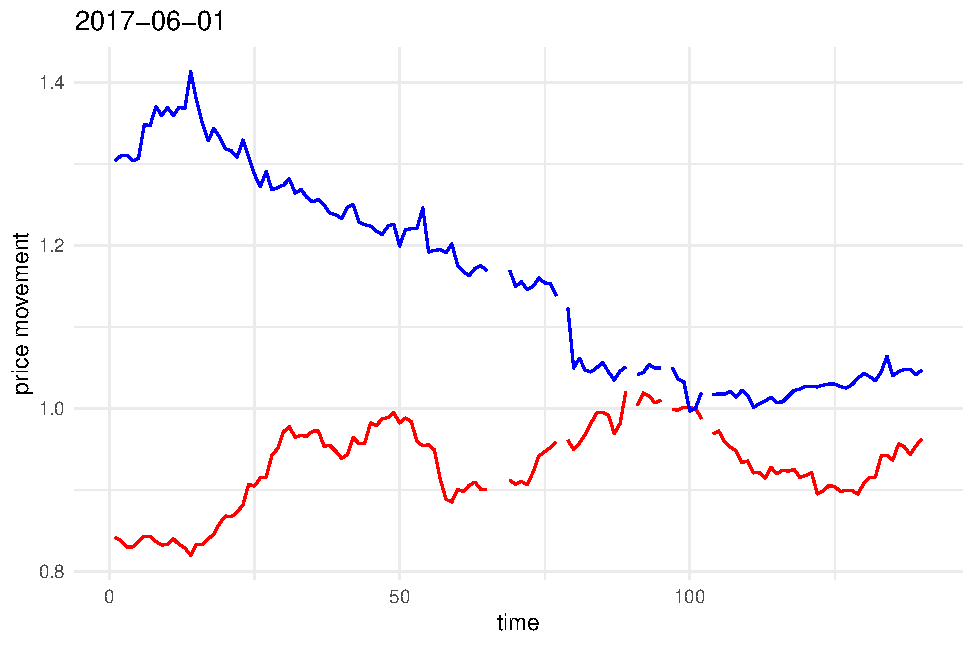
\includegraphics{plots/plot_for_2017-06-01.pdf}
    \caption{Caption}
    \label{fig:enter-label}
\end{figure}

\begin{figure}[H]
    \centering
    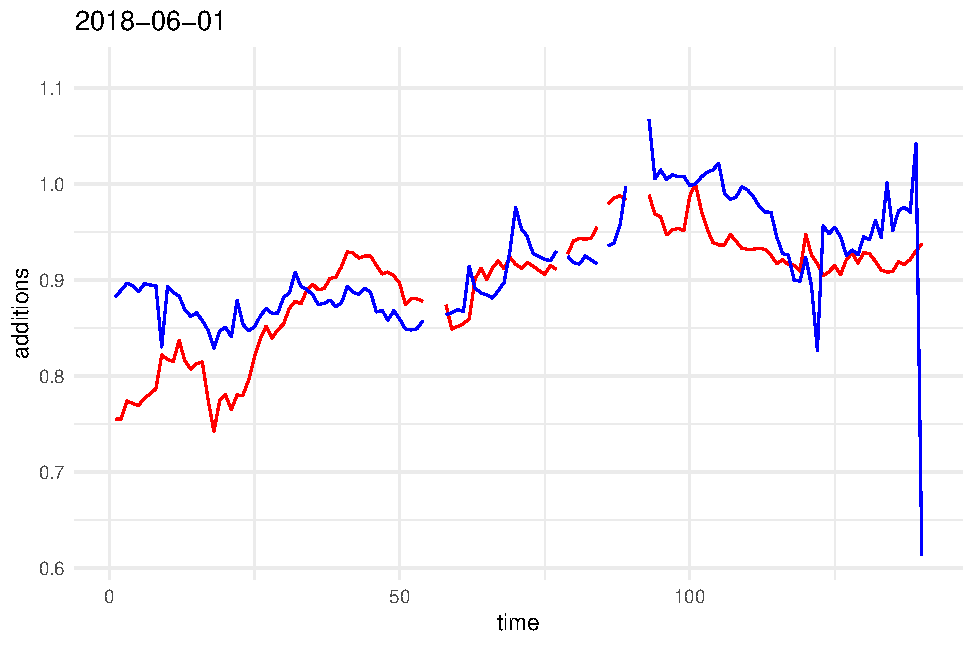
\includegraphics{plots/plot_for_2018-06-01.pdf}
    \caption{Caption}
    \label{fig:enter-label}
\end{figure}

\begin{figure}[H]
    \centering
    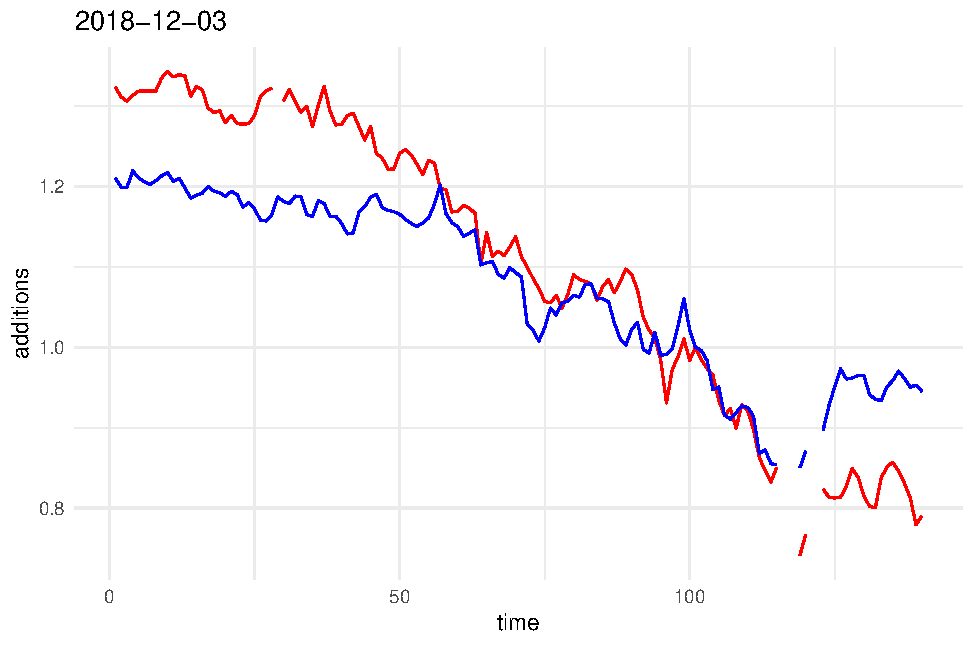
\includegraphics{plots/plot_for_2018-12-03.pdf}
    \caption{Caption}
    \label{fig:enter-label}
\end{figure}

\begin{figure}[H]
    \centering
    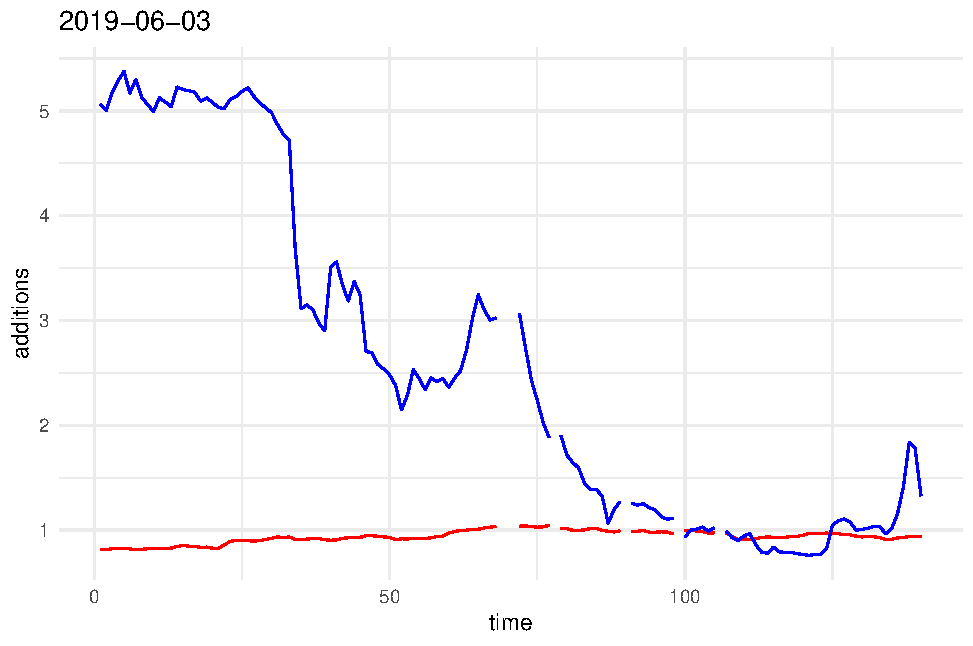
\includegraphics{plots/plot_for_2019-06-03.pdf}
    \caption{Caption}
    \label{fig:enter-label}
\end{figure}

\begin{figure}[H]
    \centering
    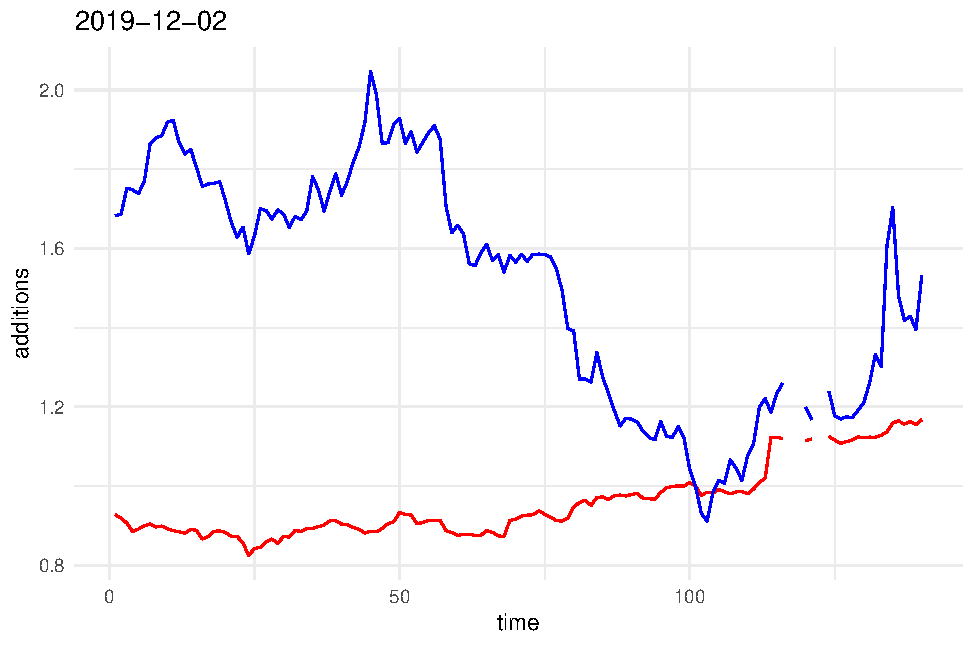
\includegraphics{plots/plot_for_2019-12-02.pdf}
    \caption{Caption}
    \label{fig:enter-label}
\end{figure}




\begin{figure}[H]
    \centering
    \caption{Decision Tree, Random Forest, and eXtreme Gradient Boosting}
    \vspace{10pt} % Adds a little space between the caption and the images
    \begin{subfigure}{0.32\linewidth}
        \centering
        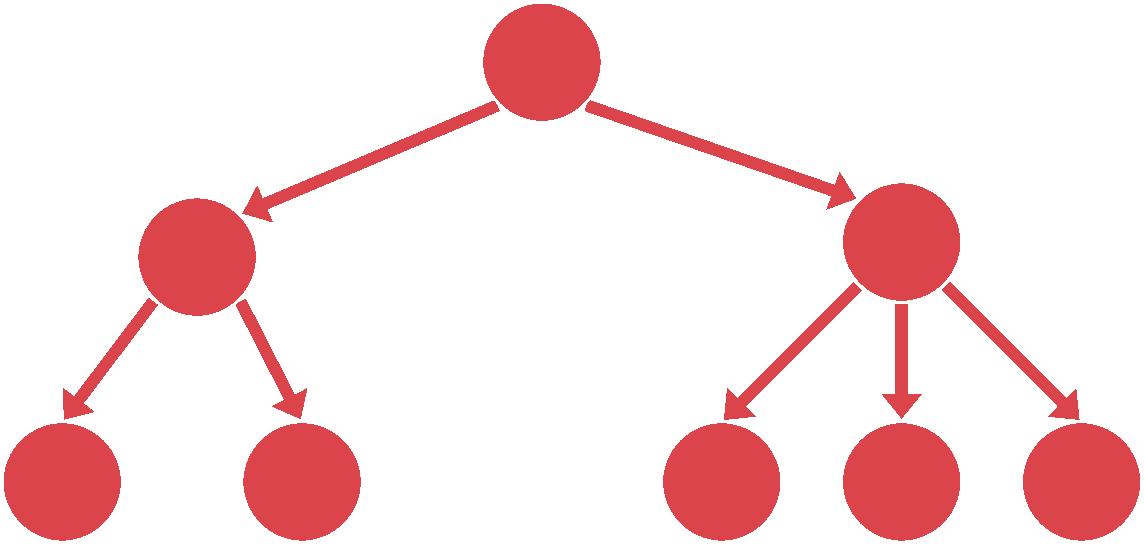
\includegraphics[width=\linewidth,keepaspectratio]{images/tree models.drawio.pdf}
        \caption{}
        \label{fig:DecisionTree}
    \end{subfigure}
    \hfill
    \begin{subfigure}{0.32\linewidth}
        \centering
        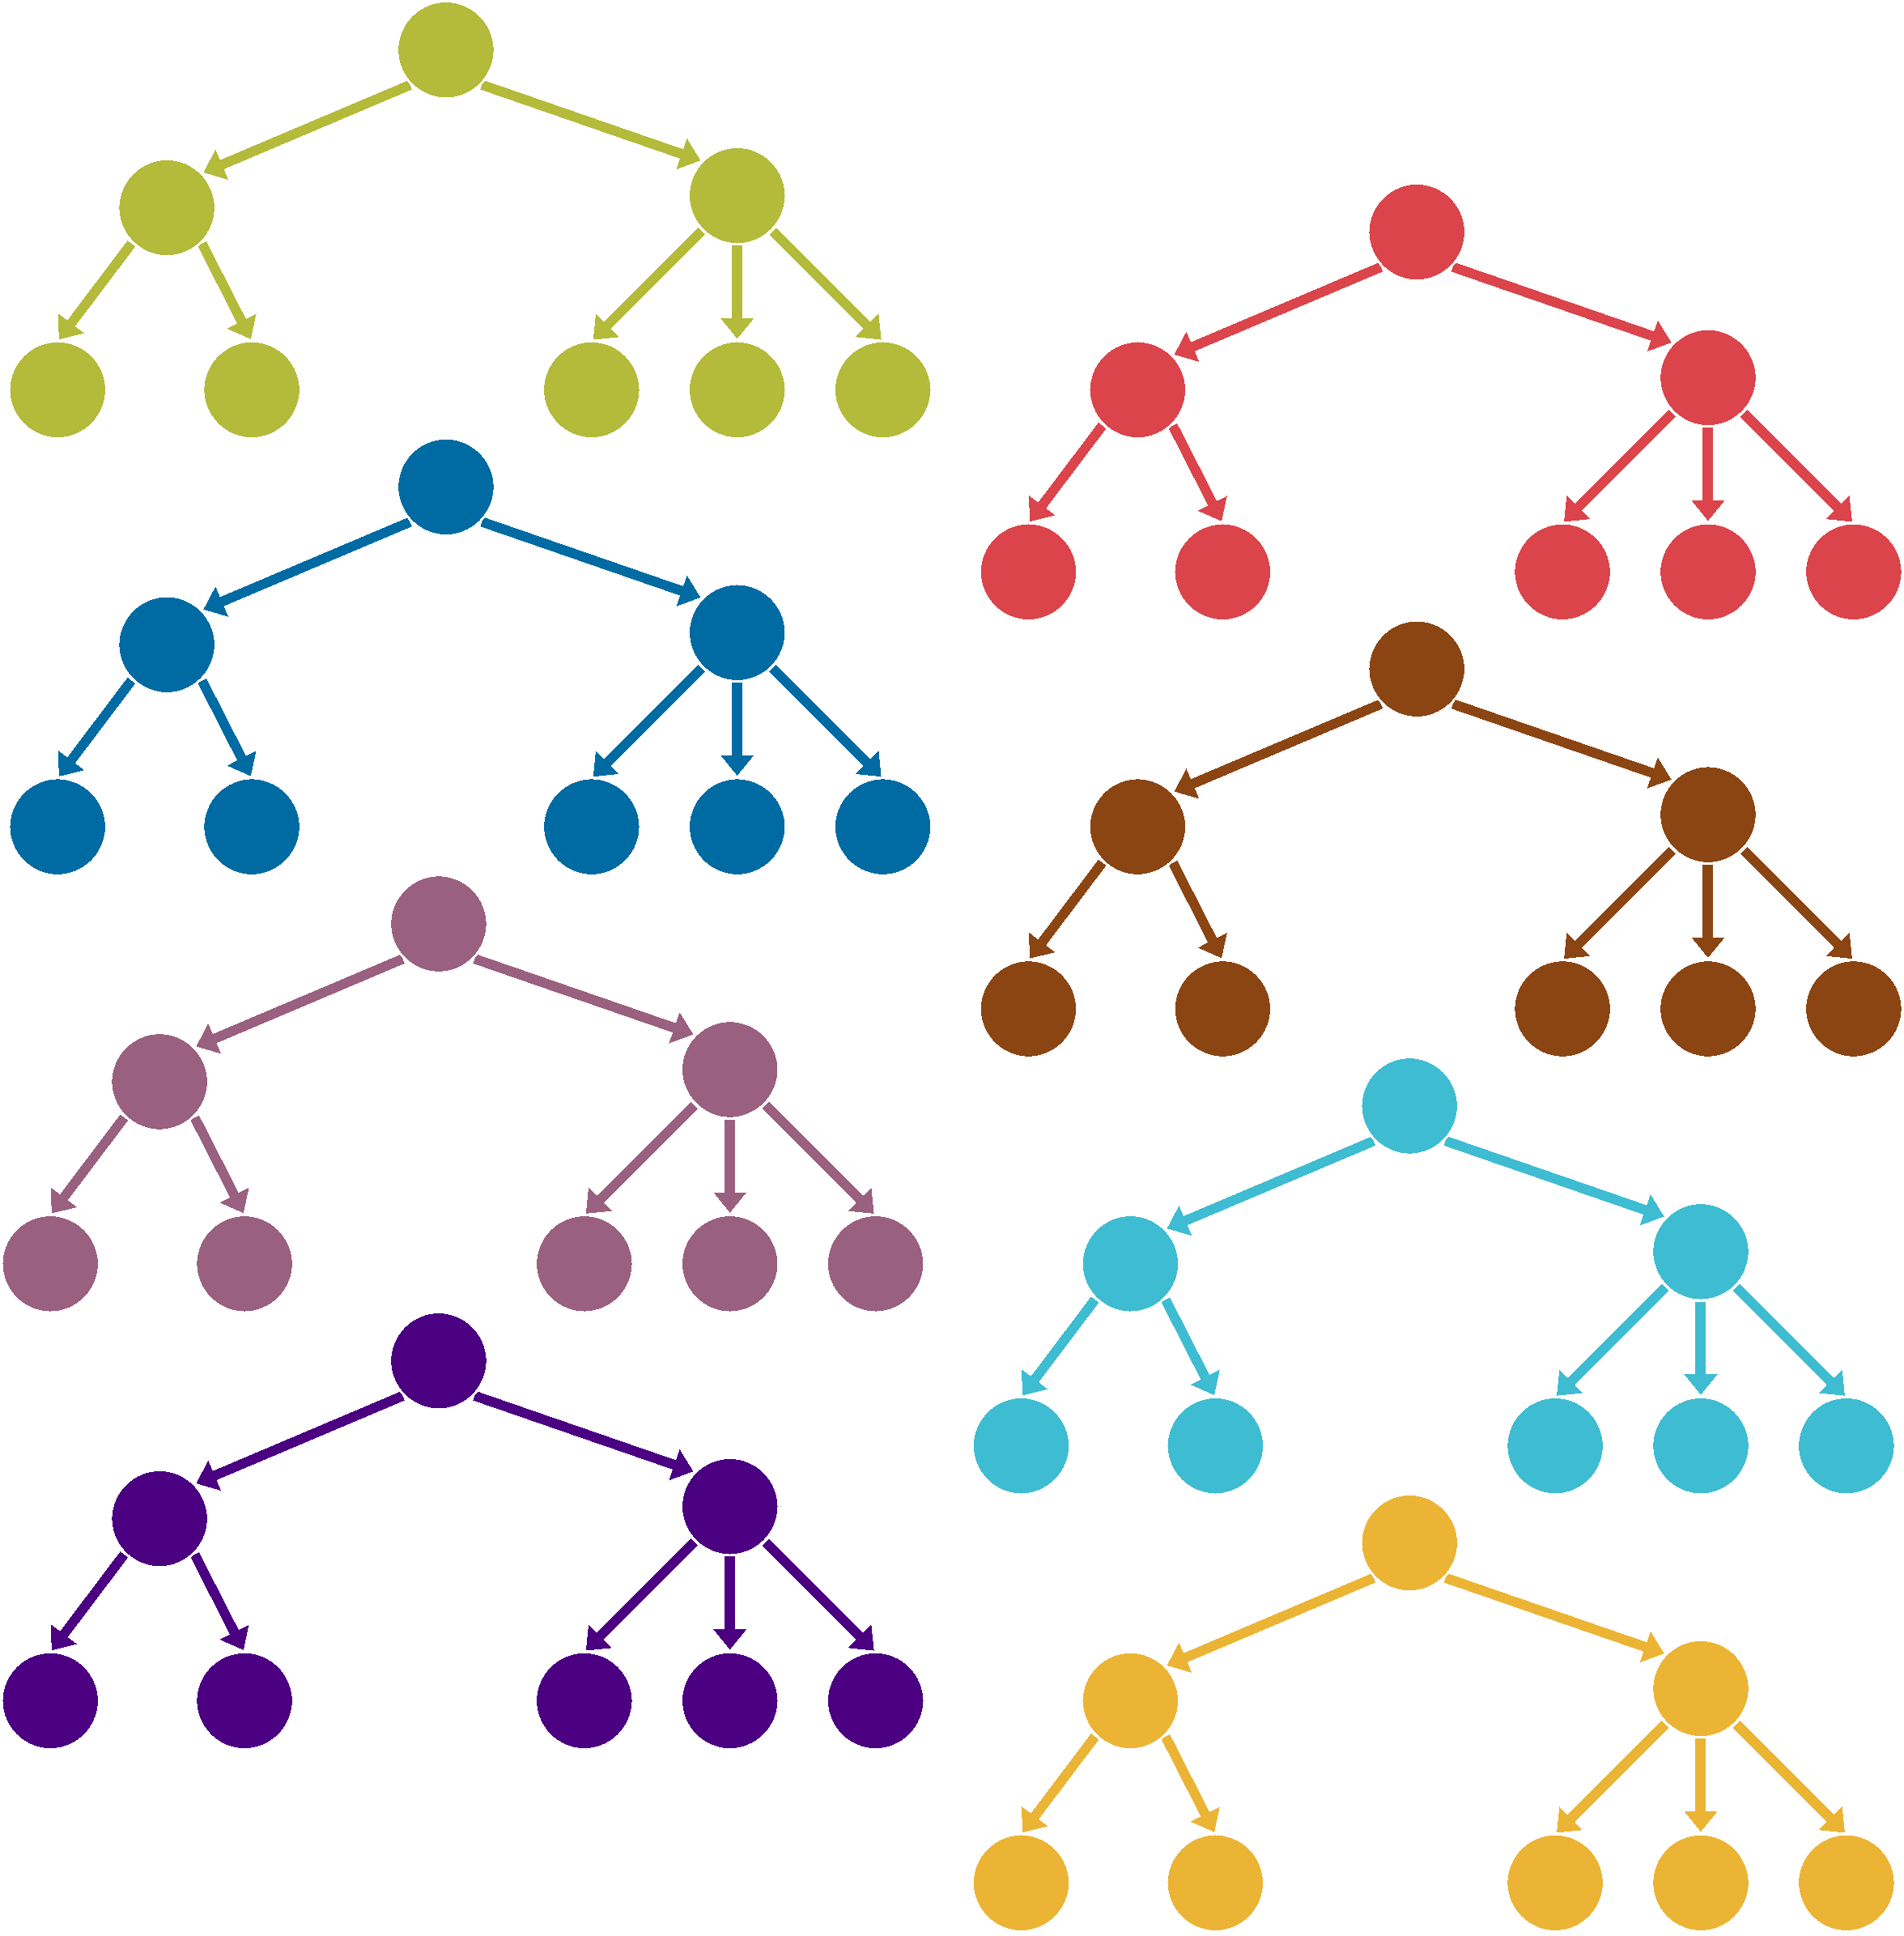
\includegraphics[width=\linewidth,keepaspectratio]{images/random forest diagram.drawio.pdf}
        \caption{}
        \label{fig:RandomForest}
    \end{subfigure}
    \hfill
    \begin{subfigure}{0.32\linewidth}
        \centering
        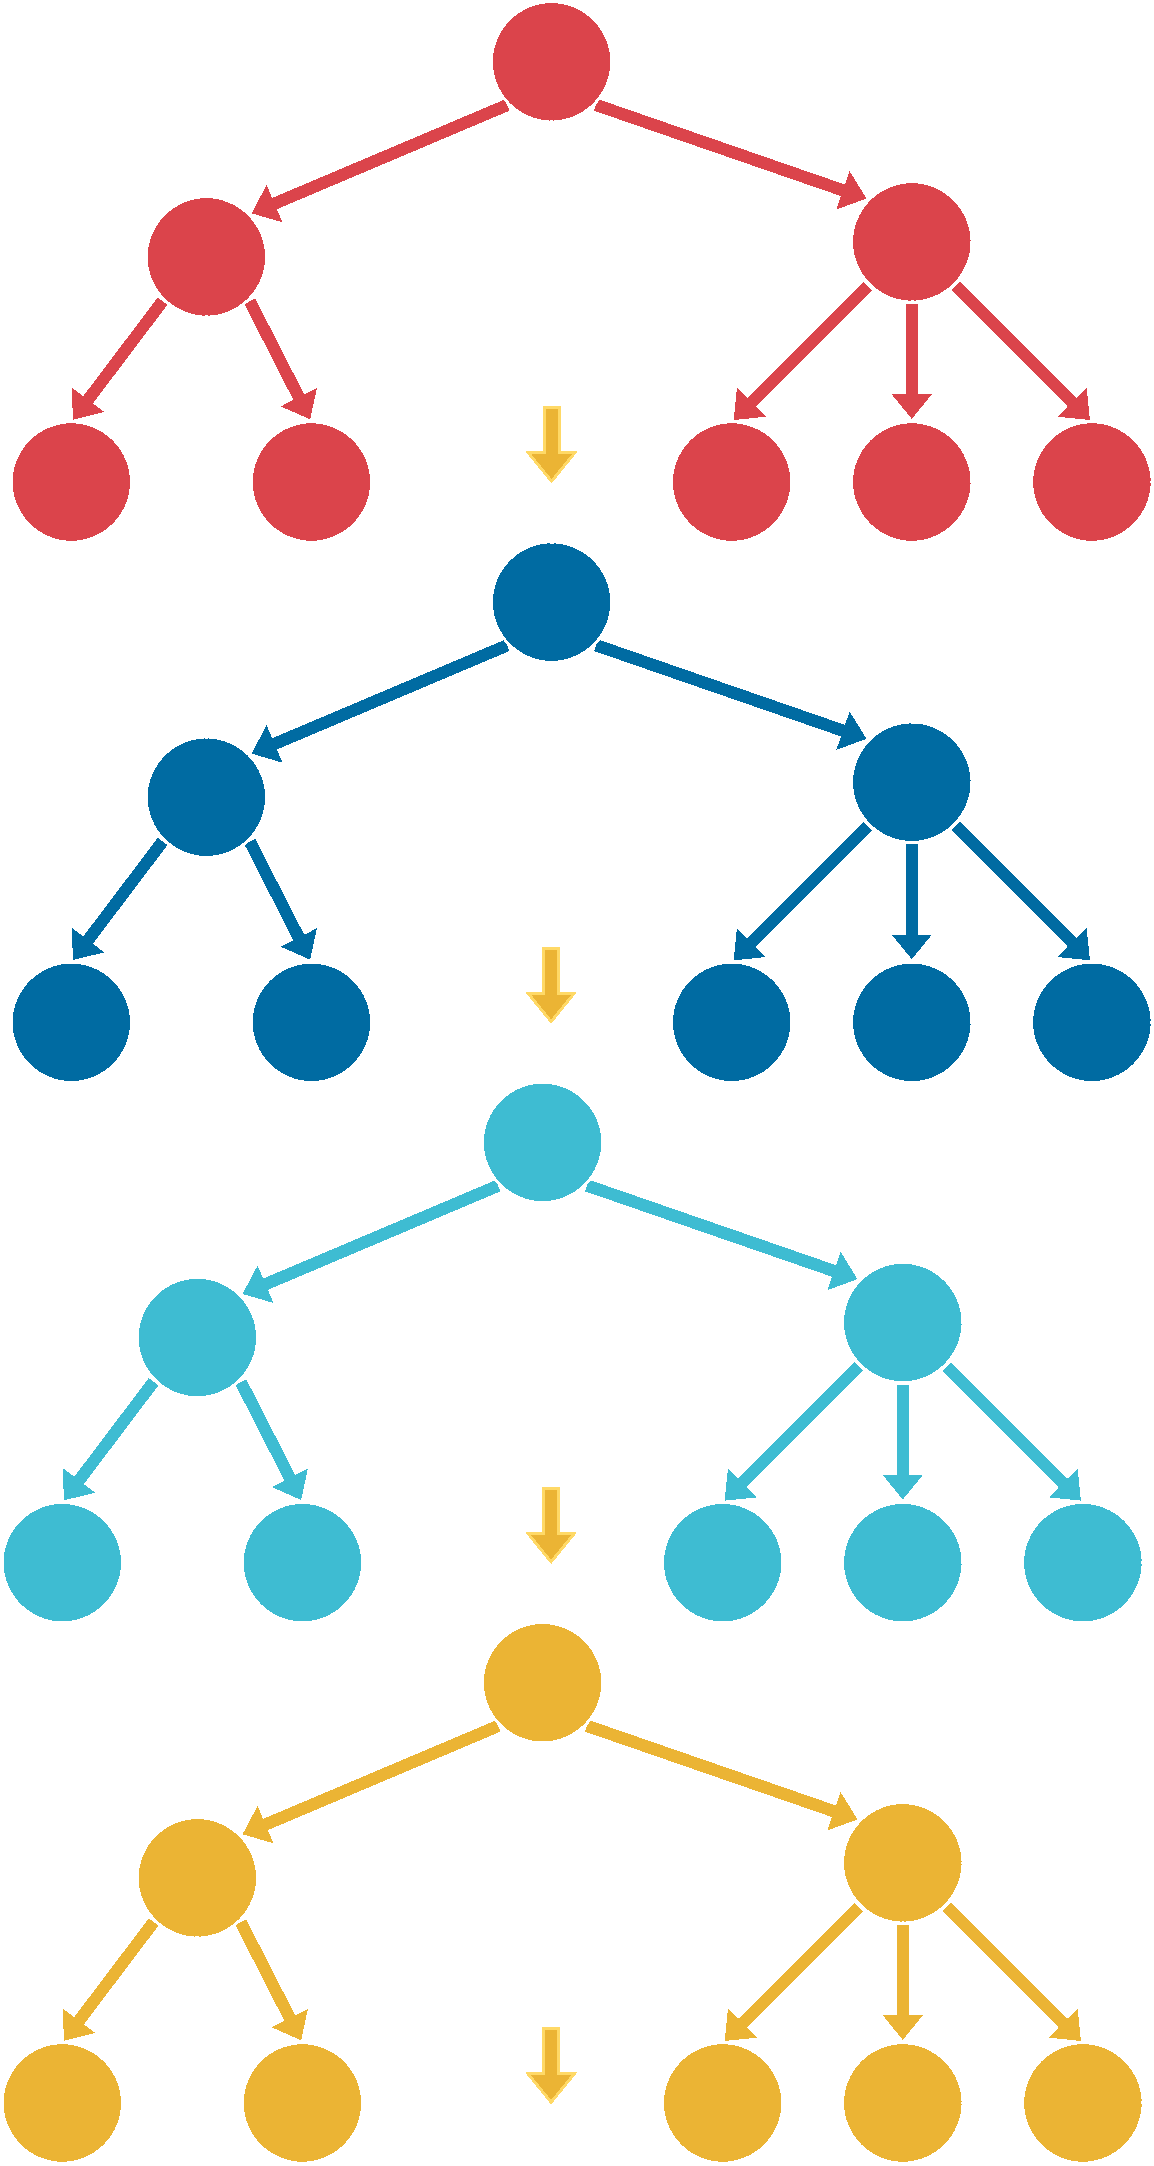
\includegraphics[width=\linewidth,keepaspectratio]{images/xgb.drawio.pdf}
        \caption{}
        \label{fig:XGBoost}
    \end{subfigure}
\end{figure}







% appendix figurer
\subsubsection{Descriptives}

\begin{figure}[H]
    \centering
    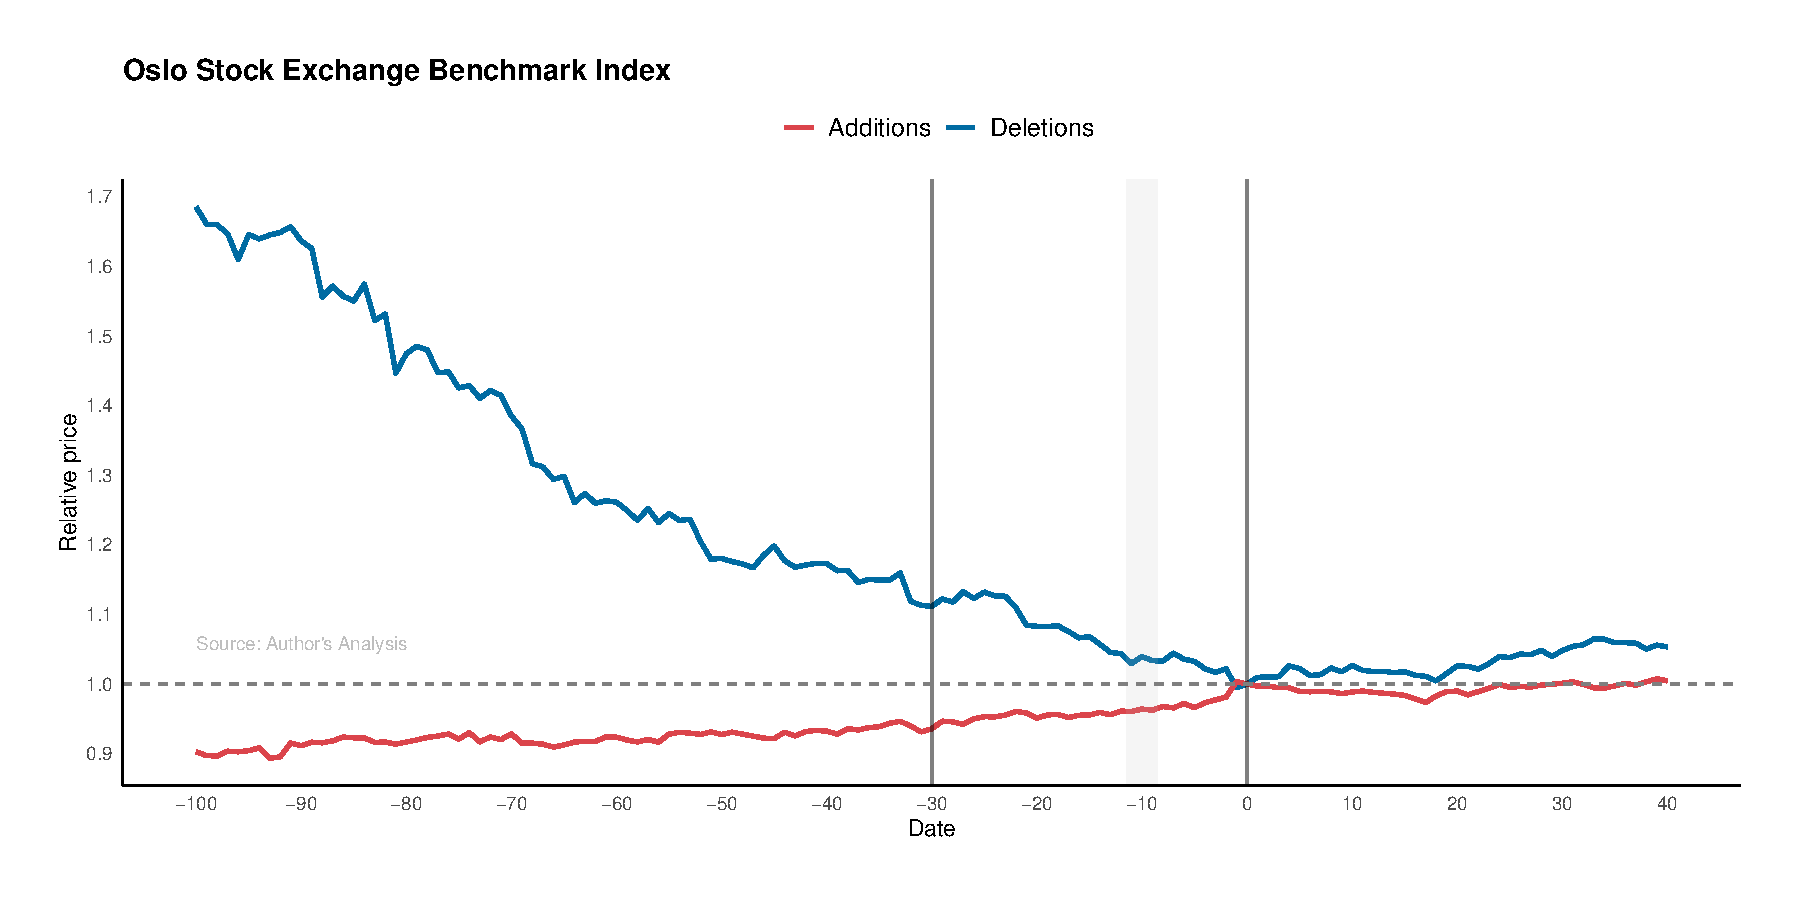
\includegraphics[width=\linewidth]{images/index_plot_126.pdf}
    \caption{Oslo Stock Exchange additions and deletions}
    \label{Oslo Stock Exchange additions and deletions}
\end{figure}

\begin{figure}[H]
    \centering
    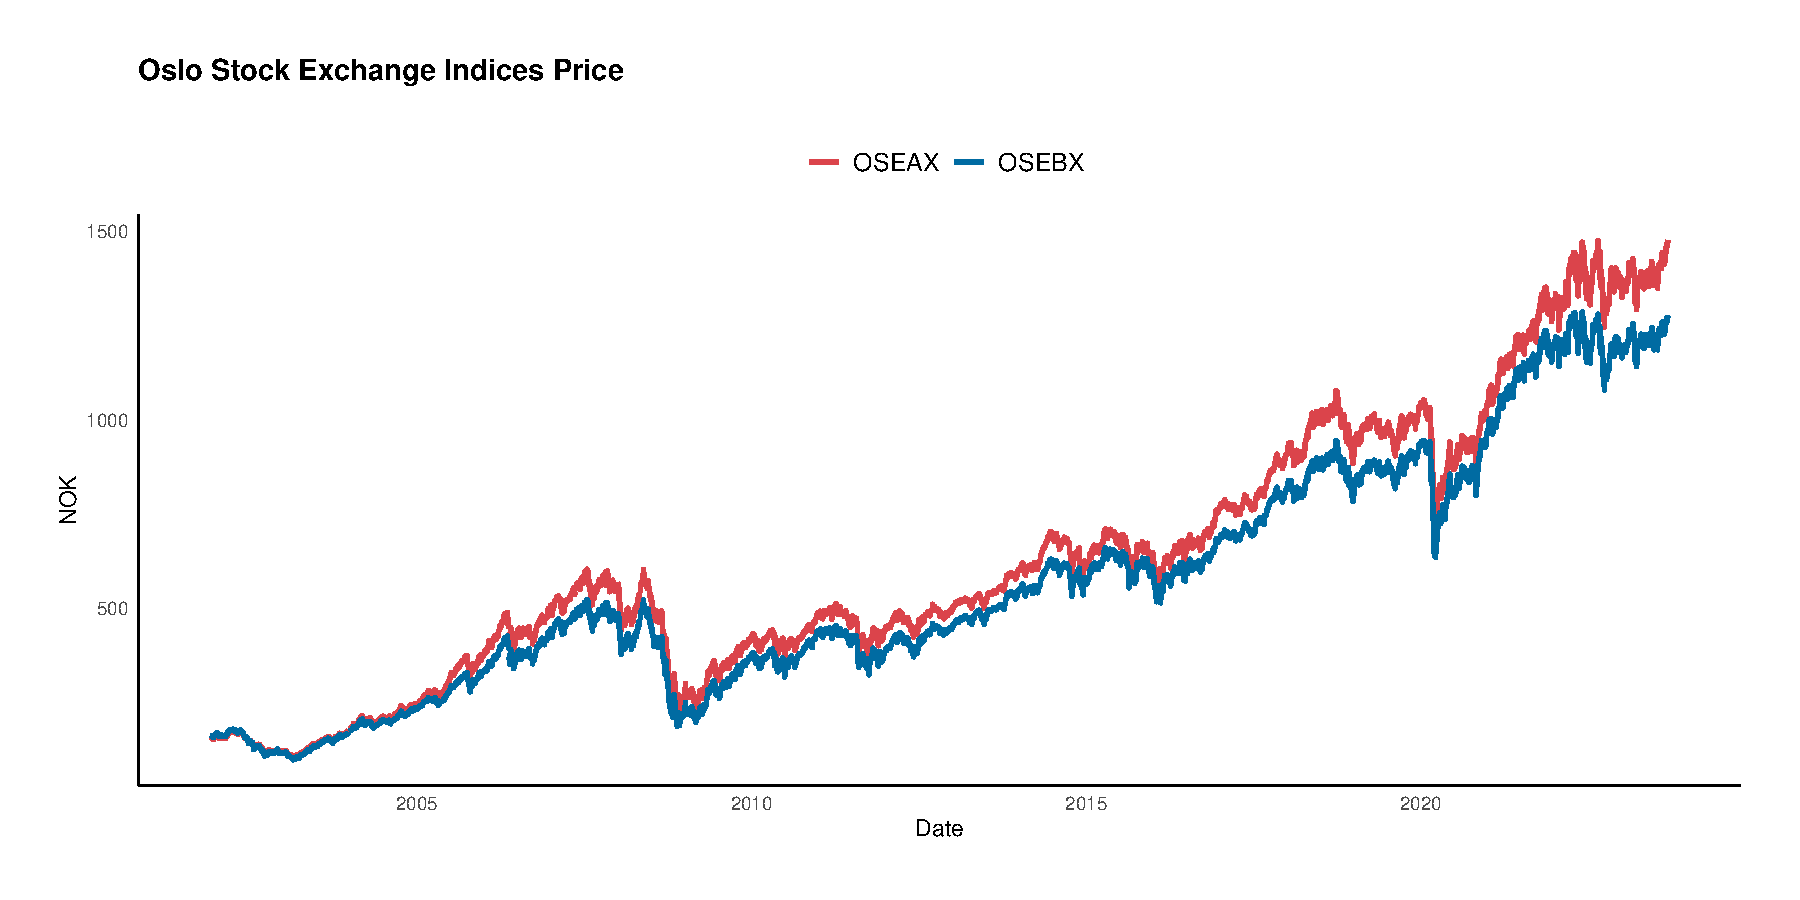
\includegraphics[width=\linewidth]{images/plot_gp_126.pdf}
    \caption{Prices over time}
    \label{Prices over time}
\end{figure}



\begin{figure}[H]
    \centering
    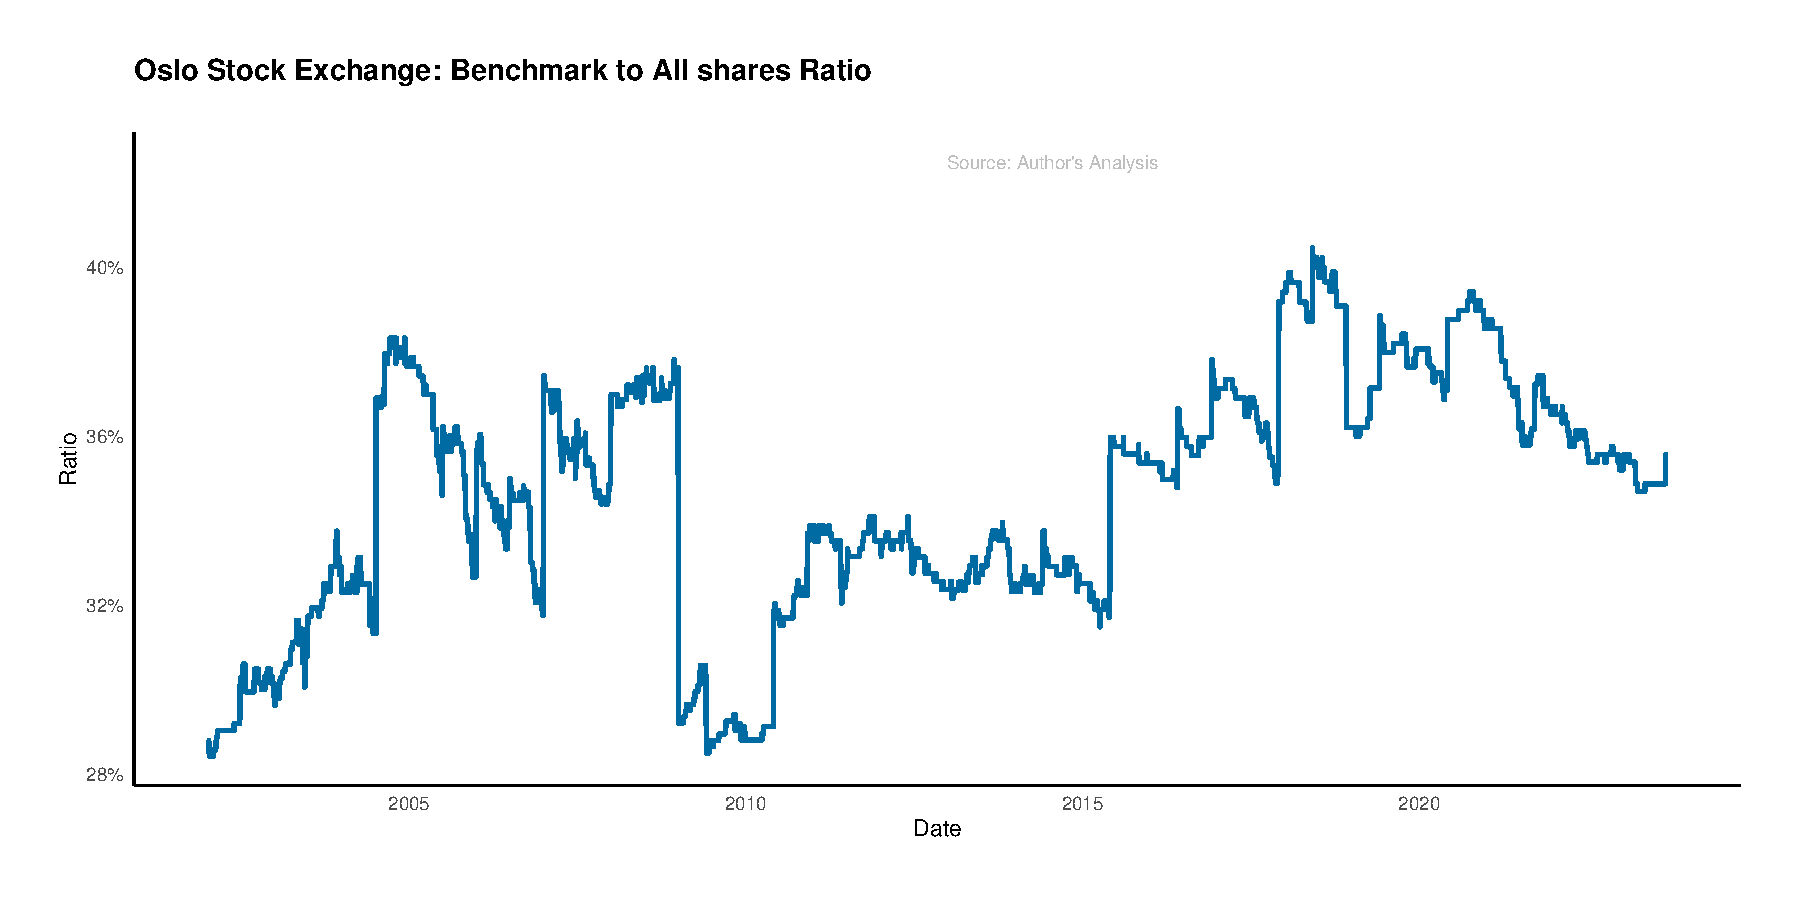
\includegraphics[width=\linewidth]{images/plot_share_126.pdf}
    \caption{Share of Benchmark to All shares over time}
    \label{Share of Benchmark to All shares over time}
\end{figure}


\begin{figure}[H]
    \centering
    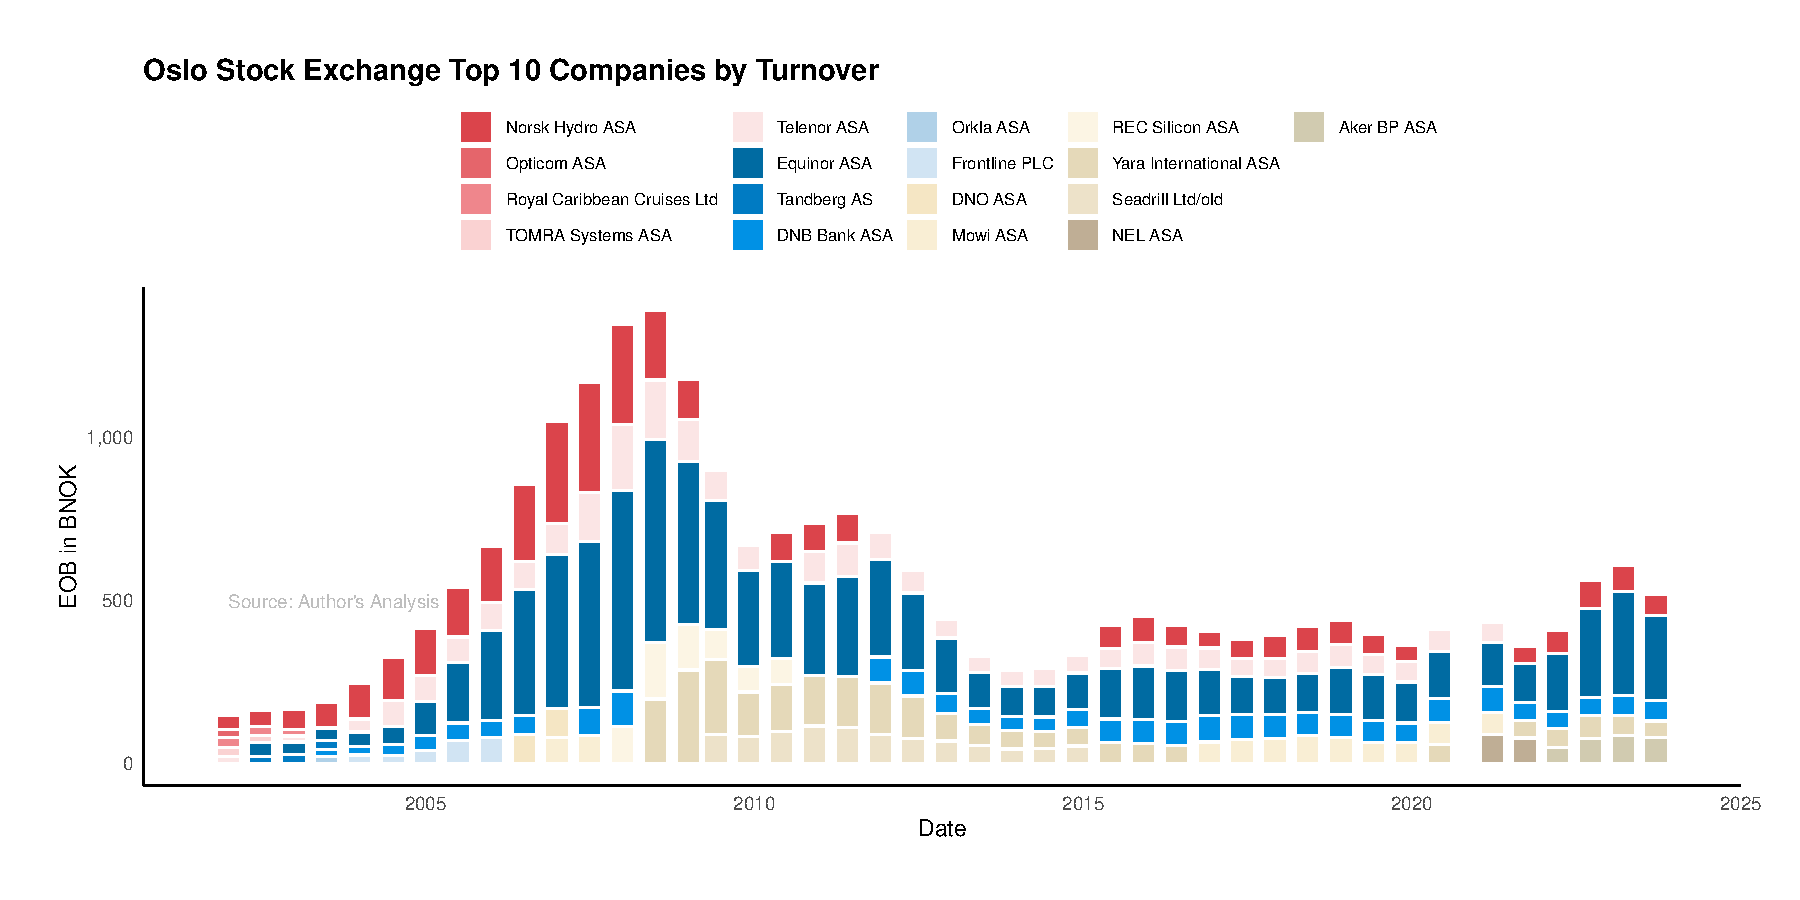
\includegraphics[width=\linewidth]{images/plot_turnover.pdf}
    \caption{Oslo Stock Exchange Benchmark Index Sector Distribution}
    \label{Oslo Stock Exchange Benchmark Index Sector Distribution}
\end{figure}

\begin{figure}[H]
    \centering
    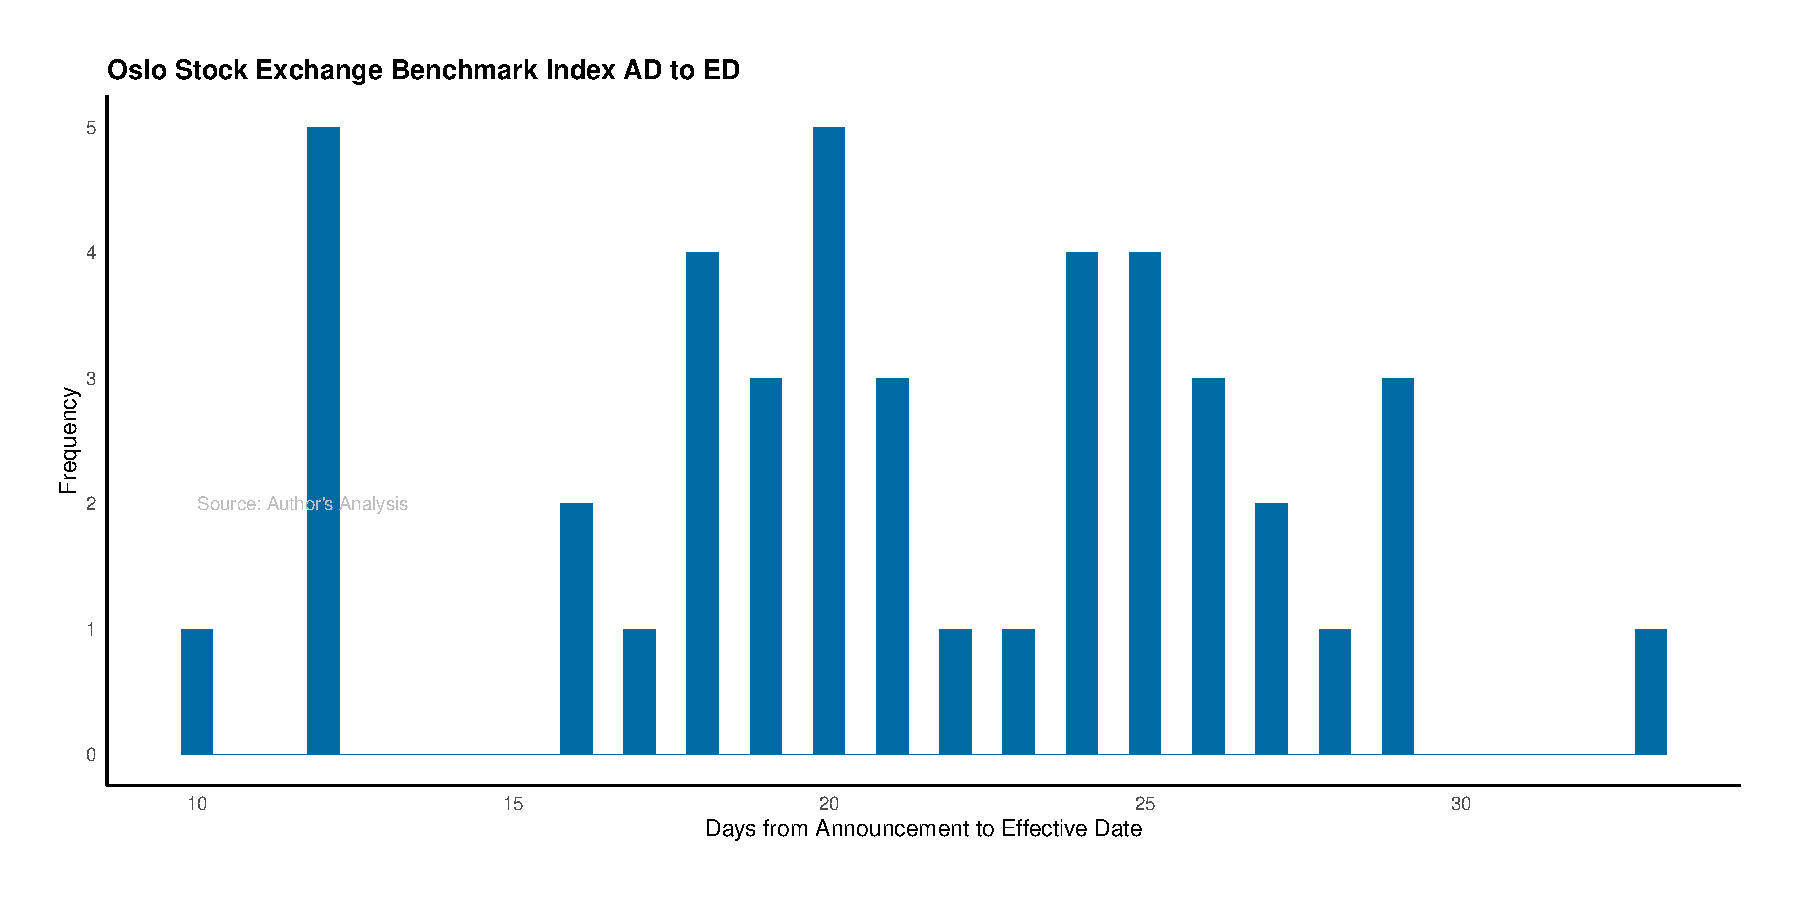
\includegraphics[width=\linewidth]{images/plot_ad_to_ed.pdf}
    \caption{Oslo Stock Exchange Benchmark Index Sector Distribution}
    \label{Oslo Stock Exchange Benchmark Index Sector Distribution}
\end{figure}

\begin{figure}[H]
    \centering
    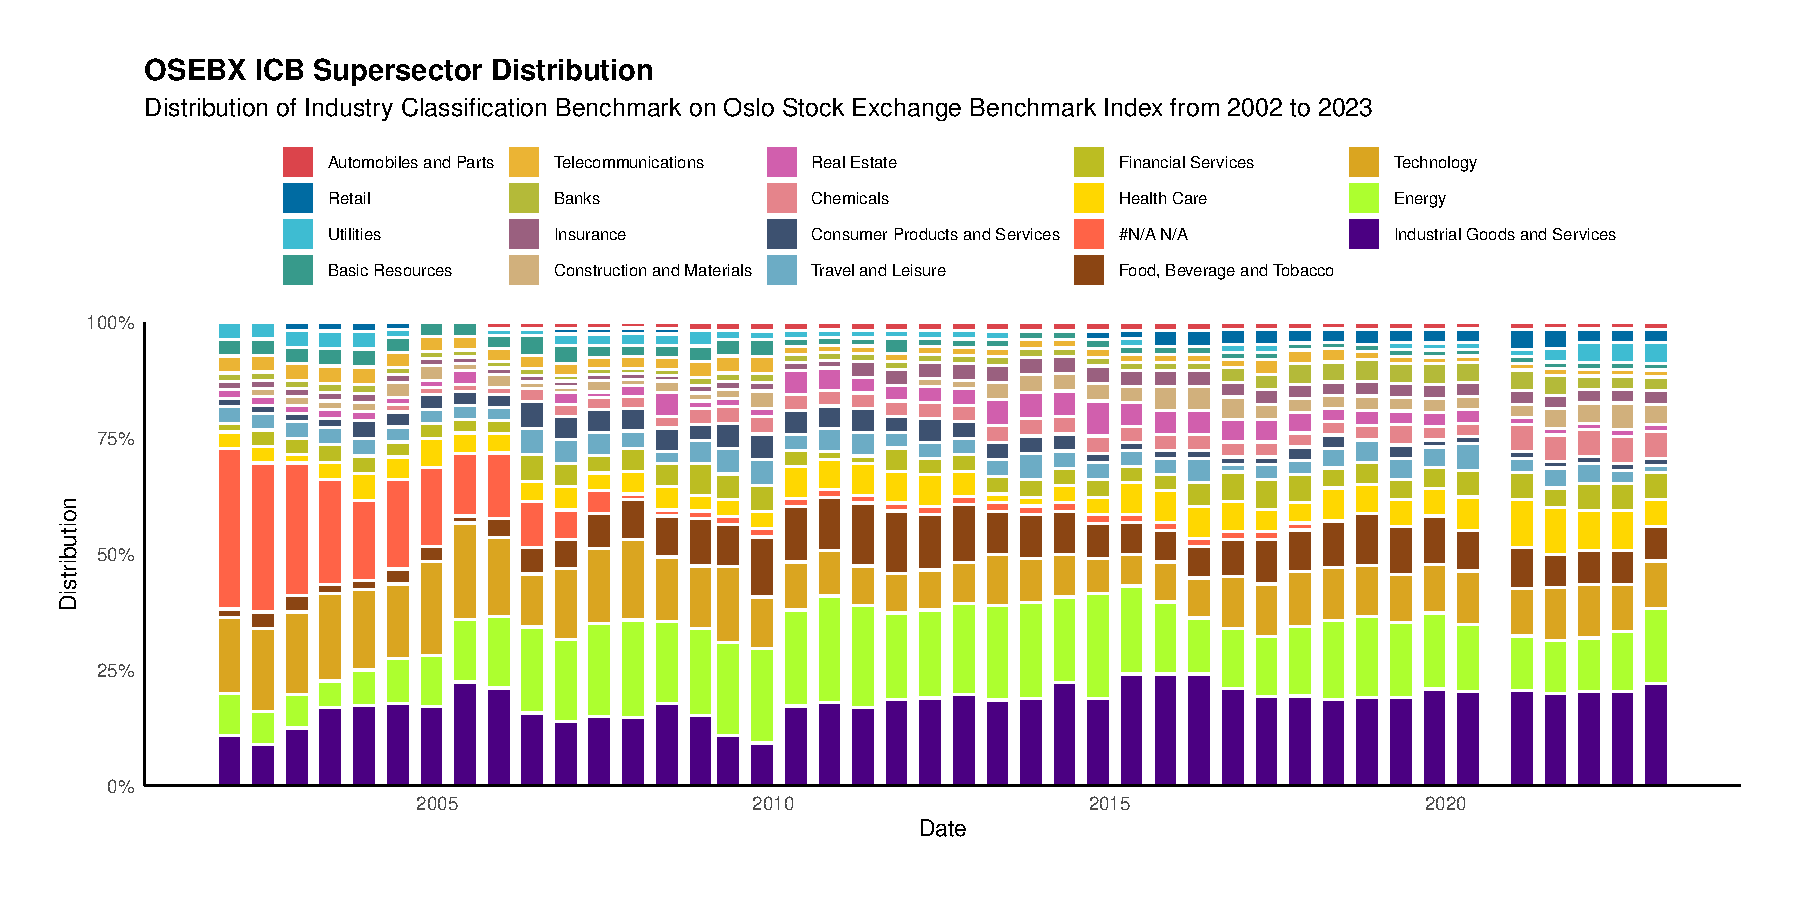
\includegraphics[width=\linewidth]{images/plot_sectors.pdf}
    \caption{Oslo Stock Exchange Benchmark Index Sector Distribution}
    \label{Oslo Stock Exchange Benchmark Index Sector Distribution}
\end{figure}

\begin{figure}[H]
    \centering
    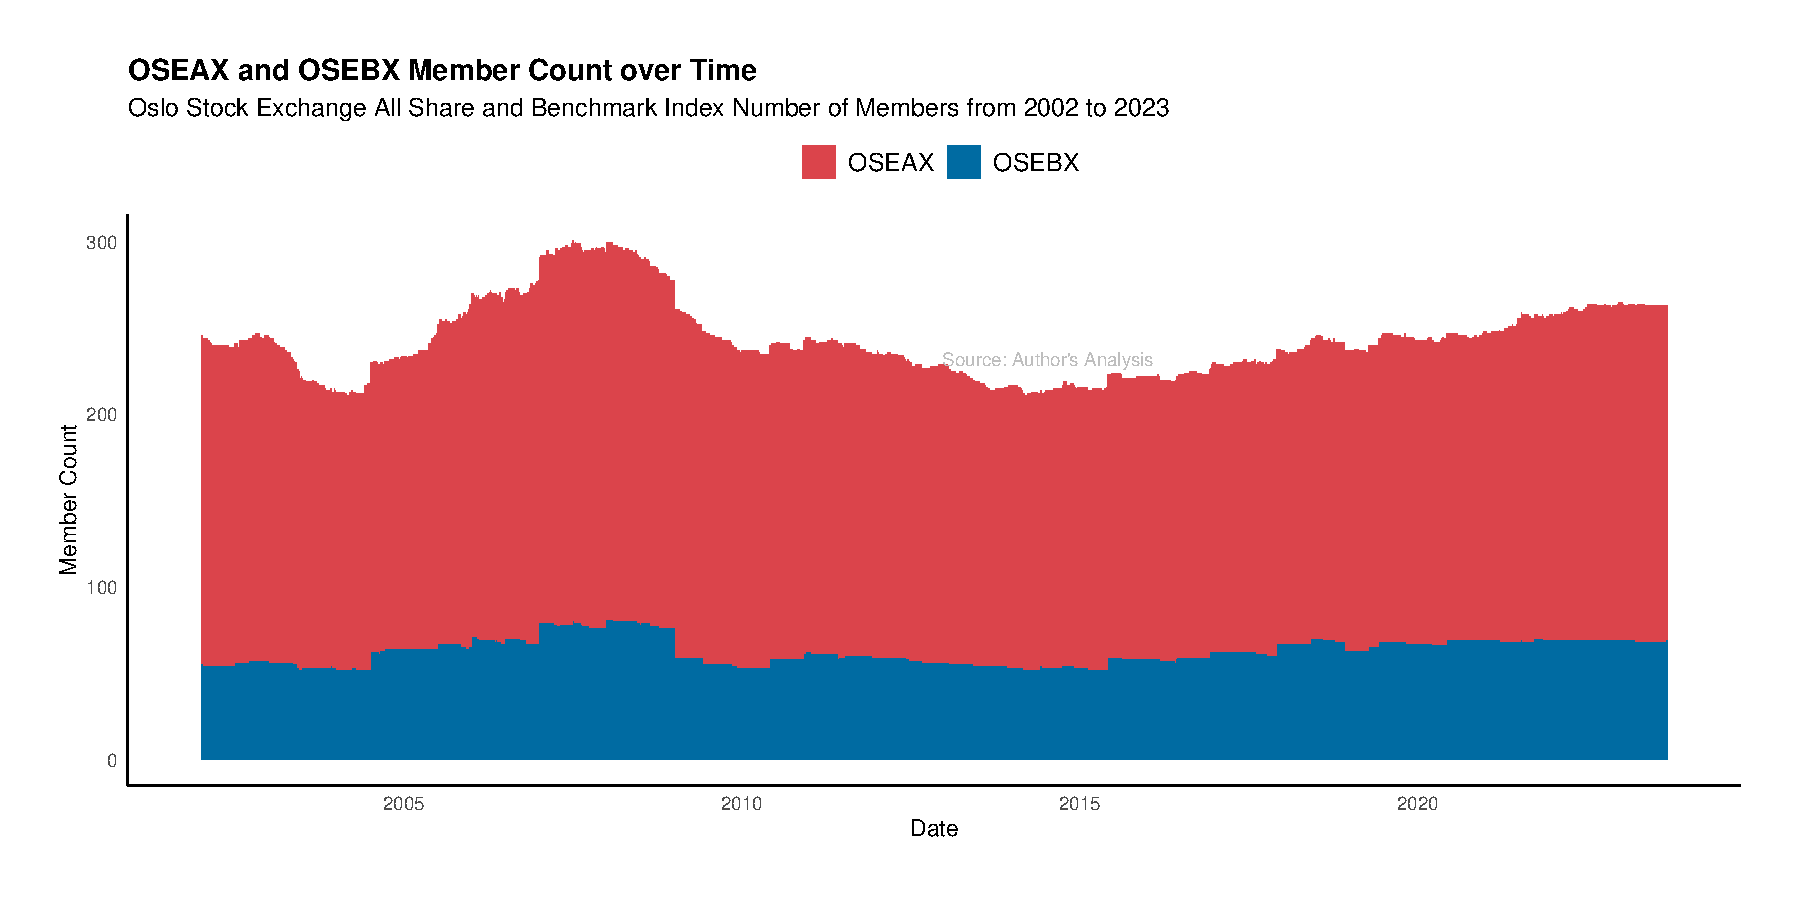
\includegraphics[width=\linewidth]{images/plot_memb_126.pdf}
    \caption{Members over time}
    \label{Members over time}
\end{figure}









% TABLES OF CONSTITUENTS AND CHANGES


\newpage
\clearpage
\subsection{Overview of additions and deletions to OSEBX}

\begin{table}[H]
\centering
\begin{tabularx}{\textwidth}{XXX}
\toprule
Company & Additions & Deletions \\ 
\midrule
ABG Sundal Collier Holding ASA & 2020-05-29, 2006-06-30 & 2016-11-30 \\ 
AF Gruppen ASA & 2013-05-31 &  \\ 
AMSC ASA & 2019-05-31, 2016-11-30, 2014-05-30 & 2021-03-19, 2017-05-31, 2016-05-31 \\ 
Akastor ASA & 2006-06-30 & 2015-05-29 \\ 
Aker ASA & 2011-11-30, 2009-11-30, 2006-06-30 & 2010-05-31, 2009-05-29 \\ 
Aker BP ASA & 2012-05-31 &  \\ 
Aker BioMarine ASA & 2011-05-31, 2007-06-29 & 2011-11-30, 2007-12-30 \\ 
Aker Carbon Capture ASA & 2023-03-17, 2022-03-18 & 2022-09-16 \\ 
Aker Horizons ASA & 2021-09-17 &  \\ 
Aker Solutions ASA & 2016-11-30 & 2016-05-31 \\ 
Algeta ASA & 2009-11-30 &  \\ 
Altinex AS & 2006-12-29 &  \\ 
Andvord Tybring-Gjedde & 2006-06-30 &  \\ 
Archer Ltd & 2011-05-31 & 2011-11-30 \\ 
ArcticZymes Technologies ASA & 2021-03-19, 2014-05-30 & 2017-05-31 \\ 
Arendals Fossekompani ASA & 2022-03-18 &  \\ 
Arribatec Group ASA & 2006-06-30 & 2011-11-30 \\ 
Asetek A/S & 2016-11-30 & 2021-03-19, 2014-11-28 \\ 
Atea ASA & 2006-06-30 &  \\ 
Austevoll Seafood ASA & 2018-05-31, 2007-06-29 & 2020-05-29, 2013-11-29 \\ 
AutoStore Holdings Ltd & 2022-03-18 &  \\ 
Avance Gas Holding Ltd & 2020-05-29, 2015-05-29 & 2022-03-18, 2016-11-30 \\ 
Axactor ASA & 2016-05-31, 2006-06-30 & 2021-09-17, 2007-06-29 \\ 
Axel Springer Norway AS & 2006-12-29 &  \\ 
BW Gas AS & 2006-06-30 & 2007-06-29 \\ 
BW LPG Ltd & 2017-11-30, 2014-05-30 & 2016-11-30 \\ 
BW Offshore Ltd & 2018-05-31, 2010-11-30, 2007-06-29 & 2021-03-19, 2011-05-31, 2008-06-30 \\ 
BWG Homes ASA & 2009-05-29, 2006-06-30 & 2008-12-30 \\ 
Bakkafrost P/F & 2014-05-30, 2011-11-30 & 2013-05-31, 2010-11-30 \\ 
Bank Norwegian ASA & 2017-11-30, 2016-11-30 & 2017-05-31 \\ 
Bergenbio ASA & 2018-05-31 & 2023-03-17 \\ 
Bonheur ASA & 2019-11-29 &  \\ 
Borr Drilling Ltd & 2023-03-17, 2017-11-30 & 2020-05-29 \\ 
Borregaard ASA & 2021-03-19 &  \\ 
Bouvet ASA & 2020-05-29 &  \\ 
COSL Holding AS & 2006-12-29 &  \\ 
Cadeler A/S & 2022-09-16 &  \\ 
Carasent ASA & 2021-03-19, 2006-06-30 & 2023-03-17, 2007-12-30 \\ 
Cermaq Group AS & 2006-06-30 & 2014-05-30 \\ 
Circio Holding ASA & 2017-11-30 & 2018-11-30 \\ 
\bottomrule
\end{tabularx}
\end{table}
\newpage
\clearpage

\begin{table}[H]
\centering
\begin{tabularx}{\textwidth}{XXX}
\toprule
Company & Additions & Deletions \\ 
\midrule
Cloudberry Clean Energy ASA & 2022-03-18 &  \\ 
Copeinca ASA & 2009-11-30, 2007-12-30 & 2010-05-31, 2008-12-30 \\ 
Crayon Group Holding ASA & 2020-05-29 &  \\ 
Crew Gold Corp & 2006-06-30 & 2007-06-29 \\ 
DNB Bank ASA & 2006-06-30 &  \\ 
DNO ASA & 2006-06-30 &  \\ 
Data Respons ASA & 2019-11-29, 2006-12-29 & 2009-11-30 \\ 
Dolphin Drilling ASA & 2006-06-30 & 2015-11-30 \\ 
Ekornes ASA & 2006-06-30 &  \\ 
Electromagnetic Geoservices ASA & 2012-11-30 & 2013-11-29 \\ 
Elkem ASA & 2019-05-31 &  \\ 
Elmera Group ASA & 2019-05-31 &  \\ 
Eltek AS & 2010-05-31, 2006-06-30 & 2008-12-30 \\ 
Ensurge Micropower ASA & 2015-05-29 & 2019-05-31 \\ 
Equinor ASA & 2006-06-30 &  \\ 
Europris ASA & 2015-11-30 &  \\ 
Evry AS & 2017-11-30 &  \\ 
Expert AS & 2006-06-30 &  \\ 
FLEX LNG Ltd & 2021-09-17 &  \\ 
Fjord1 AS & 2018-05-31 & 2021-03-19 \\ 
Frontline PLC & 2015-05-29, 2006-06-30 & 2013-05-31 \\ 
Funcom Se & 2017-11-30, 2012-05-31, 2006-06-30 & 2018-11-30, 2012-11-30, 2008-12-30 \\ 
Gaming Innovation Group Inc & 2021-09-17, 2017-05-31, 2016-05-31 & 2022-09-16, 2021-03-19, 2016-11-30 \\ 
Gjensidige Forsikring ASA & 2011-05-31 &  \\ 
Golden Ocean Group Ltd/Old & 2006-12-29 &  \\ 
Grieg Seafood ASA & 2017-05-31 & 2021-09-17 \\ 
Hafnia Ltd & 2022-09-16 &  \\ 
Hafslund ASA & 2016-11-30, 2006-12-29, 2006-06-30 & 2013-11-29, 2009-05-29 \\ 
Hexagon Composites ASA & 2019-05-31, 2016-05-31, 2014-05-30 & 2018-11-30, 2014-11-28 \\ 
IDEX Biometrics ASA & 2015-05-29 & 2021-09-17 \\ 
IMAREX ASA & 2007-12-30 & 2009-11-30 \\ 
Itera ASA & 2007-06-29 & 2008-06-30 \\ 
Jason Shipping AS & 2007-12-30, 2006-06-30 & 2009-05-29, 2007-06-29 \\ 
Jinhui Shipping \& Transportation Ltd & 2010-11-30, 2007-06-29 & 2011-05-31, 2008-12-30 \\ 
Kahoot! ASA & 2021-09-17 &  \\ 
Karo Pharma Norge AS & 2014-11-28, 2010-05-31 & 2013-05-31 \\ 
Kid ASA & 2021-03-19 &  \\ 
Kitron ASA & 2016-11-30 &  \\ 
Komplett ASA & 2006-12-29 & 2008-12-30 \\ 
Kongsberg Automotive ASA & 2006-06-30 &  \\ 
\bottomrule
\end{tabularx}
\end{table}
\newpage
\clearpage

\begin{table}[H]
\centering
\begin{tabularx}{\textwidth}{XXX}
\toprule
Company & Additions & Deletions \\ 
\midrule
Kongsberg Gruppen ASA & 2010-05-31, 2008-06-30 & 2009-11-30 \\ 
Leroy Seafood Group ASA & 2016-11-30, 2009-11-30, 2006-06-30 & 2014-11-28, 2009-05-29 \\ 
Link Mobility Group ASA & 2017-05-31 &  \\ 
MPC Container Ships ASA & 2018-11-30 &  \\ 
Magnora ASA & 2006-06-30 & 2012-05-31 \\ 
Mamut AS & 2007-06-29 & 2010-05-31 \\ 
Medistim ASA & 2020-05-29 & 2021-09-17 \\ 
Microsoft Development Center Norway AS & 2006-06-30 &  \\ 
Morpol ASA & 2010-11-30 & 2012-05-31 \\ 
Mowi ASA & 2006-06-30 &  \\ 
Multiconsult ASA & 2021-09-17, 2015-11-30 & 2023-03-17, 2017-05-31 \\ 
NEL ASA & 2018-05-31, 2006-06-30 & 2007-12-30 \\ 
NRC Group ASA & 2007-06-29 & 2010-05-31 \\ 
Nera ASA & 2006-06-30 &  \\ 
Next Biometrics Group AS & 2016-05-31 & 2019-11-29 \\ 
NorGani Hotels ASA & 2006-06-30 &  \\ 
Nordic Semiconductor ASA & 2010-05-31, 2007-12-30 & 2008-12-30 \\ 
Norsk Hydro ASA & 2006-06-30 &  \\ 
Norwegian Air Shuttle ASA & 2006-06-30 &  \\ 
Norwegian Property ASA & 2018-05-31 &  \\ 
Nykode Therapeutics ASA & 2022-09-16 &  \\ 
Ocean RIG ASA & 2006-06-30 &  \\ 
Odfjell SE & 2010-05-31, 2008-06-30, 2006-06-30 & 2014-05-30, 2009-05-29, 2008-12-30 \\ 
Olav Thon Eiendomsselskap ASA & 2013-05-31, 2008-06-30, 2006-12-29 & 2021-03-19, 2008-12-30, 2007-06-29 \\ 
Origio A/S & 2007-12-30, 2006-06-30 & 2009-11-30, 2007-06-29 \\ 
Orkla ASA & 2006-06-30 &  \\ 
Otello Corp ASA & 2006-06-30 & 2018-11-30 \\ 
PA Resources AB & 2006-12-29 & 2008-12-30 \\ 
PCI Biotech Holding ASA & 2018-05-31 & 2022-03-18 \\ 
PGS ASA & 2023-03-17, 2006-06-30 & 2021-03-19 \\ 
Panoro Energy ASA & 2021-09-17, 2016-11-30 & 2022-09-16, 2017-05-31 \\ 
Pareto Bank ASA & 2021-09-17 &  \\ 
Petroleum Geo-Services ASA & 2006-06-30 &  \\ 
Photocure ASA & 2022-09-16, 2006-06-30 & 2018-11-30, 2008-06-30 \\ 
Pioneer Property Group ASA & 2017-05-31 &  \\ 
Polarcus Ltd & 2016-05-31 & 2019-11-29, 2013-11-29 \\ 
Polaris Media ASA & 2020-05-29 &  \\ 
Prosafe SE & 2015-05-29, 2006-12-29 & 2019-05-31, 2012-11-30 \\ 
Protector Forsikring ASA & 2017-11-30, 2014-11-28 & 2016-11-30 \\ 
P/f Bakkafrost & 2010-11-30, 2007-06-29 & 2013-05-31, 2010-05-31 \\ 
\bottomrule
\end{tabularx}
\end{table}
\newpage
\clearpage

\begin{table}[H]
\centering
\begin{tabularx}{\textwidth}{XXX}
\toprule
Company & Additions & Deletions \\ 
\midrule
Q-Free ASA & 2010-05-31 &  \\ 
Questerre Energy Corp & 2009-11-30 &  \\ 
REC Silicon ASA & 2006-06-30 & 2018-05-31 \\ 
REM Offshore ASA & 2006-06-30 & 2007-06-29 \\ 
Rieber \& Son ASA & 2006-06-30 &  \\ 
Royal Caribbean Cruises Ltd & 2006-06-30 &  \\ 
SBX PLC & 2007-12-30 &  \\ 
SPT Group AS & 2007-12-30 &  \\ 
SalMar ASA & 2006-06-30 &  \\ 
Schibsted ASA & 2006-06-30 &  \\ 
Scorpion Offshore Ltd & 2006-06-30 & 2009-11-30 \\ 
SeaDrill Ltd & 2006-06-30 &  \\ 
Sevan Marine ASA & 2007-06-29 & 2008-06-30 \\ 
Siem Offshore Inc & 2006-06-30 & 2010-11-30 \\ 
Sin Oceanic Shipping ASA & 2007-12-30 & 2008-12-30 \\ 
Skandiabanken ASA & 2016-05-31 &  \\ 
Solstad Farstad ASA & 2006-06-30 &  \\ 
Solstad Offshore ASA & 2006-06-30 &  \\ 
Solstad Shipping AS & 2006-06-30 &  \\ 
Solvang ASA & 2006-06-30 &  \\ 
Songa Offshore SE & 2007-06-29 & 2012-05-31 \\ 
Spectrum ASA & 2016-11-30 &  \\ 
Statoil ASA & 2006-06-30 &  \\ 
StatoilHydro ASA & 2006-06-30 &  \\ 
StepStone ASA & 2007-06-29 & 2008-06-30 \\ 
Stolt-Nielsen Ltd & 2006-06-30 &  \\ 
Storebrand ASA & 2006-06-30 &  \\ 
Subsea 7 SA & 2011-05-31 &  \\ 
TGS NOPEC Geophysical Co ASA & 2006-06-30 &  \\ 
Tandberg ASA & 2006-06-30 &  \\ 
Tandberg Storage ASA & 2007-06-29 & 2008-06-30 \\ 
Tandberg Television ASA & 2007-06-29 &  \\ 
Tanker Investments Ltd & 2015-11-30 & 2017-05-31 \\ 
Telio Holding ASA & 2011-05-31 &  \\ 
Telenor ASA & 2006-06-30 &  \\ 
TGS-NOPEC Geophysical Co ASA & 2006-06-30 &  \\ 
The Scottish Salmon Co PLC & 2016-11-30 &  \\ 
Thin Film Electronics ASA & 2016-05-31 & 2019-11-29 \\ 
Tidewater Inc & 2006-06-30 &  \\ 
Tine AS & 2006-06-30 &  \\ 
Tomra Systems ASA & 2006-06-30 &  \\ 
Yara International ASA & 2006-06-30 &  \\ 
\bottomrule
\end{tabularx}
\end{table}

\textbf{\texttt{Note:}} Our data set starts in 2006, as such additions on \texttt{2006-06-30} are constituents already on OSEBX. In example Yara International ASA has been on OSEBX from 




% 

\begin{equation}
\displaystyle
    L= \left\{
    \begin{array}{c}
    \beta y_{i}\log\left(p_{i}\right)+\beta\left(1-y_{i}\right)\ast \log\left(1-p_{i}\right)    \text{   if   }   y_{pred{i}} = lag_{i} \\
    y_{i}\log\left(p_{i}\right)+\left(1-y_{i}\right)\ast \log\left(1-p_{i}\right)\   \text{    otherwise   }  \\
    \end{array}\right.
    
    y_{pred_i}= \left\{
    \begin{array}{c}
    1    \text{   if   }   p_i > 0.5 \\
    0   \text{    otherwise   }  \\
    \end{array}\right.
\end{equation}
\begin{align*}
\displaystyle
    y_{pred_i}= \left\{
    \begin{array}{c}
    1    \text{   if   }   p_i > 0.5 \\
    0   \text{    otherwise   }  \\
    \end{array}\right.
\end{align*}




%%%%%%%%% Returns


\begin{table}[ht]
\centering
\begin{tabular}{llll}
  \hline
model & means & sd & sharpe \\ 
  \hline
GLM100L\_ret    & .0042 & .0695 & .0315 \\ 
  XGBB100\_ret  & .0069 & .0644 & .0762 \\ 
  XGBB60\_ret   & .0082 & .0711 & .0872 \\ 
  GLM60L\_ret   & .0088 & .0684 & .0996 \\ 
  XGBB60L\_ret  & .0113 & .0643 & .1452 \\ 
  XGBB100L\_ret & .0135 & .0754 & .1519 \\ 
  GLM60\_ret    & .0136 & .0741 & .1569 \\ 
  GLM30L\_ret   & .0127 & .0638 & .1674 \\ 
  GLM100\_ret   & .0156 & .0783 & .1734 \\ 
  XGBB30\_ret   & .0131 & .0615 & .1806 \\ 
  XGBC100\_ret  & .0104 & .0466 & .1814 \\ 
  OSEBX\_ret    & .0120 & .0538 & .1852 \\ 
  GLM30\_ret    & .0147 & .0659 & .1933 \\ 
  XGBB30L\_ret  & .0147 & .0643 & .1969 \\ 
  XGBC60\_ret   & .0115 & .0476 & .2002 \\ 
  XGBC30L\_ret  & .0136 & .0579 & .2013 \\ 
  XGBC60L\_ret  & .0141 & .0575 & .2100 \\ 
  XGBC30\_ret   & .0141 & .0537 & .2247 \\ 
  XGBC100L\_ret & .0155 & .0530 & .2546 \\ 
   \hline
\end{tabular}
\end{table}


%%% old accuracy

\begin{table}[ht]
\centering
\begin{tabular}{lllll}
  \hline
Model & Accuracy & Kappa & AUC & N\_changes \\ 
  \hline
GLM30   & .9471 & .8853 & .9797 &   100 \\ 
GLM60   & .9469 & .8850 & .9808 &    84 \\ 
GLM100  & .9469 & .8850 & .9789 &    71 \\ 
XGBC30  & .9133 & .8143 & .9685 &   345 \\ 
XGBC60  & .9084 & .8030 & .9641 &   363 \\ 
XGBC100 & .9108 & .8086 & .9652 &   341 \\ 
XGBB30  & .9133 & .8143 & .9812 &   187 \\ 
XGBB60  & .9084 & .8030 & .9817 &   182 \\ 
XGBB100 & .9108 & .8086 & .9789 &   182 \\ 
   \hline
\end{tabular}
\end{table}




% %%%%%%%%%%%%%%%%%% TREE MODELS

% \textit{Decision trees:}
% In contrast to a Logisitc Regression model, another model suitable for classification is the use of Decision Trees. In stead of performing a regression, a Decision Tree will create a set of decision rules to comprehend the predictions. Depending on the data comlexity, a Decision Tree will generate different decision rules for a given number of independent variables. In the Decsion Tree, the decision rules are called Branches. Going from regression trees to classification trees, we no longer use the residual sum of squares (RSS), but rather classification error rate. The classification rate is the fraction of training observations in a given region not belonging to the most common class:
% \begin{equation}
%     E=1-\max_{k}(\hat{p}_{mk})
% \end{equation}

% Where classification error rate is not sufficient, an alternative is the Gini index:
% \begin{equation}
%     G = \sum_{k=1}^{K} \hat{p}_{mk}(1 - \hat{p}_{mk})
% \end{equation}

% Alternatively, one can utilize entropy:
% \begin{equation}
%     D = -\sum_{k=1}^{K} \hat{p}_{mk} \log(\hat{p}_{mk})
% \end{equation}

% \textcite{ban404-an-introduction-to-statistical-learning}.
% The figure shows a illustrative decision tree example. In this illustrative example we use variables \texttt{index\_lag1}, \texttt{free\_float}, and \texttt{turnover\_eob} to predict the binary variable \texttt{index\_cp}. In this example, if \texttt{index\_lag=0}, and \texttt{free\_float<827.114} we predict \texttt{index\_cp=0}. Conversely, whenever \texttt{index\_lag1=1}, we predict \texttt{index\_cp=1}. This highlights the upsides and downsides of decision trees, they are easy to interpret, can be displayed graphically, and easily handles qualitative predictors, but lack some predictive accuracy and are not too robust. As an example, finding a 100\% correlation between \texttt{index\_lag1} and \texttt{index\_cp} might not be too good for the model.  
% \begin{figure}[h]
%     \centering
%     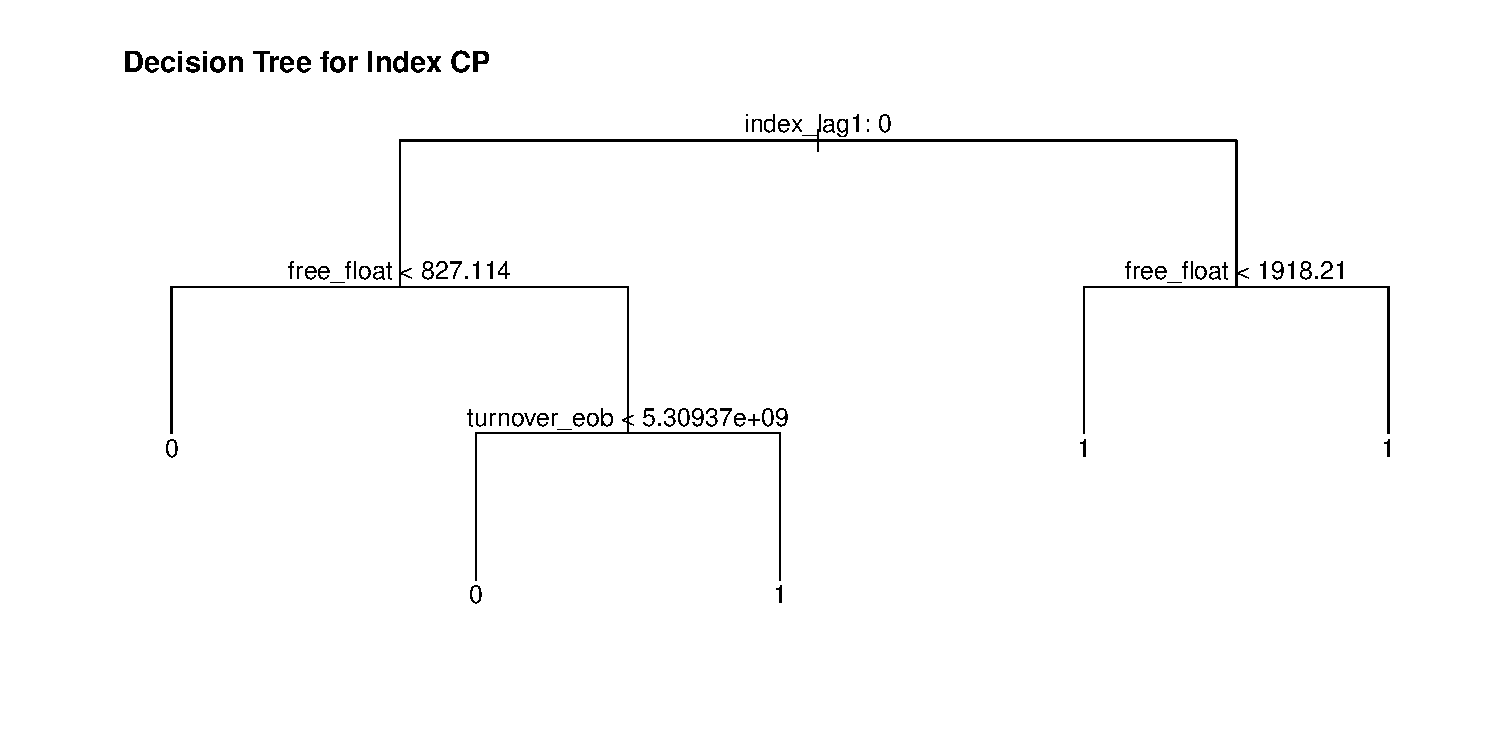
\includegraphics[width=\linewidth]{images/decision_tree_plot.pdf}
%     \caption{Decision Tree}
%     \label{fig:decision-tree}
% \end{figure}
% \vspace{-1cm}

% \textit{Bagged Trees:}
% Decision trees notoriousely suffer from high variance, as altering the variables used in the nodes may alter the resulting predictions. One powerful idea to leviate this is to repeatedly grow several decision trees, and thereafter aggregate their predictions. This process is called bagging. If the independent observations of decision trees are $Z_1,...,Z_n$ with variance $\sigma^2$, we find the mean of the bagging $\overline{Z}$ and corresponding variance $\sigma^2/n$. Averaging over several decision trees will in this effect reduce the variance between its predictions. Reiterating over the same training set $B$ times, one can find the average of predictions in the following formula: 
% \begin{equation}
%     \hat{f}_{bag}(x)=\frac{1}{B}\sum_{b=1}^{B}\hat{f}^{*b}(x)
% \end{equation}
% Looking at the performance of such bagged trees, the out-of-bag error estimate is commonly used.  
% \begin{equation}
% Out\ Of\ Bag\ Error = 1 - \frac{1}{N}\sum_{i=1}^{N} I(y_i = \hat{y}_{i}^{OOB})
% \end{equation}

% \textcite{breiman-random-forest}.
% \textit{Random Forest:}
% The power of Decision Trees are extracted when generating multiple such decision rule sets, and then taking the average decision rules for each branch. When generating many trees, we are facing a different model, called Random Forest (RF). This method is the baseline for any Decision Tree Model, and in this thesis we are going to focus on eXtreme Gradient Boosting, which is an iteration of the Random Forest. Random Forest is viewed as a further improvement to the bagged decision trees. The model decorrelates the individual trees even more, lowering prediction variance further. For each split in a tree, only a random sample of \textit{m} predictors from the predictor variables are considered. An approximation is to use $m\approx\sqrt{p}$ predictor variables for each split. Decorrelation comes from only considering a subset of predictors, where this reduces the usage of strong predictors, making sure the individual trees look more different. Using $m=p$ yields the same results as a bagged tree.  
% \begin{equation}
%     Gini\ Importance = \sum_{t \in T} p(t) \cdot \Delta i(s, t)
% \end{equation}

% \textit{Boosted Trees:}
% Boosted trees deviate from the previous tree models in terms of trees being sequential, rather than averaged across several non-sequential trees. In other words, with boosted trees, each new decision tree is grown using information from the previous trees. In opposition to fitting single large decision trees, boosted trees learn slowly by fitting using current residuals rather than the predicted variable \textit{Y}. The general equation for updating the model after each iteration follows:
% \begin{equation}
% F_{m}(x) = F_{m-1}(x) + \nu \cdot \gamma_{m} \cdot h_{m}(x)
% \end{equation}



%%%%%%%%% arbitrage



If the index effect is a structural event of abnormal returns compared to CAPM, it may be considered an arbitrage opportunity \parencite{shleifer-the-limits-of-arbitrage}.  



\textcite{shleifer-the-limits-of-arbitrage}.
The concept of arbitrage in finance can be defined as the simultaneous long/short trade of essentially similar securities in two different markets with advantageous price differences. We find papers proclaiming the index effect to exist, which in that case gives clear inconsistent with the EMH. In that sense, the index effect may be labelled an arbitrage opportunity. Shleifer point out that textbook arbitrages requires no capital and zero risk, but in reality most arbitrage opportunities may require both large amounts of capital and may entail high risk. 

\textcite{ross-arbitrage}.
The 1976 paper from Ross communicates the arbitrage pricing theory (APT). APT is an alternative to the earlier mentioned CAPM, being somewhat harder to implement. Below is the APT, where $E(R_i)$ is the expected return, $R_f$ is the risk-free rate, $\beta$ is the sensitivity of an asset in relation to the specified factor, and $RP$ is the risk premium of a specific factor. 
\begin{align}
    E(R_i)=R_f \\
    &+\beta_{i1} \cdot RP_1 \\
    &+ \beta_{i2} \cdot RP_2 \\
    &+ ... \\
    &+ \beta_{kn} \cdot RP_n
\end{align}






% \begin{table*}[b]
% \centering\small
% \begin{tabularx}{\textwidth}{Xlllllllllllll}
% \hline
% {Model} & {Accuracy} & {Kappa} & {Sensitivity} & {Specificity} & {PPV} & {NPV} & {TN} & {FP} & {FN} & {TP} & {F} & {N} \\
% \hline
% glm30   & 0.947 & 0.885 & 0.953 & 0.937 & 0.964 & 0.917 & 2707 & 100 & 134 & 1479 & 0.927 & 100 \\
% glm60   & 0.947 & 0.885 & 0.953 & 0.936 & 0.964 & 0.917 & 2688 & 100 & 133 & 1469 & 0.927 &  84 \\
% glm100  & 0.947 & 0.885 & 0.954 & 0.934 & 0.963 & 0.920 & 2675 & 104 & 128 & 1464 & 0.927 &  71 \\
% xgbb60  & 0.939 & 0.868 & 0.937 & 0.943 & 0.967 & 0.892 & 2642 &  90 & 179 & 1479 & 0.917 & 182 \\
% xgbb30  & 0.937 & 0.864 & 0.937 & 0.937 & 0.964 & 0.892 & 2661 &  99 & 180 & 1480 & 0.914 & 187 \\
% xgbb100 & 0.935 & 0.860 & 0.936 & 0.932 & 0.961 & 0.891 & 2625 & 107 & 178 & 1461 & 0.911 & 182 \\
% xgbc30  & 0.913 & 0.814 & 0.913 & 0.915 & 0.951 & 0.853 & 2593 & 135 & 248 & 1444 & 0.883 & 345 \\
% xgbc100 & 0.911 & 0.809 & 0.914 & 0.906 & 0.945 & 0.854 & 2561 & 148 & 242 & 1420 & 0.879 & 341 \\
% xgbc60  & 0.908 & 0.803 & 0.914 & 0.899 & 0.942 & 0.853 & 2578 & 159 & 243 & 1410 & 0.875 & 363 \\
% \hline
% \end{tabularx}
% \label{tab:my_label}
% \end{table*}



\begin{figure}[ht]
    \centering
    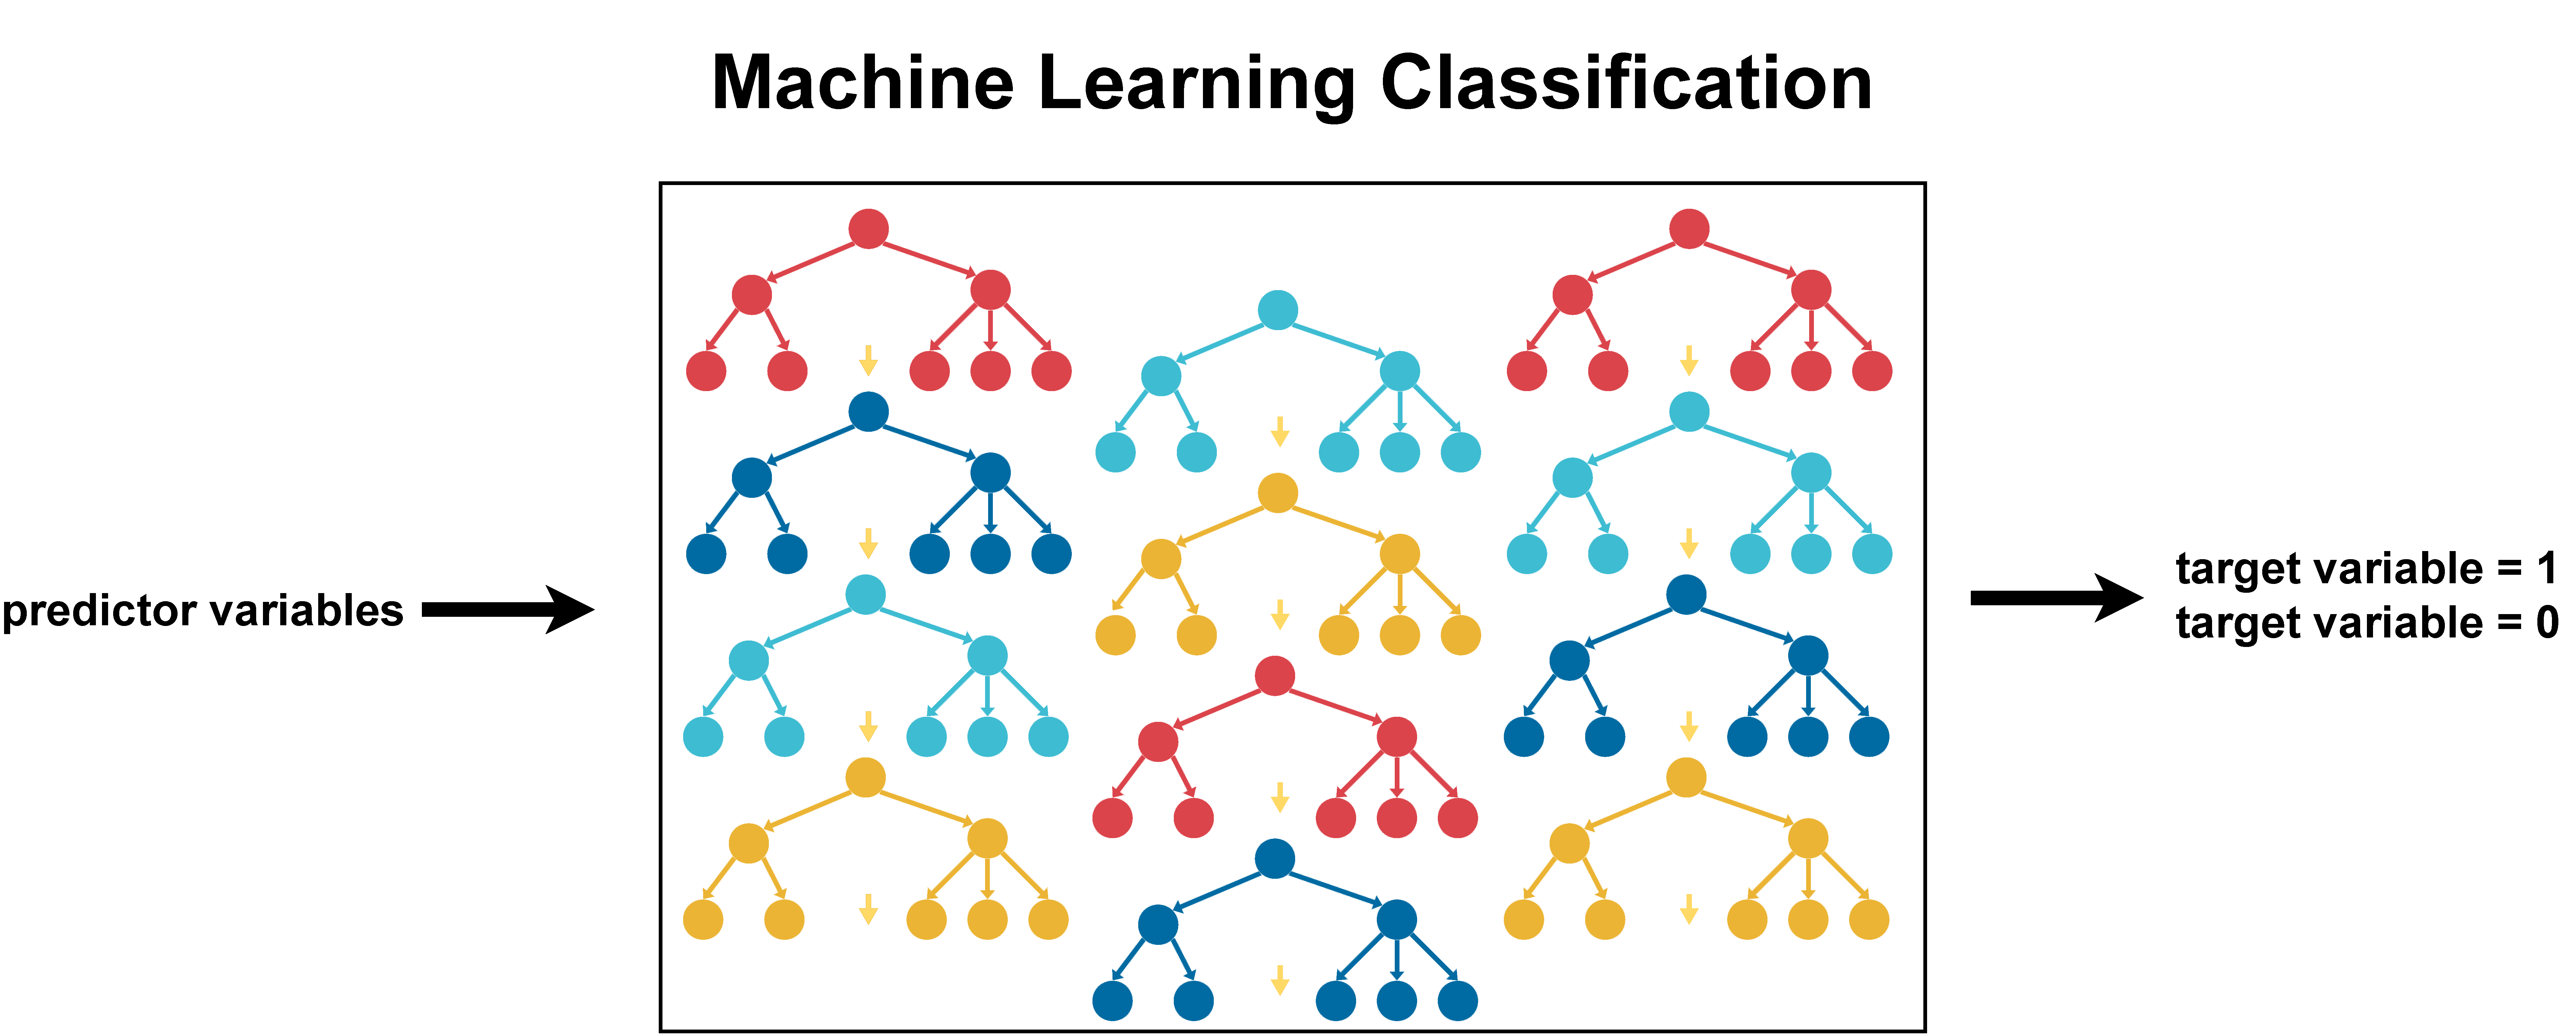
\includegraphics[width=\linewidth]{images/machine-learning-framework.drawio (6).pdf}
    \vspace{1em}
    \caption{The Machine Learning Classification Algorithm}
    \label{fig:machine-learning-classification-algorithm}
\end{figure}



\begin{table}[H]
\centering
\begin{tabularx}{\textwidth}{Xlllllll}
\hline
Model          & $R_p$  & $\sigma_p$ & SR & $\alpha$  & $\beta$  & TE & IR \\
\hline
OSEBX    & 0.0120  & 0.0538 & 0.201  & 0.0120 & 1.000 & 0.0000         & NaN               \\
\hline
XGBC30L  & 0.0147  & 0.0597 & 0.227  & 0.0147 & 1.030 & 0.0224         & 0.124             \\
GLM30L   & 0.0127  & 0.0638 & 0.180  & 0.0127 & 1.090 & 0.0256         & 0.0272            \\
XGBC30   & 0.0114  & 0.0542 & 0.189  & 0.0114 & 0.880 & 0.0271         & -0.0201           \\
XGBB30L  & 0.0147  & 0.0643 & 0.210  & 0.0147 & 1.040 & 0.0316         & 0.0847            \\
XGBB30   & 0.0131  & 0.0615 & 0.194  & 0.0131 & 0.967 & 0.0327         & 0.0346            \\
XGBC60L  & 0.0152  & 0.0616 & 0.227  & 0.0152 & 0.954 & 0.0340         & 0.0937            \\
XGBB60L  & 0.0113  & 0.0643 & 0.158  & 0.0113 & 0.938 & 0.0398         & -0.0158           \\
XGBC60   & 0.0102  & 0.0459 & 0.196  & 0.0102 & 0.525 & 0.0441         & -0.0411           \\
GLM30    & 0.0147  & 0.0659 & 0.206  & 0.0147 & 0.909 & 0.0442         & 0.0621            \\
XGBC100L & 0.0144  & 0.0553 & 0.240  & 0.0144 & 0.635 & 0.0476         & 0.0519            \\
GLM60L   & 0.00881 & 0.0684 & 0.112  & 0.00881 & 0.860 & 0.0507        & -0.0622           \\
GLM100L  & 0.00419 & 0.0695 & 0.0434 & 0.00419 & 0.846 & 0.0534        & -0.147            \\
XGBB60   & 0.00820 & 0.0711 & 0.0988 & 0.00820 & 0.828 & 0.0561        & -0.0671           \\
XGBC100  & 0.0105  & 0.0501 & 0.186  & 0.0105 & 0.258 & 0.0623         & -0.0242           \\
XGBB100L & 0.0135  & 0.0754 & 0.163  & 0.0135 & 0.721 & 0.0661         & 0.0223            \\
XGBB100  & 0.00690 & 0.0644 & 0.0891 & 0.00690 & 0.376 & 0.0696       & -0.0727           \\
GLM60    & 0.0136  & 0.0741 & 0.168  & 0.0136 & 0.357 & 0.0791         & 0.0208            \\
GLM100   & 0.0156  & 0.0783 & 0.184  & 0.0156 & 0.282 & 0.0856         & 0.0419            \\
\hline
\end{tabularx}
\caption{Performance of the Trading Strategies}
\label{tab:performance-trading-return-sigma-sharpe-alpha-beta-te-ir}
\end{table}



\begin{figure}[H]
    \centering
    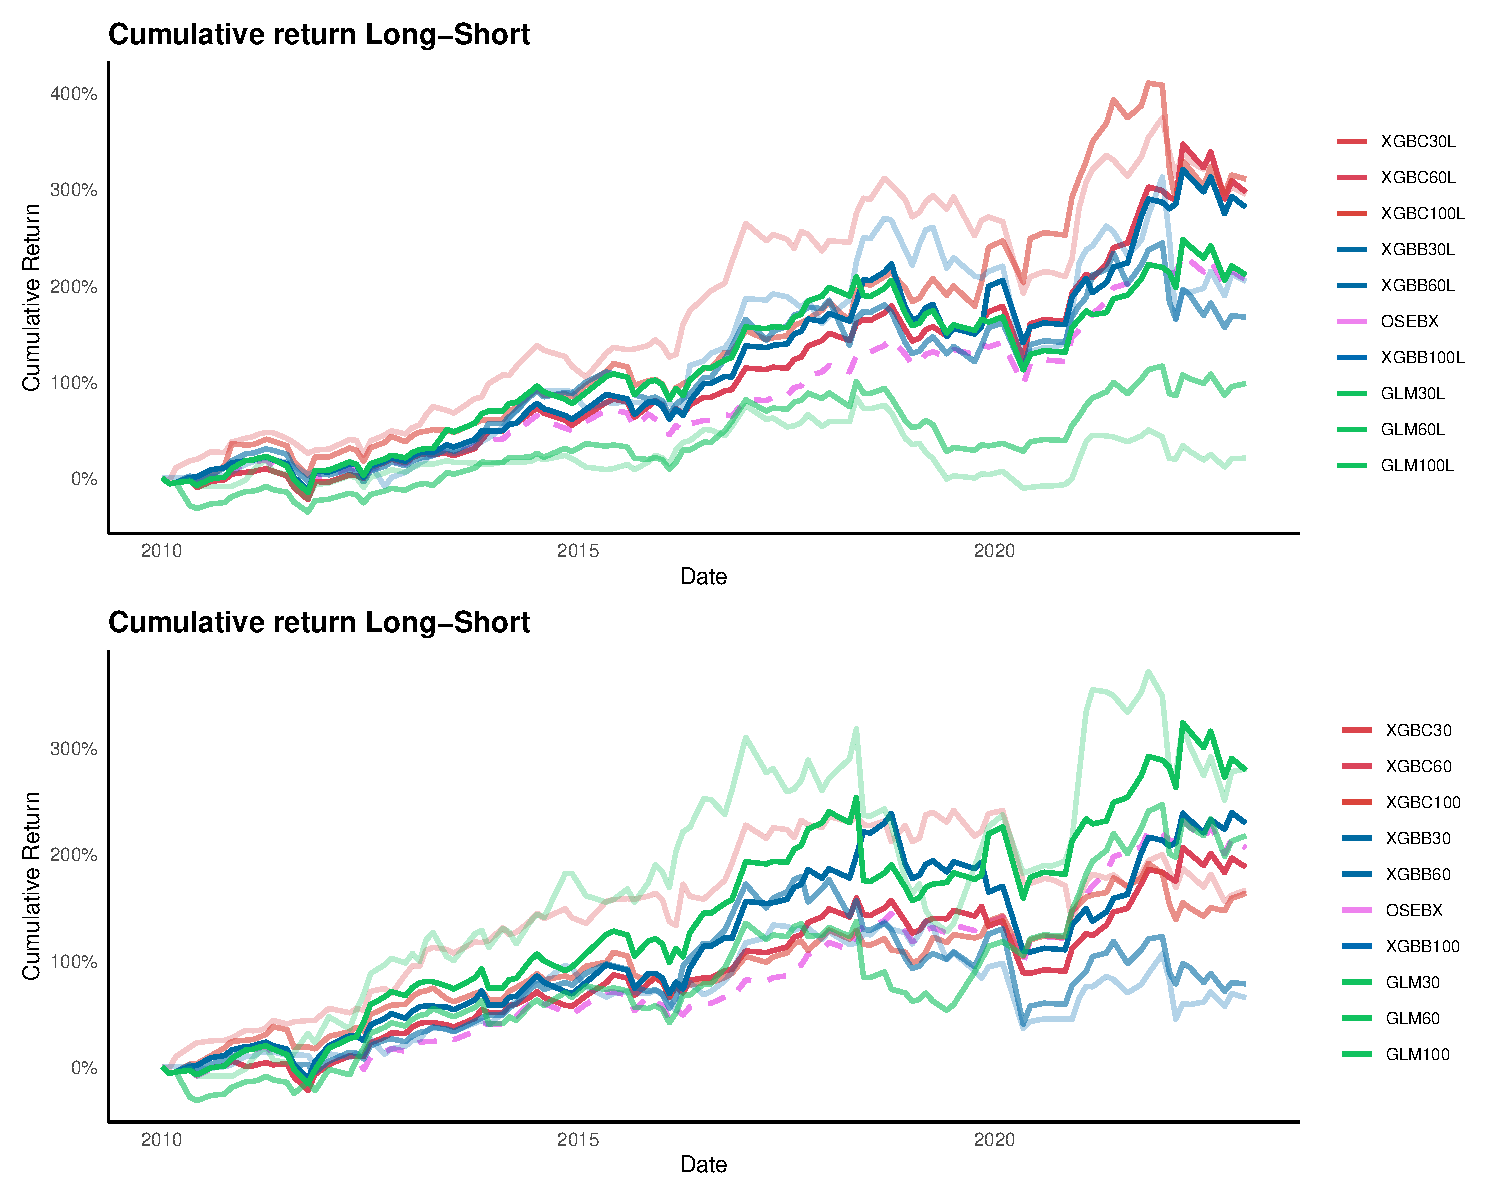
\includegraphics[width=\textwidth]{images/combined_plot.pdf}
    \caption{Combined Plot}
    \label{fig:combined-plot}
\end{figure}



\begin{table}[H]
\centering
\begin{tabular}{rrrrr}
\hline
Portfolio & Intercept ($\alpha$) & SMB & HML & UMD \\ 
\hline
GLM30  & .0139 & .0024 & .1078 & -.1782 \\ 
GLM100 & .0096 & .1999 & -.0106 & -.0425 \\ 
XGBB30 & .0134 & .0042 & .1668 & -.1890 \\ 
XGBB60 & .0070 & .0701 & .1637 & -.0634 \\ 
XGBB100& .0025 & .2224 & .0623 & -.0168 \\ 
XGBC30 & .0118 & .0147 & .1293 & -.1798 \\ 
XGBC60 & .0096 & -.0083 & .0697 & -.1065 \\ 
XGBC100& .0074 & -.0191 & .0385 & .0104 \\ 
\hline
\end{tabular}
\vspace{1em}
\caption{FF3 with Carhart for long-short portfolios}
\label{tab:famafrench-trading-long-short}
\end{table}

[OPPDATERT FIGUR OM FAMA FRENCH HER]

\begin{table}[H]
\centering
\begin{tabular}{rrrrr}
\hline
Portfolio & Intercept ($\alpha$) & SMB & HML & UMD \\
\hline
GLM30L  & .0119 & .1030 & .1663 & -.2076 \\ 
GLM60L  & .0083 & .1448 & .1256 & -.1840 \\ 
GLM100L & .0025 & .3002 & .0768 & -.1601 \\ 
XGBB30L & .0134 & .1176 & .1697 & -.2219 \\ 
XGBB60L & .0096 & .1919 & .1615 & -.1748 \\ 
XGBB100L& .0080 & .3503 & .1409 & -.1366 \\ 
XGBC30L & .0128 & .1247 & .1466 & -.1951 \\ 
XGBC60L & .0126 & .1648 & .0930 & -.2199 \\ 
XGBC100L& .0101 & .3008 & .1145 & -.1878 \\ 
\hline
\end{tabular}
\vspace{1em}
\caption{FF3 with Carhart for long-only portfolios}
\label{tab:famafrench-trading-long-only}
\end{table}



\texttt{trading\_status}
\begin{lstlisting}
    =@BQL(A2; "(#traded_days/" & F2 & ")*100"; "#px=px_last(dates=range(" &@BQL.DATE(D2) & "," &@BQL.DATE(E2) & "))"; "#traded_days=count(matches(#px,#px!=NA)).value"; "#total_days=count(#px().date).value")
\end{lstlisting}

\texttt{turnover}
\begin{lstlisting}
    =@BQL(A2;" #tot";"#high=sum(first(group(sort(turnover(dates=range(" &@BQL.DATE(C2) & "," &@BQL.DATE(E2) & ")),order=desc)),12)), #sum=sum(Group(turnover(dates=range(" &@BQL.DATE(C2) & "," &@BQL.DATE(E2) & ")))), #tot = #sum - #high")
\end{lstlisting}

\texttt{icb\_supersector}
\begin{lstlisting}
    =BDP(A2;"icb_supersector_name")
\end{lstlisting}

\texttt{free\_float}
\begin{lstlisting}
    =BDH(A2;"cur_mkt_cap";E2)*BDH(A2;"eqy_free_float_pct";E2)%
\end{lstlisting}



\subsubsection{GLM in R}
\begin{lstlisting}[language=R]
glm1 <- 
    glm(y~x1+x2+x3, 
    family=binomial(link="logit"),data)
\end{lstlisting}

\subsubsection{XGBoost in R}
\begin{lstlisting}[language=R]
xgboost1 <- 
   xgboost(data=data,label=label,max_depth,nthread,nrounds,
   objective="binary:logistic")
\end{lstlisting}

\begin{lstlisting}[language=R]
logregobj <- function(preds, dtrain) {
   labels <- getinfo(dtrain, "label")
   preds <- 1 / (1 + exp(-preds))
   grad <- preds - labels
   hess <- preds * (1 - preds)
   return(list(grad = grad, hess = hess))
}
\end{lstlisting}

\begin{lstlisting}[language=R]
logregobj <- function(preds, dtrain) {
   vec <- c()
   lag <- attr(dtrain, 'test')
   y <- getinfo(dtrain, "label")
   p <- 1 / (1 + exp(-preds))
   y_pred <- ifelse(p >= 0.5, 1, 0)
   b <- -1000000
   grad <- ifelse(y_pred == lag,
                  -b*(y-p),
                  p - y)
   hess <- ifelse(y_pred == lag,
                 (b)*p * (1-p),
                 p * (1-p))
   return(list(grad = grad, hess = hess))
}
\end{lstlisting}




\begin{table}[H]
\centering
\begin{tabular}{lllll}
\hline
Portfolio & Intercept ($\alpha$) & SMB & HML & UMD \\
\hline
GLM30L   & .0119 & .1030 & .1660 & -.2080 \\ 
GLM60L   & .0083 & .1450 & .1260 & -.1840 \\ 
GLM100L  & .0025 & .3000 & .0768 & -.1600 \\ 
XGBB30L  & .0134 & .1180 & .1700 & -.2220 \\ 
XGBB60L  & .0096 & .1920 & .1620 & -.1750 \\ 
XGBB100L & .0080 & .3500 & .1410 & -.1370 \\ 
XGBC30L  & .0126 & .1010 & .1570 & -.2170 \\ 
XGBC60L  & \cellcolor{lightlightgreen} .0136 & .1930 & .1260 & -.2490 \\ 
XGBC100L & .0106 & .2830 & .1280 & -.1690 \\ 
\hline
\end{tabular}
\vspace{1em}
\caption{FF3 with Carhart for long-only portfolios}
\label{tab:new-famafrench-trading-long-only}
\end{table}

\begin{table}[H]
\centering
\begin{tabular}{lllll}
\hline
Portfolio & Intercept ($\alpha$) & SMB & HML & UMD \\ 
\hline
GLM30  & \cellcolor{lightlightgreen} .0139 & .0024 & .1078 & -.1782 \\ 
GLM60  & .0108 & .0546 & .0287 & -.0819 \\ 
GLM100 & .0096 & .2000 & -.0106 & -.0425 \\ 
XGBB30 & .0134 & .0042 & .1670 & -.1890 \\ 
XGBB60 & .0070 & .0701 & .1640 & -.0634 \\ 
XGBB100& .0025 & .2224 & .0623 & -.0168 \\ 
XGBC30 & .0129 & .0103 & .1320 & -.2090 \\ 
XGBC60 & .0091 & .0494 & .0885 & -.0997 \\ 
XGBC100& .0031 & .0297 & -.0371 & .0738 \\ 
OSEBX  & .0118 & .0874 & .1400 & -.2180 \\ 
\hline
\end{tabular}
\vspace{1em}
\caption{FF3 with Carhart for long-short portfolios}
\label{tab:new-famafrench-trading-long-short}
\end{table}



\begin{table}[H]
\centering
\vspace{1em}
\caption{CD, AD, and ED from 2006 to 2023}
\label{CD-AD-ED-2006-2023}
\begin{tabular}{llll}
\hline
 & CD & AD & ED \\ 
\hline
1 & 2023-02-17 & 2023-03-08 & 2023-03-17 \\ 
2 & 2022-08-19 & 2022-09-07 & 2022-09-16 \\ 
3 & 2022-02-18 & 2022-03-09 & 2022-03-18 \\ 
4 & 2021-08-20 & 2021-09-08 & 2021-09-17 \\ 
5 & 2021-02-19 & 2021-03-10 & 2021-03-19 \\ 
6 & 2020-04-30 & 2020-05-12 & 2020-05-29 \\ 
7 & 2019-11-01 & 2019-11-08 & 2019-11-29 \\ 
8 & 2019-05-03 & 2019-05-09 & 2019-05-31 \\ 
9 & 2018-11-02 & 2018-11-09 & 2018-11-30 \\ 
10 & 2018-05-03 & 2018-05-09 & 2018-05-31 \\ 
11 & 2017-11-02 & 2017-11-10 & 2017-11-30 \\ 
12 & 2017-05-03 & 2017-05-05 & 2017-05-31 \\ 
13 & 2016-11-02 & 2016-11-10 & 2016-11-30 \\ 
14 & 2016-05-03 & 2016-05-12 & 2016-05-31 \\ 
15 & 2015-11-02 & 2015-11-12 & 2015-11-30 \\ 
16 & 2015-04-30 & 2015-05-13 & 2015-05-29 \\ 
17 & 2014-10-31 & 2014-11-13 & 2014-11-28 \\ 
\hline
\end{tabular}
\end{table}

\begin{table}[H]
\centering
\begin{tabular}{llll}
\hline
 & CD & AD & ED \\ 
\hline 
18 & 2014-05-02 & 2014-05-15 & 2014-05-30 \\ 
19 & 2013-11-01 & 2013-11-14 & 2013-11-29 \\ 
20 & 2013-05-03 & 2013-05-14 & 2013-05-31 \\ 
21 & 2012-11-02 & 2012-11-16 & 2012-11-30 \\ 
22 & 2012-05-03 & 2012-05-16 & 2012-05-31 \\ 
23 & 2011-11-02 & 2011-11-11 & 2011-11-30 \\ 
24 & 2011-05-03 & 2011-05-12 & 2011-05-31 \\ 
25 & 2010-11-02 & 2010-11-15 & 2010-11-30 \\ 
26 & 2010-05-03 & 2010-05-12 & 2010-05-31 \\ 
27 & 2009-11-02 & 2009-11-13 & 2009-11-30 \\ 
28 & 2009-04-30 & 2009-05-14 & 2009-05-29 \\ 
29 & 2008-12-02 & 2008-12-11 & 2008-12-30 \\ 
30 & 2008-06-02 & 2008-06-05 & 2008-06-30 \\ 
31 & 2007-11-30 & 2007-12-04 & 2007-12-30 \\ 
32 & 2007-06-01 & 2007-06-08 & 2007-06-29 \\ 
33 & 2006-12-01 & 2006-12-04 & 2006-12-29 \\ 
34 & 2006-06-02 & 2006-06-08 & 2006-06-30 \\ 
\hline
\end{tabular}
\end{table}



\begin{table}[H]
\centering
\begin{tabularx}{\textwidth}{Xlllllll}
\toprule
Portfolio    & $R_p$   & $\sigma_p$ & SR    & $\alpha$ & $\beta$ & TE     & IR \\
\midrule
OSEBX    & 0.0120  & 0.0538     & 0.200 & 0.0120   & 1.000   & 0.0000 & NaN \\
\midrule
XGBC60L  & \cellcolor{lightlightgreen} 0.0162  & 0.0651     & \cellcolor{lightlightgreen} 0.230 & \cellcolor{lightlightgreen} 0.0162   & 0.912   & 0.0430 & \cellcolor{lightlightgreen} 0.0979 \\
XGBC30L  & 0.0134  & 0.0574     & 0.212 & 0.0134   & 0.992   & 0.0211 & 0.0657 \\
XGBB30L  & 0.0147  & 0.0643     & 0.209 & 0.0147   & 1.040   & \cellcolor{lightlightgreen} 0.0316 & 0.0847 \\
XGBC30   & 0.0122  & 0.0532     & 0.207 & 0.0122   & 0.860   & 0.0270 & 0.00886 \\
GLM30    & 0.0147  & 0.0659     & 0.205 & 0.0147   & 0.909   & 0.0442 & 0.0621 \\
XGBC100L & 0.0158  & 0.0723     & 0.202 & 0.0158   & 0.851   & 0.0563 & 0.0681 \\
XGBB30   & 0.0131  & 0.0615     & 0.193 & 0.0131   & 0.967   & 0.0327 & 0.0346 \\
XGBC60   & 0.0107  & \cellcolor{lightlightgreen} 0.0503     & 0.188 & 0.0107   & 0.583   & 0.0451 & -0.0292 \\
GLM100   & 0.0156  & 0.0783     & 0.183 & 0.0156   & 0.282   & 0.0856 & 0.0419 \\
GLM30L   & 0.0127  & 0.0638     & 0.180 & 0.0127   & \cellcolor{lightlightgreen} 1.090   & 0.0256 & 0.0272 \\
GLM60    & 0.0136  & 0.0741     & 0.167 & 0.0136   & 0.357   & 0.0791 & 0.0208 \\
XGBB100L & 0.0135  & 0.0754     & 0.162 & 0.0135   & 0.721   & 0.0661 & 0.0223 \\
XGBB60L  & 0.0113  & 0.0643     & 0.157 & 0.0113   & 0.938   & 0.0398 & -0.0158 \\
XGBC100  & 0.00737 & 0.0530     & 0.116 & 0.00737  & \cellcolor{lightlightgreen} 0.171   & 0.0685 & -0.0670 \\
GLM60L   & 0.00881 & 0.0684     & 0.111 & 0.00881  & 0.860   & 0.0507 & -0.0622 \\
XGBB60   & 0.00820 & 0.0711     & 0.0982 & 0.00820 & 0.828   & 0.0561 & -0.0671 \\
XGBB100  & 0.00690 & 0.0644     & 0.0883 & 0.00690 & 0.376   & 0.0696 & -0.0727 \\
GLM100L  & 0.00419 & 0.0695     & 0.0428 & 0.00419 & 0.846   & 0.0534 & -0.147 \\
\bottomrule
\end{tabularx}
\vspace{1em}
\caption{Performance of the Trading Strategies}
\label{tab:new-performance-trading-return-sigma-sharpe-alpha-beta-te-ir}
\end{table}



\begin{table}[H]
\centering
\begin{tabularx}{\textwidth}{lXXXX}
\toprule
Portfolio & Intercept ($\alpha$) & SMB & HML & UMD \\
\midrule
GLM30L   & .0119 & .1030 & .1660 & -.2080 \\ 
GLM60L   & .0083 & .1450 & .1260 & -.1840 \\ 
GLM100L  & .0025 & .3000 & .0768 & -.1600 \\ 
XGBB30L  & .0134 & .1180 & .1700 & -.2220 \\ 
XGBB60L  & .0096 & .1920 & .1620 & -.1750 \\ 
XGBB100L & .0080 & .3500 & .1410 & -.1370 \\ 
XGBC30L  & .0126 & .1010 & .1570 & -.2170 \\ 
XGBC60L  & \cellcolor{lightlightgreen} .0136 & .1930 & .1260 & -.2490 \\ 
XGBC100L & .0106 & .2830 & .1280 & -.1690 \\ 
\bottomrule
\end{tabularx}
\vspace{1em}
\caption{FF3 with Carhart for long-only portfolios}
\label{tab:new-famafrench-trading-long-only}
\end{table}

The regression analysis for long-short trading strategies are shown in \autoref{tab:new-famafrench-trading-long-short}.

\begin{table}[H]
\centering
\begin{tabularx}{\textwidth}{lXXXX}
\toprule
Portfolio & Intercept ($\alpha$) & SMB & HML & UMD \\ 
\midrule
GLM30  & \cellcolor{lightlightgreen} .0139 & .0024 & .1078 & -.1782 \\ 
GLM60  & .0108 & .0546 & .0287 & -.0819 \\ 
GLM100 & .0096 & .2000 & -.0106 & -.0425 \\ 
XGBB30 & .0134 & .0042 & .1670 & -.1890 \\ 
XGBB60 & .0070 & .0701 & .1640 & -.0634 \\ 
XGBB100& .0025 & .2224 & .0623 & -.0168 \\ 
XGBC30 & .0129 & .0103 & .1320 & -.2090 \\ 
XGBC60 & .0091 & .0494 & .0885 & -.0997 \\ 
XGBC100& .0031 & .0297 & -.0371 & .0738 \\ 
OSEBX  & .0118 & .0874 & .1400 & -.2180 \\ 
\bottomrule
\end{tabularx}
\vspace{1em}
\caption{FF3 with Carhart for long-short portfolios}
\label{tab:new-famafrench-trading-long-short}
\end{table}




\begin{table}[H]
\centering
\begin{tabularx}{\textwidth}{lXXXX}
\toprule
Portfolio & Intercept ($\alpha$) & SMB & HML & UMD \\
\midrule
OSEBX  & .0118 & .0874 & .1400 & -.2180 \\
\midrule
GLM30L   & .0119 & .1030 & .1660 & -.2080 \\ 
GLM60L   & .0083 & .1450 & .1260 & -.1840 \\ 
GLM100L  & .0025 & .3000 & .0768 & -.1600 \\ 
XGBB30L  & \cellcolor{lightlightgreen} .0134 & .1180 & .1700 & -.2220 \\ 
XGBB60L  & .0096 & .1920 & .1620 & -.1750 \\ 
XGBB100L & .0080 & .3500 & .1410 & -.1370 \\ 
XGBC30L  & .0131 & .1010 & .1320 & -.2230 \\ 
XGBC60L  & .0104 & .1720 & .1090 & -.2250 \\ 
XGBC100L & .0088 & .2370 & .1050 & -.1550 \\ 
\bottomrule
\end{tabularx}
\vspace{1em}
\caption{FF3 with Carhart for Portfolios with "L" Suffix}
\label{tab:new-famafrench-trading-l-suffix}
\end{table}

\begin{table}[H]
\centering
\begin{tabularx}{\textwidth}{lXXXX}
\toprule
Portfolio & Intercept ($\alpha$) & SMB & HML & UMD \\
\midrule
OSEBX  & .0118 & .0874 & .1400 & -.2180 \\
\midrule
GLM30  & \cellcolor{lightlightgreen} .0139 & .0024 & .1078 & -.1782 \\ 
GLM60  & .0108 & .0546 & .0287 & -.0819 \\ 
GLM100 & .0096 & .2000 & -.0106 & -.0425 \\ 
XGBB30 & .0134 & .0042 & .1670 & -.1890 \\ 
XGBB60 & .0070 & .0701 & .1640 & -.0634 \\ 
XGBB100& .0025 & .2224 & .0623 & -.0168 \\ 
XGBC30 & .0129 & .0103 & .1320 & -.2090 \\ 
XGBC60 & .0091 & .0494 & .0885 & -.0997 \\ 
XGBC100& .0031 & .0297 & -.0371 & .0738 \\ 
\bottomrule
\end{tabularx}
\vspace{1em}
\caption{FF3 with Carhart for Portfolios without "L" Suffix}
\label{tab:new-famafrench-trading-no-l-suffix}
\end{table}



\begin{table}[H]
\centering
\begin{tabularx}{\textwidth}{Xlllllll}
\toprule
Portfolio & $R_p$ & $\sigma_p$ & SR & $\alpha$ & $\beta$ & TE & IR \\
\midrule
OSEBX & 0.0120 & 0.0538 & 0.200 & 0.0000 & 1.000 & 0.0000 & NaN \\
\midrule
XGBC30 & 0.0135 & 0.0555 & \cellcolor{lightlightgreen}0.221 & 0.00223 & 0.934 & 0.0821 & 0.0642 \\
XGBC30L & 0.0144 & 0.0599 & 0.220 & 0.00226 & 1.02 & 0.0843 & 0.0998 \\
XGBB30L & 0.0147 & 0.0643 & 0.209 & 0.00225 & 1.04 & 0.110 & 0.0847 \\
GLM30 & 0.0147 & 0.0659 & 0.205 & 0.00374 & 0.909 & 0.154 & 0.0621 \\
XGBB30 & 0.0131 & 0.0615 & 0.193 & 0.00149 & 0.967 & 0.114 & 0.0346 \\
GLM100 & 0.0156 & 0.0783 & 0.183 & 0.0113 & 0.282 & 0.298 & 0.0419 \\
GLM30L & 0.0127 & 0.0638 & 0.180 & -0.000243 & 1.09 & 0.0889 & 0.0272 \\
XGBC100L & 0.0122 & 0.0650 & 0.169 & 0.00364 & 0.685 & 0.194 & 0.00451 \\
GLM60 & 0.0136 & 0.0741 & 0.167 & 0.00856 & 0.357 & 0.275 & 0.0208 \\
XGBC60L & 0.0119 & 0.0645 & 0.165 & -0.000107 & 1.00 & 0.122 & -0.00230 \\
XGBB100L & 0.0135 & 0.0754 & 0.162 & 0.00448 & 0.721 & 0.230 & 0.0223 \\
XGBB60L & 0.0113 & 0.0643 & 0.157 & 0.0000374 & 0.938 & 0.138 & -0.0158 \\
XGBC100 & 0.00841 & 0.0541 & 0.133 & 0.00284 & 0.405 & 0.204 & -0.0605 \\
XGBC60 & 0.00871 & 0.0573 & 0.131 & -0.000446 & 0.738 & 0.151 & -0.0748 \\
GLM60L & 0.00881 & 0.0684 & 0.111 & -0.00166 & 0.860 & 0.176 & -0.0622 \\
XGBB60 & 0.00820 & 0.0711 & 0.0982 & -0.00192 & 0.828 & 0.195 & -0.0671 \\
XGBB100 & 0.00690 & 0.0644 & 0.0883 & 0.00164 & 0.376 & 0.242 & -0.0727 \\
GLM100L & 0.00419 & 0.0695 & 0.0428 & -0.00613 & 0.846 & 0.184 & -0.147 \\
\bottomrule
\end{tabularx}
\vspace{1em}
\caption{Performance of the Trading Strategies}
\label{tab:new-performance-trading-return-sigma-sharpe-alpha-beta-te-ir}
\end{table}



\begin{table}[!htbp] \centering 
  \caption{FF3 (with Carhart) for Selected Long-Only Regression Trading Strategies} 
  \vspace{1em}
  \label{table:trading-ff3-selected-long-only-part1} 
\begin{tabularx}{\textwidth}{lXXXXXX} 
\toprule 
 & OSEBX & XGBB30L & XGBC30L & GLM30L & XGBC100L & XGBC60L \\ 
\midrule
Constant ($\alpha$) & 0.016*** & \cellcolor{lightlightgreen}0.019*** & 0.018*** & 0.015*** & 0.016*** & 0.016*** \\ 
SMB & 0.031 & -0.005 & 0.031 & 0.082 & 0.030 & 0.171 \\ 
HML & 0.096 & 0.077 & 0.096 & 0.093 & 0.108 & 0.068 \\ 
UMD & 0.004 & 0.061 & 0.031 & 0.106 & -0.046 & 0.004 \\ 
\midrule 
Observations & 155 & 155 & 155 & 155 & 155 & 155 \\ 
R$^{2}$ & 0.010 & 0.009 & 0.010 & 0.020 & 0.011 & 0.014 \\ 
Adjusted R$^{2}$ & -0.009 & -0.011 & -0.010 & 0.00003 & -0.009 & -0.006 \\ 
Residual Std. Error & 0.054 & 0.064 & 0.060 & 0.063 & 0.059 & 0.063 \\ 
F Statistic & 0.520 & 0.459 & 0.505 & 1.002 & 0.549 & 0.708 \\ 
\bottomrule 
\textit{Note:} & \multicolumn{6}{r}{$^{*}$p$<$0.05; $^{**}$p$<$0.01; $^{***}$p$<$0.001} \\ 
\end{tabularx} 
\end{table} 

\begin{table}[!htbp] \centering 
  \caption{FF3 (with Carhart) for Selected Long-Short Regression Trading Strategies} 
  \vspace{1em}
  \label{table:trading-ff3-selected-long-short-part2} 
\begin{tabularx}{\textwidth}{lXXXXXX} 
\toprule
 & OSEBX & GLM100 & XGBC30 & XGBB30 & XGBC60 & XGBC100 \\ 
\midrule
Constant ($\alpha$) & 0.016*** & 0.012* & \cellcolor{lightlightgreen}0.019*** & 0.018*** & 0.011** & 0.014*** \\ 
SMB & 0.031 & 0.238 & -0.012 & -0.042 & 0.147 & -0.011 \\ 
HML & 0.096 & -0.032 & 0.116 & 0.128 & 0.089 & 0.065 \\ 
UMD & 0.004 & 0.023 & -0.003 & 0.013 & -0.070 & -0.108 \\ 
\midrule 
Observations & 155 & 155 & 155 & 155 & 155 & 155 \\ 
R$^{2}$ & 0.010 & 0.018 & 0.014 & 0.015 & 0.021 & 0.016 \\ 
Adjusted R$^{2}$ & -0.009 & -0.002 & -0.006 & -0.004 & 0.001 & -0.003 \\ 
Residual Std. Error & 0.054 & 0.075 & 0.056 & 0.063 & 0.055 & 0.051 \\ 
F Statistic & 0.520 & 0.908 & 0.717 & 0.785 & 1.060 & 0.842 \\ 
\bottomrule
\textit{Note:} & \multicolumn{6}{r}{$^{*}$p$<$0.05; $^{**}$p$<$0.01; $^{***}$p$<$0.001} \\ 
\end{tabularx} 
\end{table} 




\begin{table}[H] 
\centering 
  \caption{FF3 (with Carhart) for Long-Only Enhanced Index Strategies} 
  \vspace{1em}
  \label{table:enhanced-ff3-selected-long-only} 
\begin{tabularx}{\textwidth}{lXXXXXX} 
\toprule
 & OSEBX & GLM100L & XGBB30L & XGBC30L & XGBC60L & XGBC100L \\ 
\midrule
Constant ($\alpha$) & \cellcolor{lightlightgreen}0.016*** & 0.014*** & \cellcolor{lightlightgreen}0.016*** & 0.015*** & \cellcolor{lightlightgreen}0.016*** & 0.015*** \\ 
SMB & 0.031 & 0.054 & 0.028 & 0.047 & 0.025 & 0.031 \\ 
HML & 0.096 & 0.100 & 0.095 & 0.099 & 0.096 & 0.097 \\ 
UMD & 0.004 & 0.010 & 0.010 & -0.0003 & -0.0002 & 0.007 \\ 
\midrule 
Observations & 155 & 155 & 155 & 155 & 155 & 155 \\ 
R$^{2}$ & 0.010 & 0.012 & 0.011 & 0.011 & 0.011 & 0.010 \\ 
Adjusted R$^{2}$ & -0.009 & -0.008 & -0.009 & -0.009 & -0.009 & -0.009 \\ 
Residual Std. Error & 0.054 & 0.054 & 0.052 & 0.054 & 0.052 & 0.054 \\ 
F Statistic & 0.520 & 0.605 & 0.553 & 0.512 & 0.564 & 0.539 \\ 
\bottomrule
\textit{Note:} & \multicolumn{6}{r}{$^{*}$p$<$0.05; $^{**}$p$<$0.01; $^{***}$p$<$0.001} \\ 
\end{tabularx} 
\end{table}


\begin{table}[H] 
\centering 
  \caption{FF3 (with Carhart) for Long-Short Enhanced Index Strategies} 
  \vspace{1em}
  \label{table:enhanced-ff3-selected-long-short} 
\begin{tabularx}{\textwidth}{lXXXXXX} 
\toprule 
 & OSEBX & GLM30 & XGBB30 & XGBC30 & XGBC60 & XGBC100 \\ 
\midrule
Constant ($\alpha$) & \cellcolor{lightlightgreen}0.016*** & 0.015*** & 0.015*** & \cellcolor{lightlightgreen}0.016*** & 0.015*** & \cellcolor{lightlightgreen}0.016*** \\ 
SMB & 0.031 & 0.035 & 0.053 & 0.063 & 0.023 & 0.049 \\ 
HML & 0.096 & 0.092 & 0.097 & 0.081 & 0.100 & 0.102 \\ 
UMD & 0.004 & 0.007 & -0.006 & 0.006 & 0.005 & -0.010 \\ 
\midrule 
Observations & 155 & 155 & 155 & 155 & 155 & 155 \\ 
R$^{2}$ & 0.010 & 0.012 & 0.010 & 0.011 & 0.012 & 0.011 \\ 
Adjusted R$^{2}$ & -0.009 & -0.010 & -0.008 & -0.010 & -0.009 & -0.008 \\ 
Residual Std. Error & 0.054 & 0.054 & 0.052 & 0.050 & 0.054 & 0.053 \\ 
F Statistic & 0.520 & 0.484 & 0.588 & 0.509 & 0.558 & 0.613 \\ 
\bottomrule 
\textit{Note:} & \multicolumn{6}{r}{$^{*}$p$<$0.05; $^{**}$p$<$0.01; $^{***}$p$<$0.001} \\ 
\end{tabularx} 
\end{table}



\begin{sidewaystable}
\centering 
\caption{Fama-French Regression for All Long-Short Regression Trading Strategies}
\vspace{1em}
\label{table:models_without_L-all}
\begin{tabularx}{\textwidth}{lXXXXXXXXXX} 
\toprule
 & OSEBX & GLM30 & GLM60 & GLM100 & XGBB30 & XGBB60 & XGBB100 & XGBC30 & XGBC60 & XGBC100 \\ 
\midrule
 Constant ($\alpha$) & 0.0118$^{**}$ & 0.0139$^{**}$ & 0.0108 & 0.0096 & 0.0134$^{**}$ & 0.0070 & 0.0025 & 0.0132$^{***}$ & 0.0086$^{*}$ & 0.0050 \\ 
 SMB & 0.0874 & 0.0024 & 0.0546 & 0.1999 & 0.0042 & 0.0701 & 0.2224$^{*}$ & 0.0294 & 0.0664 & 0.1813$^{*}$ \\ 
 HML & 0.1397$^{*}$ & 0.1078 & 0.0287 & $-$0.0106 & 0.1668$^{*}$ & 0.1637$^{*}$ & 0.0623 & 0.1229 & 0.1248 & 0.0612 \\ 
 UMD & $-$0.2183$^{***}$ & $-$0.1782$^{*}$ & $-$0.0819 & $-$0.0425 & $-$0.1890$^{**}$ & $-$0.0634 & $-$0.0168 & $-$0.1998$^{**}$ & $-$0.1576$^{*}$ & $-$0.0819 \\ 
\midrule
 Observations & 155 & 155 & 155 & 155 & 155 & 155 & 155 & 155 & 155 & 155 \\ 
 R$^{2}$ & 0.0972 & 0.0433 & 0.0061 & 0.0147 & 0.0692 & 0.0303 & 0.0311 & 0.0747 & 0.0525 & 0.0411 \\ 
 Adjusted R$^{2}$ & 0.0792 & 0.0243 & $-$0.0137 & $-$0.0048 & 0.0507 & 0.0110 & 0.0118 & 0.0563 & 0.0337 & 0.0220 \\ 
 Residual Std. Error & 0.0422 & 0.0509 & 0.0663 & 0.0713 & 0.0476 & 0.0535 & 0.0516 & 0.0431 & 0.0451 & 0.0430 \\ 
 F Statistic & 5.4170$^{**}$ & 2.2801 & 0.3068 & 0.7530 & 3.7397$^{*}$ & 1.5724 & 1.6143 & 4.0644$^{**}$ & 2.7882$^{*}$ & 2.1569 \\ 
\bottomrule
\textit{Note:} & \multicolumn{10}{r}{$^{*}$p$<$0.05; $^{**}$p$<$0.01; $^{***}$p$<$0.001} \\ 
\end{tabularx} 
\end{sidewaystable} 

\begin{sidewaystable}
\centering 
  \caption{Fama-French Regression for All Long-Only Regression Trading Strategies} 
  \vspace{1em}
  \label{table:models_with_L-all} 
\begin{tabularx}{\textwidth}{lXXXXXXXXXX} 
\toprule
 & OSEBXL & GLM30L & GLM60L & GLM100L & XGBB30L & XGBB60L & XGBB100L & XGBC30L & XGBC60L & XGBC100L \\ 
\midrule
 Constant ($\alpha$) & 0.0118$^{**}$ & 0.0119$^{**}$ & 0.0083 & 0.0025 & 0.0134$^{**}$ & 0.0096$^{*}$ & 0.0080 & 0.0131$^{**}$ & 0.0104$^{*}$ & 0.0088 \\ 
 SMB & 0.0874 & 0.1030 & 0.1448 & 0.3002$^{*}$ & 0.1176 & 0.1919 & 0.3503$^{*}$ & 0.1097 & 0.1715 & 0.2369$^{*}$ \\ 
 HML & 0.1397$^{*}$ & 0.1663$^{*}$ & 0.1256 & 0.0768 & 0.1697$^{*}$ & 0.1615$^{*}$ & 0.1409 & 0.1316$^{*}$ & 0.1094 & 0.1048 \\ 
 UMD & $-$0.2183$^{***}$ & $-$0.2076$^{**}$ & $-$0.1840$^{*}$ & $-$0.1601 & $-$0.2219$^{**}$ & $-$0.1748$^{*}$ & $-$0.1366 & $-$0.2233$^{***}$ & $-$0.2251$^{**}$ & $-$0.1553 \\ 
\midrule
 Observations & 155 & 155 & 155 & 155 & 155 & 155 & 155 & 155 & 155 & 155 \\ 
 R$^{2}$ & 0.0972 & 0.0884 & 0.0485 & 0.0620 & 0.0897 & 0.0688 & 0.0585 & 0.0927 & 0.0777 & 0.0502 \\ 
 Adjusted R$^{2}$ & 0.0792 & 0.0703 & 0.0295 & 0.0433 & 0.0716 & 0.0503 & 0.0398 & 0.0747 & 0.0593 & 0.0313 \\ 
 Residual Std. Error & 0.0422 & 0.0455 & 0.0567 & 0.0596 & 0.0479 & 0.0521 & 0.0678 & 0.0443 & 0.0513 & 0.0586 \\ 
 F Statistic & 5.4170$^{**}$ & 4.8819$^{**}$ & 2.5630 & 3.3245$^{*}$ & 4.9600$^{**}$ & 3.7202$^{*}$ & 3.1256$^{*}$ & 5.1428$^{**}$ & 4.2388$^{**}$ & 2.6599 \\ 
\bottomrule 
\textit{Note:} & \multicolumn{10}{r}{$^{*}$p$<$0.05; $^{**}$p$<$0.01; $^{***}$p$<$0.001} \\ 
\end{tabularx} 
\end{sidewaystable} 

\begin{sidewaystable}
\centering 
  \caption{Fama-French Regression for All Long-Only Enhanced Index} 
  \vspace{1em}
  \label{table:enhanced-models_with_L-all} 
\begin{tabularx}{\textwidth}{lXXXXXXXXXX} 
\toprule
 & OSEBX & GLM30L & GLM60L & GLM100L & XGBB30L & XGBB60L & XGBB100L & XGBC30L & XGBC60L & XGBC100L \\ 
\midrule
 Constant ($\alpha$) & 0.016*** & 0.015*** & 0.014*** & 0.008 & 0.019*** & 0.014*** & 0.015*** & 0.018*** & 0.018*** & 0.016*** \\ 
 SMB & 0.031 & 0.082 & 0.311** & 0.324** & -0.005 & 0.152 & -0.052 & 0.031 & 0.171 & 0.030 \\ 
 HML & 0.096 & 0.093 & 0.130 & 0.040 & 0.077 & 0.113 & 0.094 & 0.096 & 0.068 & 0.108 \\ 
 UMD & 0.004 & 0.106 & 0.035 & 0.064 & 0.061 & -0.034 & -0.035 & 0.031 & 0.004 & -0.046 \\ 
\midrule
 Observations & 155 & 155 & 155 & 155 & 155 & 155 & 155 & 155 & 155 & 155 \\ 
 R$^{2}$ & 0.010 & 0.020 & 0.044 & 0.040 & 0.009 & 0.018 & 0.007 & 0.010 & 0.014 & 0.011 \\ 
 Adjusted R$^{2}$ & -0.009 & 0.00003 & 0.025 & 0.021 & -0.011 & -0.002 & -0.013 & -0.010 & -0.006 & -0.009 \\ 
 Residual Std. Error & 0.054 & 0.063 & 0.064 & 0.066 & 0.064 & 0.062 & 0.071 & 0.060 & 0.063 & 0.059 \\ 
 F Statistic & 0.520 & 1.002 & 2.336* & 2.092 & 0.459 & 0.912 & 0.354 & 0.505 & 0.708 & 0.549 \\ 
\bottomrule 
\textit{Note:} & \multicolumn{10}{r}{$^{*}$p$<$0.05; $^{**}$p$<$0.01; $^{***}$p$<$0.001} \\ 
\end{tabularx} 
\end{sidewaystable}

\begin{sidewaystable}
\centering 
\caption{Fama-French Regression for All Long-Short Enhanced Index}
\vspace{1em}
\label{table:enhanced-models_without_L-all}
\begin{tabularx}{\textwidth}{lXXXXXXXXXX} 
\toprule
 & OSEBX & GLM30 & GLM60 & GLM100 & XGBB30 & XGBB60 & XGBB100 & XGBC30 & XGBC60 & XGBC100 \\ 
\midrule
 Constant ($\alpha$) & 0.016*** & 0.020*** & 0.014** & 0.012* & 0.018*** & 0.013** & 0.013** & 0.019*** & 0.011** & 0.014*** \\ 
 SMB & 0.031 & 0.069 & 0.278* & 0.238 & -0.042 & 0.174 & -0.068 & -0.012 & 0.147 & -0.011 \\ 
 HML & 0.096 & 0.064 & 0.094 & -0.032 & 0.128 & 0.125 & 0.064 & 0.116 & 0.089 & 0.065 \\ 
 UMD & 0.004 & 0.015 & -0.085 & 0.023 & 0.013 & -0.128 & -0.101 & -0.003 & -0.070 & -0.108 \\ 
\midrule
 Observations & 155 & 155 & 155 & 155 & 155 & 155 & 155 & 155 & 155 & 155 \\ 
 R$^{2}$ & 0.010 & 0.004 & 0.027 & 0.018 & 0.015 & 0.027 & 0.012 & 0.014 & 0.021 & 0.016 \\ 
 Adjusted R$^{2}$ & -0.009 & -0.016 & 0.008 & -0.002 & -0.004 & 0.008 & -0.007 & -0.006 & 0.001 & -0.003 \\ 
 Residual Std. Error & 0.054 & 0.067 & 0.075 & 0.075 & 0.063 & 0.067 & 0.061 & 0.056 & 0.055 & 0.051 \\ 
 F Statistic & 0.520 & 0.216 & 1.413 & 0.908 & 0.785 & 1.412 & 0.632 & 0.717 & 1.060 & 0.842 \\ 
\bottomrule
\textit{Note:} & \multicolumn{10}{r}{$^{*}$p$<$0.05; $^{**}$p$<$0.01; $^{***}$p$<$0.001} \\ 
\end{tabularx} 
\end{sidewaystable}


Trading versus Enhanced. 

Interest-rate on short-position. 

TE. 

Discussion on strategy design, considering factors like trading frequency, long-short positioning, and prediction strictness. Challenges related to liquidity and potential delistings. Exploration of optimal cut-off dates and sensitivity analysis regarding financial costs.


NB! Important discussion here: Why do we have to pay interest rate to ourself, if we can short stocks we already own? Remember, we can only short stocks that are included in our passive investment (being OSEBX), so in a practical sence, we would only sell those stocks. However, by doing so we remove our alternative cost of actually holding those shares. Therefore, we decide to simulate the long-short portfolios using a interest rate on short positions. Also, there would be no garanty that we would have a sufficient number of shares avalible in our passive fund, so it would be a dangerous assumption to not simulate for a short-posisition interest rate.




\begin{table}[H]
\centering
\begin{tabularx}{\textwidth}{Xlllllll}
\toprule
Portfolio & $R_p$ & $\sigma_p$ & SR & $\alpha$ & $\beta$ & TE & IR \\
\midrule
OSEBX & 0.0120 & 0.0538 & 0.200 & 0.0000 & 1.000 & 0.0000 & NaN \\
\midrule
GLM100 & 0.0120 & \cellcolor{lightlightgreen}0.0499 & \cellcolor{lightlightgreen}0.216 & \cellcolor{lightlightgreen}0.00103 & 0.906 & 0.0408 & 0.00186 \\
GLM60 & 0.0119 & 0.0511 & 0.208 & 0.000526 & 0.941 & 0.0260 & -0.0148 \\
GLM30 & \cellcolor{lightlightgreen}0.0122 & 0.0536 & 0.205 & 0.000317 & 0.990 & \cellcolor{lightlightgreen}0.0192 & 0.0377 \\
XGBC30 & 0.0121 & 0.0535 & 0.204 & 0.000212 & 0.993 & \cellcolor{lightlightgreen}0.00892 & \cellcolor{lightlightgreen}0.0533 \\
XGBC100 & 0.0115 & 0.0506 & 0.203 & 0.000224 & 0.936 & 0.0206 & -0.0783 \\
XGBB30 & 0.0120 & 0.0538 & 0.201 & 0.000099 & 0.998 & \cellcolor{lightlightgreen}0.0125 & 0.0200 \\
XGBB100 & 0.0114 & 0.0505 & 0.201 & 0.000135 & 0.930 & 0.0245 & -0.0867 \\
XGBC60 & 0.0116 & 0.0526 & 0.198 & -0.000074 & 0.974 & \cellcolor{lightlightgreen}0.0143 & -0.0867 \\
XGBB60 & 0.0115 & 0.0529 & 0.195 & -0.000194 & 0.977 & 0.0208 & -0.0731 \\
\midrule
XGBC30L & \cellcolor{lightlightgreen}0.0122 & 0.0540 & \cellcolor{lightlightgreen}0.204 & 0.000219 & 1.00 & \cellcolor{lightlightgreen}0.00983 & \cellcolor{lightlightgreen}0.0856 \\
XGBC100L & 0.0119 & \cellcolor{lightlightgreen}0.0523 & 0.203 & 0.000237 & 0.967 & \cellcolor{lightlightgreen}0.0197 & -0.0209 \\
XGBB30L & \cellcolor{lightlightgreen}0.0122 & 0.0542 & 0.203 & 0.000195 & 1.01 & \cellcolor{lightlightgreen}0.0122 & 0.0713 \\
XGBB100L & 0.0119 & 0.0528 & 0.203 & \cellcolor{lightlightgreen}0.000258 & 0.971 & 0.0265 & -0.00677 \\
GLM30L & 0.0120 & 0.0544 & 0.199 & -0.000054 & 1.01 & \cellcolor{lightlightgreen}0.00970 & 0.0159 \\
XGBC60L & 0.0119 & 0.0540 & 0.198 & -0.000063 & 1.00 & \cellcolor{lightlightgreen}0.0127 & -0.0177 \\
XGBB60L & 0.0118 & 0.0536 & 0.198 & -0.000051 & 0.993 & \cellcolor{lightlightgreen}0.0156 & -0.0288 \\
GLM60L & 0.0116 & 0.0535 & 0.194 & -0.000253 & 0.990 & \cellcolor{lightlightgreen}0.0148 & -0.0847 \\
GLM100L & 0.0114 & 0.0533 & 0.190 & -0.000481 & 0.987 & \cellcolor{lightlightgreen}0.0131 & -0.164 \\
\bottomrule
\end{tabularx}
\vspace{1em}
\caption{CAPM Portfolio Performance for Enhanced Index Strategies using Monthly Returns}
\label{tab:new-performance-enhanced-index-return-sigma-sharpe-alpha-beta-te-ir}
\end{table}



\subsubsection{Fama-French}

Here we show \autoref{table:FAMA-FRENCH-LONG-SHORT-ENHANCED-FINAL} and \autoref{table:FAMA-FRENCH-LONG-ONLY-ENHANCED-FINAL}.

% LONG ONLY ENHANCED
\begin{table}[H] \centering 
  \caption{Fama-French Regression for Long-Short Enhanced Index Portfolios} 
  \label{table:FAMA-FRENCH-LONG-SHORT-ENHANCED-FINAL} 
\begin{tabularx}{\textwidth}{XXXXXXXXXXl} 
\\[-1.8ex]\hline 
\hline \\[-1.8ex] 
 & \multicolumn{10}{c}{\textit{Dependent variable:}} \\ 
\cline{2-11} 
\\[-1.8ex] 
 & \multicolumn{3}{c}{GLM} & \multicolumn{3}{c}{XGBB} & \multicolumn{3}{c}{XGBC} & \\
 \cline{2-11}
 \\[-1.8ex] 
 & 30 & 60 & 100 & 30 & 60 & 100 & 30 & 60 & 100 & OSEBX \\ 
 \cline{2-11} \\
 SMB & 0.089 & 0.091 & 0.101 & 0.091 & 0.098 & 0.118 & 0.090 & 0.096 & 0.104 & 0.087 \\ 
  & (0.086) & (0.086) & (0.085) & (0.086) & (0.086) & (0.084) & (0.085) & (0.086) & (0.085) & (0.086) \\ 
  & & & & & & & & & & \\ 
 HML & 0.143$^{**}$ & 0.139$^{**}$ & 0.137$^{**}$ & 0.144$^{**}$ & 0.143$^{**}$ & 0.141$^{**}$ & 0.139$^{**}$ & 0.137$^{**}$ & 0.135$^{**}$ & 0.140$^{**}$ \\ 
  & (0.062) & (0.062) & (0.061) & (0.062) & (0.062) & (0.061) & (0.062) & (0.062) & (0.061) & (0.062) \\ 
  & & & & & & & & & & \\ 
 UMD & $-$0.217$^{***}$ & $-$0.215$^{***}$ & $-$0.214$^{***}$ & $-$0.219$^{***}$ & $-$0.213$^{***}$ & $-$0.210$^{***}$ & $-$0.219$^{***}$ & $-$0.219$^{***}$ & $-$0.212$^{***}$ & $-$0.218$^{***}$ \\ 
  & (0.061) & (0.062) & (0.061) & (0.061) & (0.061) & (0.060) & (0.061) & (0.062) & (0.061) & (0.061) \\ 
  & & & & & & & & & & \\ 
 $\alpha$ & 0.012$^{***}$ & 0.012$^{***}$ & 0.011$^{***}$ & 0.012$^{***}$ & 0.012$^{***}$ & 0.011$^{***}$ & 0.012$^{***}$ & 0.012$^{***}$ & 0.011$^{***}$ & 0.012$^{***}$ \\ 
  & (0.004) & (0.004) & (0.004) & (0.004) & (0.004) & (0.004) & (0.004) & (0.004) & (0.004) & (0.004) \\ 
  & & & & & & & & & & \\ 
\hline \\[-1.8ex] 
Obs & 155 & 155 & 155 & 155 & 155 & 155 & 155 & 155 & 155 & 155 \\ 
R$^{2}$ & 0.098 & 0.095 & 0.097 & 0.099 & 0.097 & 0.101 & 0.099 & 0.098 & 0.097 & 0.097 \\ 
R$^{2}$_{adj} & 0.080 & 0.077 & 0.079 & 0.081 & 0.079 & 0.083 & 0.081 & 0.080 & 0.079 & 0.079 \\ 
RSE & 0.042 & 0.042 & 0.042 & 0.042 & 0.042 & 0.041 & 0.042 & 0.042 & 0.042 & 0.042 \\ 
(df=151)  & & & & & & & & & & \\
F_{score}  & {\footnotesize 5.448$^{***}$ & 5.295$^{***}$ & 5.404$^{***}$ & 5.541$^{***}$ & 5.383$^{***}$ & 5.644$^{***}$ & 5.514$^{***}$ & 5.441$^{***}$ & 5.397$^{***}$ & 5.417$^{***}$} \\ 
(df=3;151) & & & & & & & & & & \\
\hline 
\hline \\[-1.8ex] 
\textit{Note:}  & \multicolumn{10}{r}{$^{*}$p$<$0.1; $^{**}$p$<$0.05; $^{***}$p$<$0.01} \\ 
\end{tabularx} 
\end{table} 


% LONG SHORT ENHANCED
\begin{table}[H] \centering 
  \caption{Fama-French Regression for Long-Short Enhanced Index Portfolios} 
  \label{table:FAMA-FRENCH-LONG-ONLY-ENHANCED-FINAL} 
\begin{tabularx}{\textwidth}{XXXXXXXXXXl} 
\\[-1.8ex]\hline 
\hline \\[-1.8ex] 
 & \multicolumn{10}{c}{\textit{Dependent variable:}} \\ 
\cline{2-11} 
\\[-1.8ex] 
& \multicolumn{3}{c}{GLM L} & \multicolumn{3}{c}{XGBB L} & \multicolumn{3}{c}{XGBC L} & \\
\cline{2-11}
\\[-1.8ex] 
& 30 & 60 & 100 & 30 & 60 & 100 & 30 & 60 & 100 & OSEBX \\ 
\cline{2-11} \\
 SMB & 0.077 & 0.084 & 0.100 & 0.079 & 0.084 & 0.097 & 0.081 & 0.085 & 0.096 & 0.087 \\ 
  & (0.085) & (0.086) & (0.084) & (0.085) & (0.084) & (0.082) & (0.085) & (0.084) & (0.082) & (0.086) \\ 
  & & & & & & & & & & \\ 
 HML & 0.136$^{**}$ & 0.130$^{**}$ & 0.121$^{**}$ & 0.143$^{**}$ & 0.143$^{**}$ & 0.136$^{**}$ & 0.138$^{**}$ & 0.139$^{**}$ & 0.133$^{**}$ & 0.140$^{**}$ \\ 
  & (0.061) & (0.062) & (0.061) & (0.062) & (0.060) & (0.059) & (0.061) & (0.061) & (0.059) & (0.062) \\ 
  & & & & & & & & & & \\ 
 UMD & $-$0.213$^{***}$ & $-$0.205$^{***}$ & $-$0.192$^{***}$ & $-$0.215$^{***}$ & $-$0.202$^{***}$ & $-$0.201$^{***}$ & $-$0.216$^{***}$ & $-$0.212$^{***}$ & $-$0.206$^{***}$ & $-$0.218$^{***}$ \\ 
  & (0.061) & (0.061) & (0.060) & (0.061) & (0.060) & (0.058) & (0.061) & (0.060) & (0.059) & (0.061) \\ 
  & & & & & & & & & & \\ 
 $\alpha$ & 0.012$^{***}$ & 0.012$^{***}$ & 0.011$^{***}$ & 0.012$^{***}$ & 0.011$^{***}$ & 0.011$^{***}$ & 0.012$^{***}$ & 0.012$^{***}$ & 0.011$^{***}$ & 0.012$^{***}$ \\ 
  & (0.004) & (0.004) & (0.004) & (0.004) & (0.004) & (0.004) & (0.004) & (0.004) & (0.004) & (0.004) \\ 
  & & & & & & & & & & \\ 
\hline \\[-1.8ex] 
Obs & 155 & 155 & 155 & 155 & 155 & 155 & 155 & 155 & 155 & 155 \\ 
R$^{2}$ & 0.093 & 0.088 & 0.082 & 0.097 & 0.092 & 0.096 & 0.096 & 0.096 & 0.098 & 0.097 \\ 
R$^{2}$_{adj} & 0.075 & 0.069 & 0.064 & 0.079 & 0.074 & 0.078 & 0.079 & 0.079 & 0.080 & 0.079 \\ 
RSE & 0.042 & 0.042 & 0.041 & 0.042 & 0.041 & 0.040 & 0.042 & 0.041 & 0.040 & 0.042 \\ 
(df=151) & & & & & & & & & & \\
F_{score} & 5.163$^{***}$ & 4.827$^{***}$ & 4.508$^{***}$ & 5.376$^{***}$ & 5.128$^{***}$ & 5.361$^{***}$ & 5.373$^{***}$ & 5.375$^{***}$ & 5.460$^{***}$ & 5.417$^{***}$ \\ 
(df=3;151) & & & & & & & & & & \\
\hline 
\hline \\[-1.8ex] 
\textit{Note:}  & \multicolumn{10}{r}{$^{*}$p$<$0.1; $^{**}$p$<$0.05; $^{***}$p$<$0.01} \\ 
\end{tabularx} 
\end{table}  




\begin{table}[h]
\centering
\begin{tabular}{|l|rr|rr|rr|}
\toprule
& \multicolumn{2}{c|}{GLM} & \multicolumn{2}{c|}{XGBB} & \multicolumn{2}{c|}{XGBC} \\
\midrule
30 & 2707  & 134 & 2661 & 180 & 2563 & 278 \\
   & 100 & 1479 & 99 & 1480 & 113 & 1466 \\
\hline
60 & 2688  & 100 & 2642    & 90 & 2540   & 100 \\
   & 133  & 1469 & 179  & 1479 & 281  & 1469 \\
\hline
100 & 2675   & 104 & 2625   & 107 & 2538   & 107 \\
    & 128  & 1464 & 178  & 1461 & 265  & 1461 \\
\bottomrule
\end{tabular}
\vspace{1em}
\caption{Comparison of GLM, XGBB, and XGBC}
\label{confusion_matrix_result}
\end{table}







In the gradient boosting algorithm, we start with a data set $D$, the loss function $L$, a base learner $L_\Phi$, number of iterations $M$, and learning rate $\eta$. The algorithm is initialised in \autoref{initial-gradient} \parencite{ntnu-thesis-why-does-xgboost-win-every-machine-learning-competition}.

\vspace{-1em}
\begin{equation}
\label{initial-gradient}
    \hat{f}^{(0)}(x)=\hat{f}_o(x)=\hat{\theta}_0=\arg\min_{\theta}\sum_{i=1}^{n}L(y_i,\theta). 
\end{equation}

Next, the model algorithm iterate over $m=1,...,M$.


The gradient boosting algorithm output the model shown in \autoref{gradient-algorithm-output}. 

\begin{equation}
\label{gradient-algorithm-output}
    \hat{f}(x)\equiv\hat{f}^{M}(x)=\sum_{m=0}^M\hat{f}_{m}(x)
\end{equation}





\subsection{Tree Boosting Models}

Tree boosting have proven to be a widely used ML model \parencite{xgboost-a-scaleable-tree-boosting-system}, which is highly efficient in predictions \parencite{ntnu-thesis-why-does-xgboost-win-every-machine-learning-competition}. Tree boosting is in itself a general method for improving, "boosting", accuracy of a given ML algorithm \parencite{schapire-a-brief-introduction-to-boosting}. Compared to a Random Forest model, the tree boosting algorithm introduces a loss function, on which the predictions are evaluated for each iteration, and decision rules tweaked slightly to reduce the loss function \parencite{schapire-a-brief-introduction-to-boosting}. This is done contrary to Random Forest, which develop several single decision trees and average across them. The intuition behind a loss function in tree boosting models is in essence similar to the log-loss function in logistic regression \parencite{friedman-additive-logistic-regression}. In \autoref{from-decision-tree-to-xgboost} we illustrate the intuition behind a tree boosting system, where tree models are "boosted" over several iterations. 

\begin{figure}[H]
    \centering
    \vspace{1em}
    \begin{subfigure}{0.3\linewidth}
        \centering
        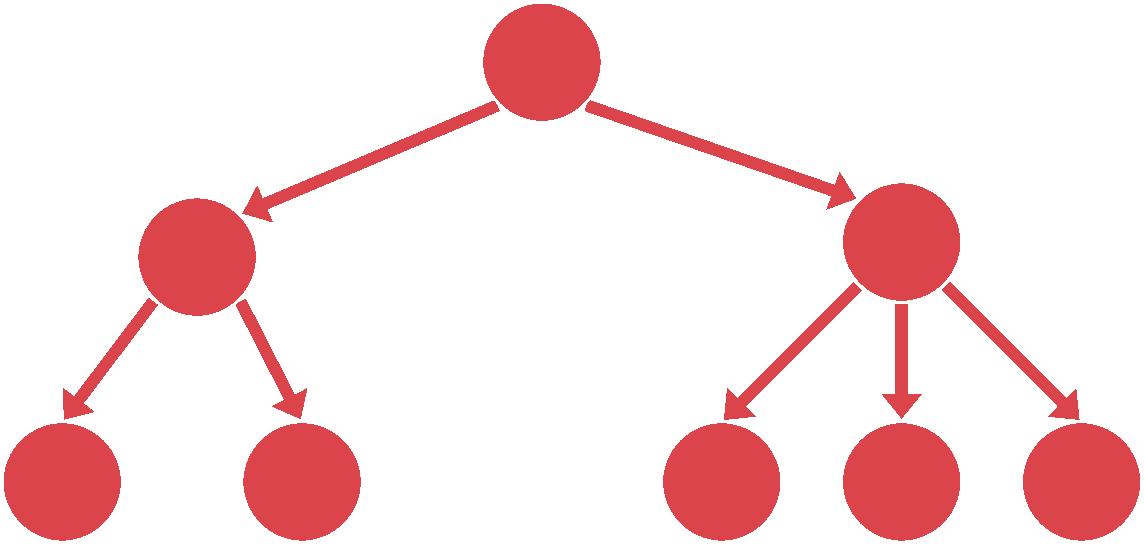
\includegraphics[width=\linewidth, height=\linewidth, keepaspectratio]{images/tree models.drawio.pdf}
        \caption{}
        \label{fig:draw-io-decision-tree}
    \end{subfigure}
    \hfill
    \begin{subfigure}{0.3\linewidth}
        \centering
        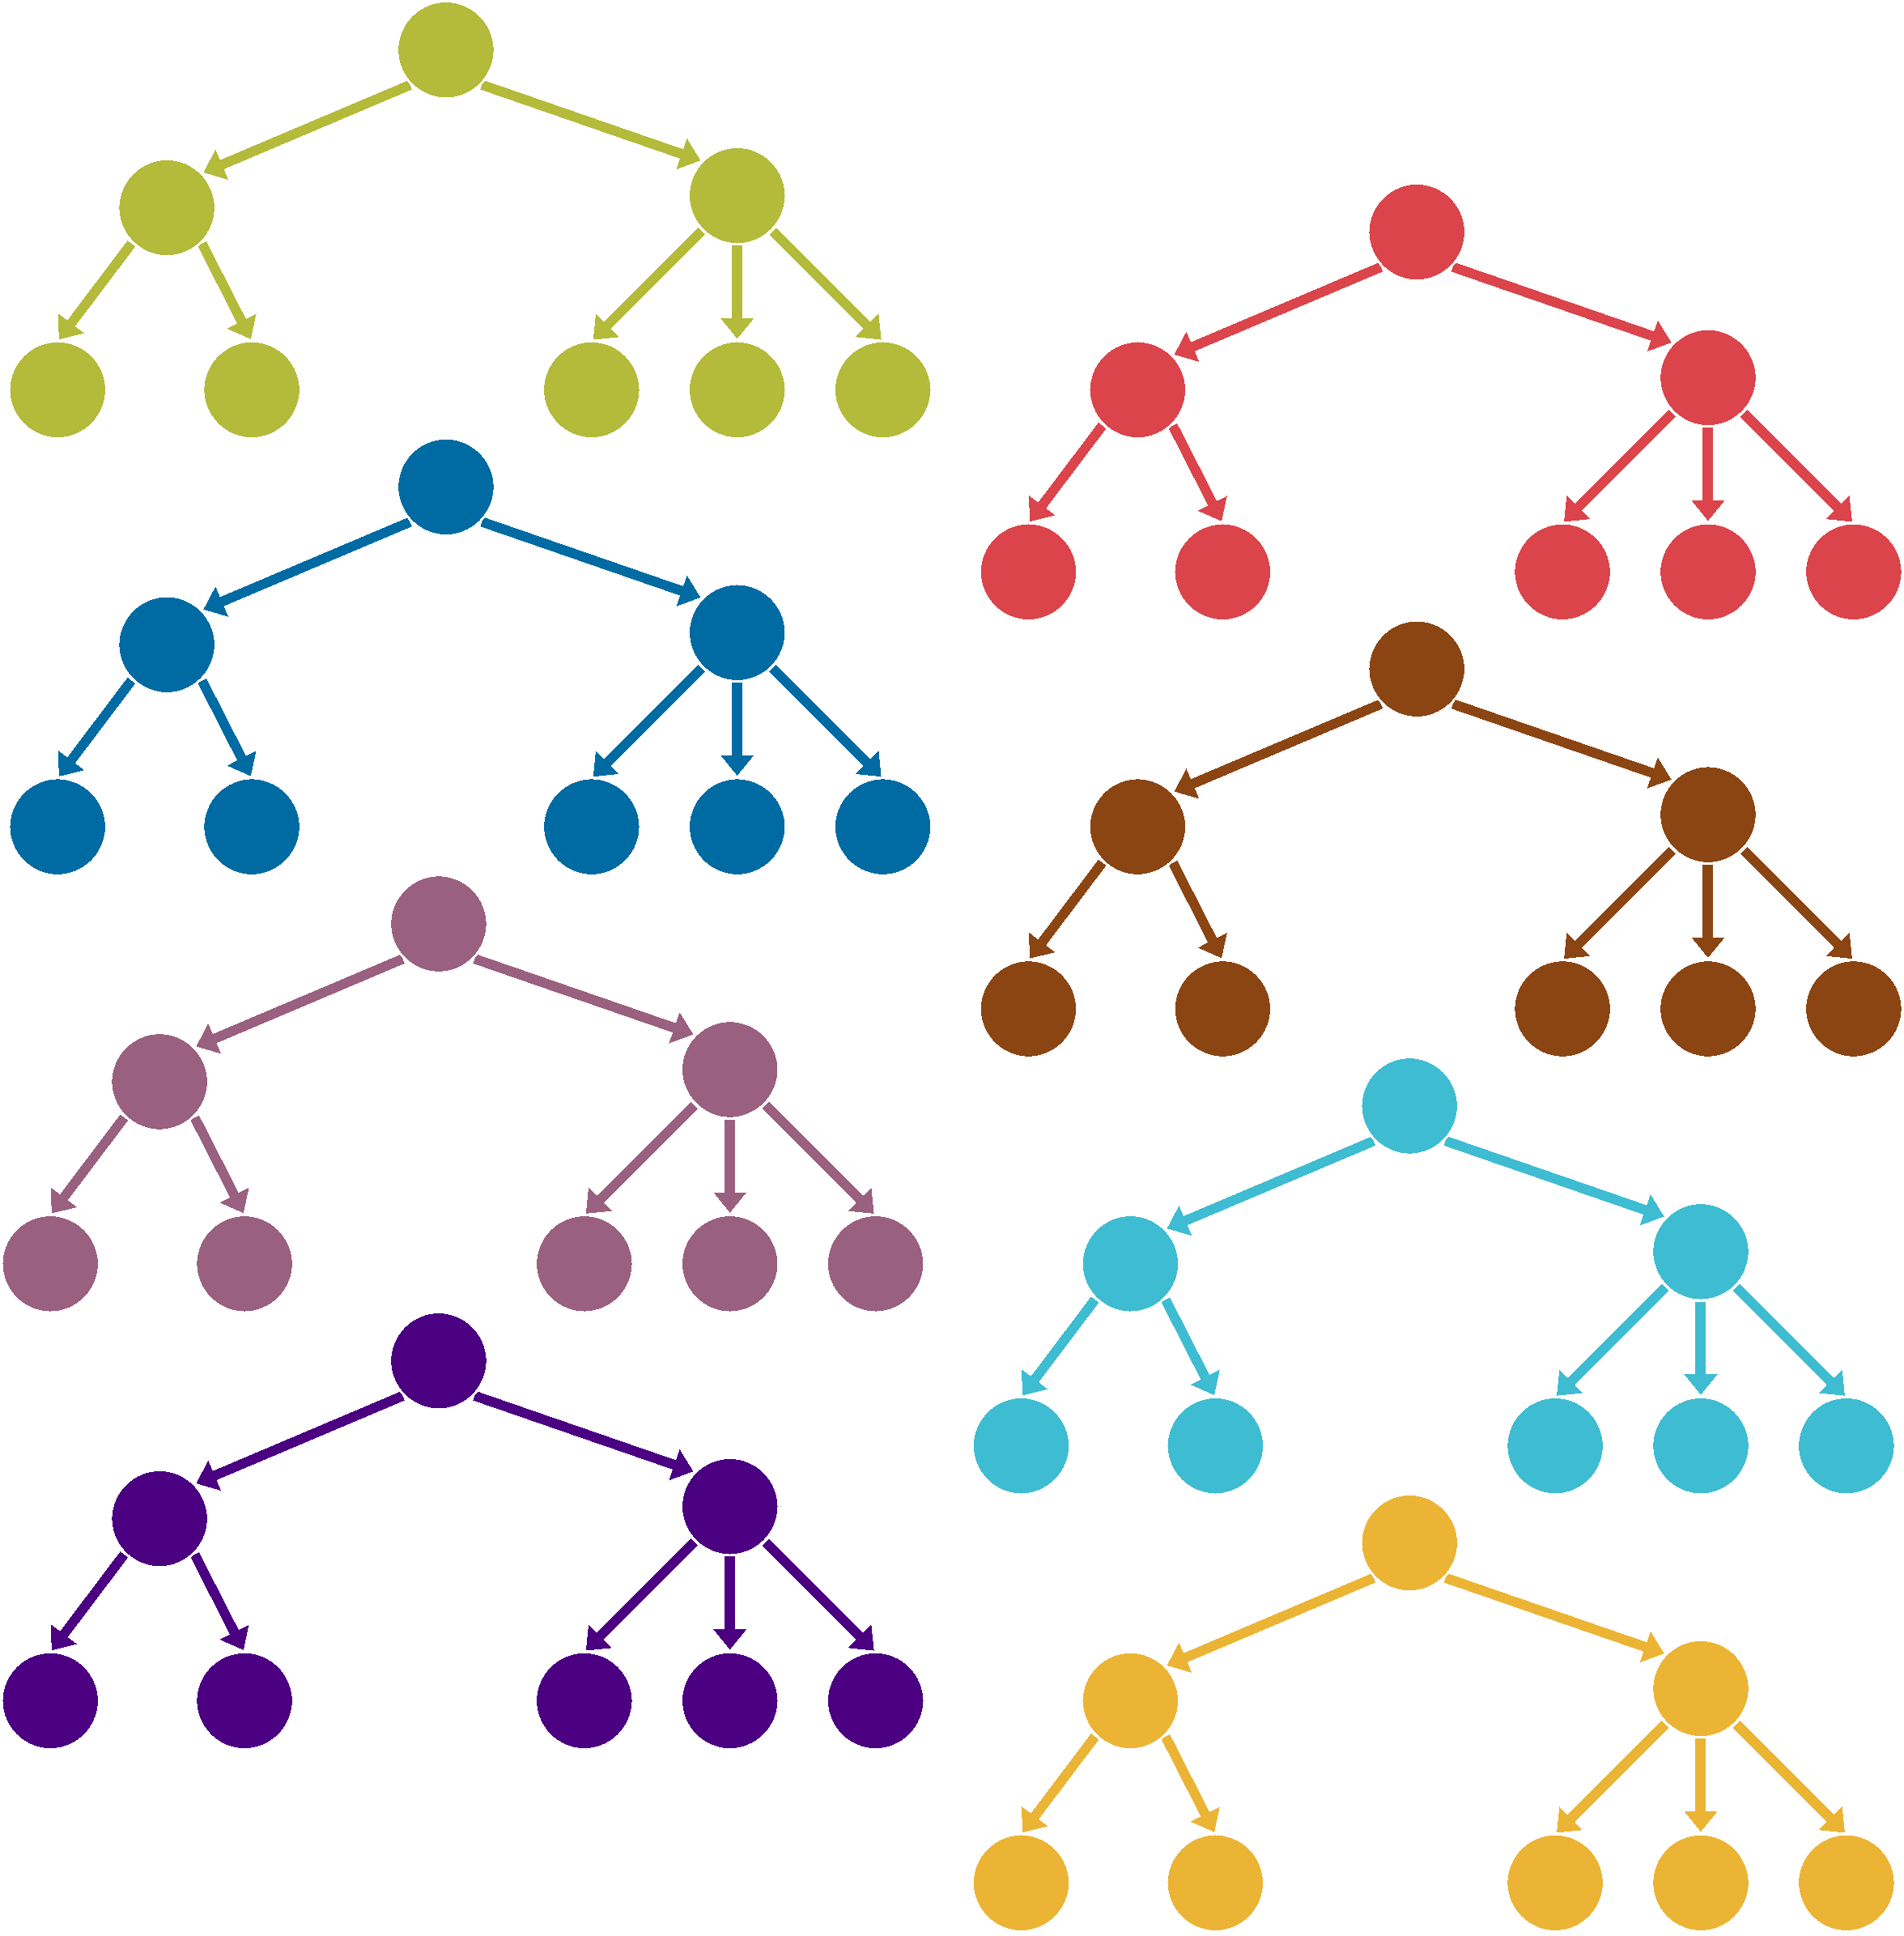
\includegraphics[width=\linewidth, height=\linewidth, keepaspectratio]{images/random forest diagram.drawio.pdf}
        \caption{}
        \label{fig:draw-io-random-forest}
    \end{subfigure}
    \hfill
    \begin{subfigure}{0.3\linewidth}
        \centering
        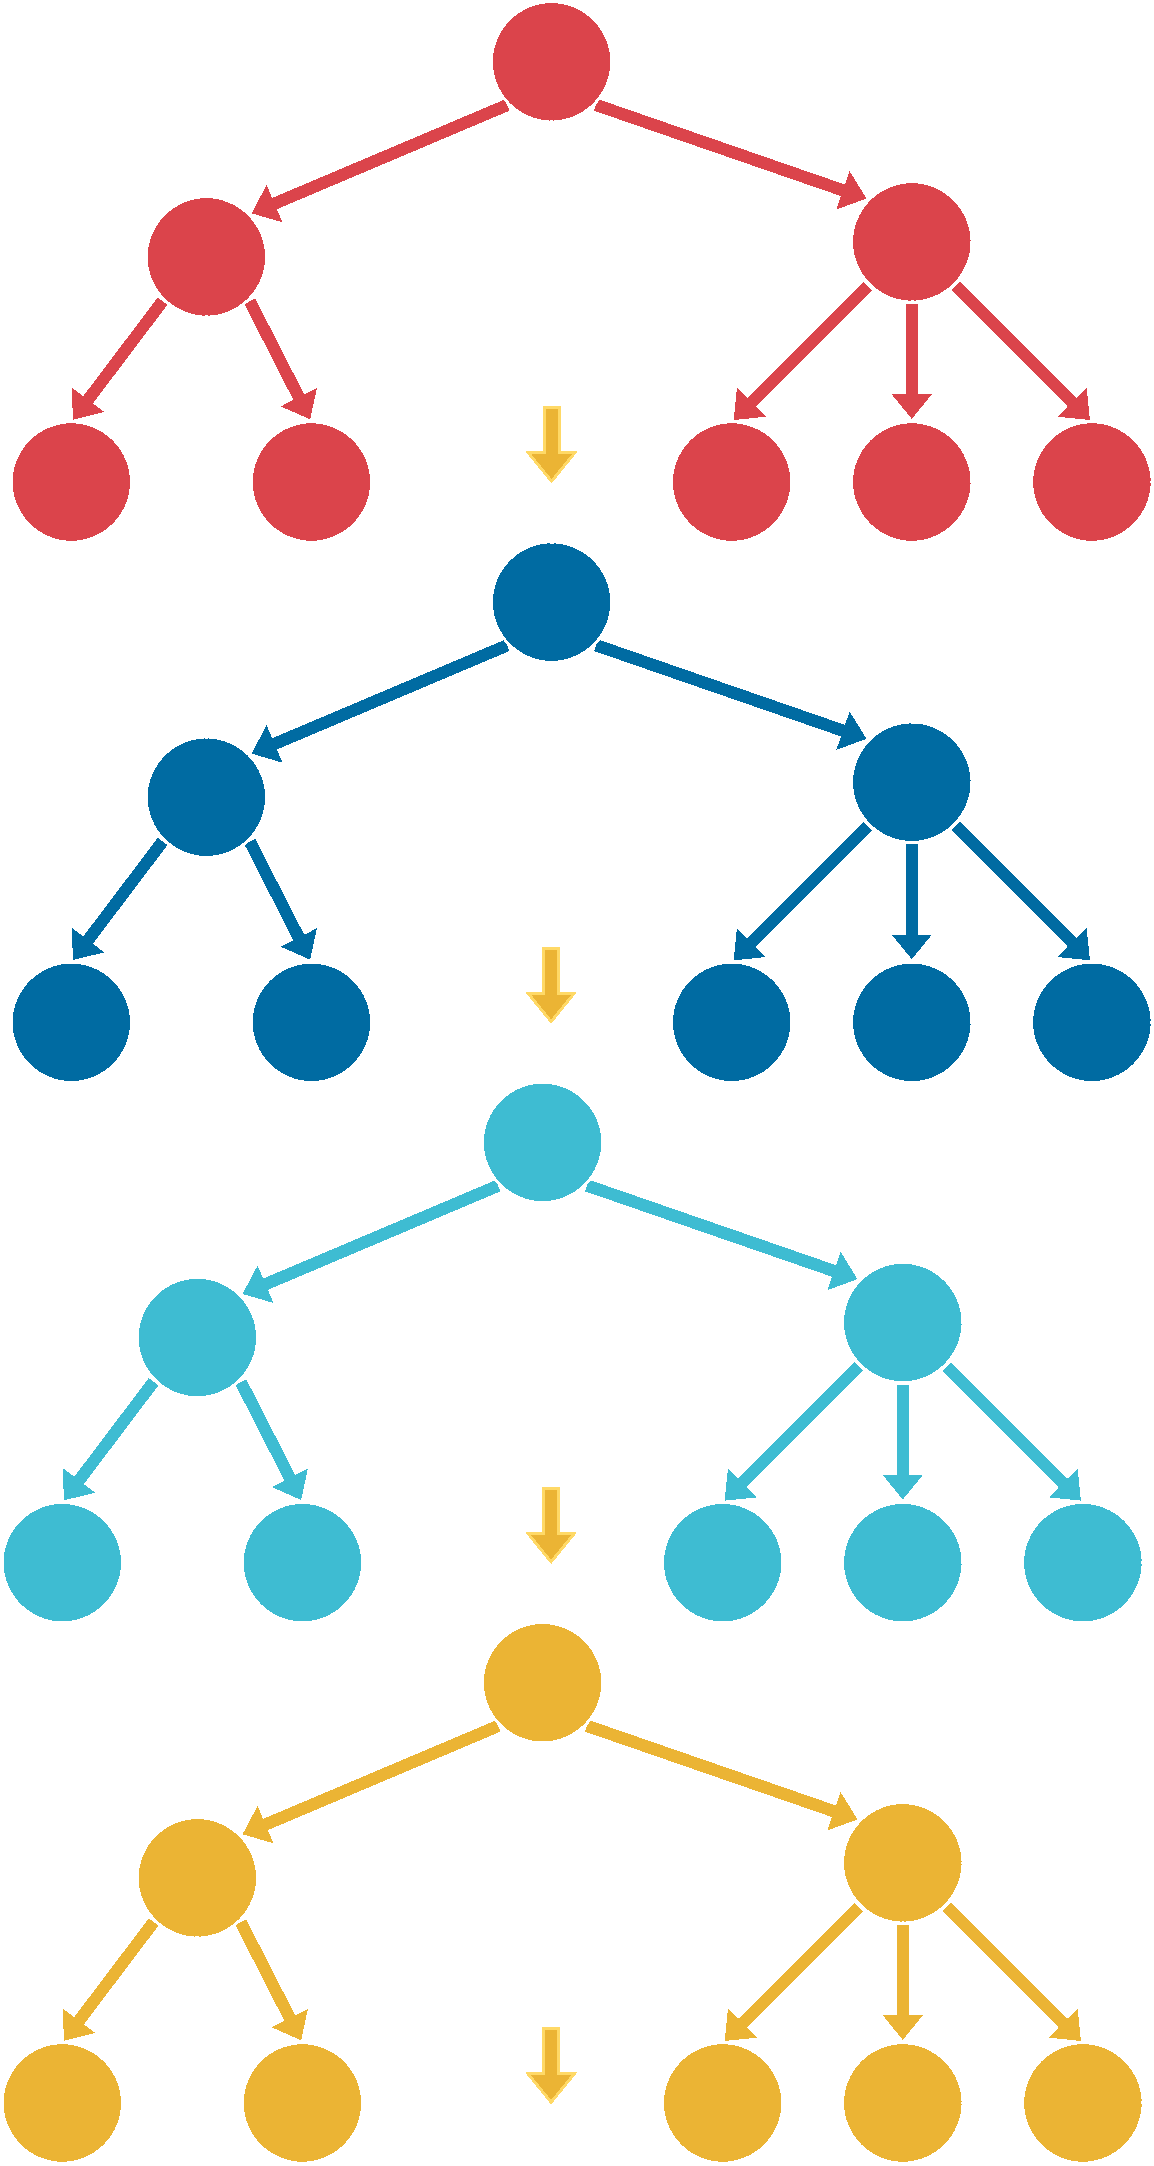
\includegraphics[width=\linewidth, height=\linewidth, keepaspectratio]{images/xgb.drawio.pdf}
        \caption{}
        \label{fig:draw-io-xgboost}
    \end{subfigure}
    \vspace{1em}
    \caption{From Tree Models (a) to Random Forest (b) to Tree Boosting (c)}
    \label{from-decision-tree-to-xgboost}
\end{figure}


\subsubsection{Boosting}

\textcite{schapire-the-strength-of-weak-learners} introduced the first procedure for boosting. He showed that weak learners could improve its model performance when training additional classifiers \parencite{schapire-the-strength-of-weak-learners}. In this context, a weak learner is an algorithm for producing a two-class classifier which outperform random chance. The weak learner algorithm improves on an initial classifier $h_1$ by boosting the model performance, as shown in \autoref{schapire-algo}. \textcite{schapire-the-strength-of-weak-learners} was first able to prove that the boosted classifier $h_B$ outperform the initial $h_1$ in model performance.

\begin{algorithm}[H]
\caption{Schapire Weak Learner Algorithm}
\label{schapire-algo}
\begin{algorithmic}[1]
\Statex \textbf{Input:} Data training set $D$, number of data points $N$.
\State $h_1$ is learned on first $N$ training points in $D$;
\State $h_2$ is learned on a new sample of $N$ point in $D$, where half are misclassified by $h_1$;
\State $h_3$ is learned on $N$ points in $D$, where $h_1$ and $h_2$ disagree
\State $h_B$ is the boosted classifier, where $h_B = \text{Majority Vote}(h_1,h_2,h_3)$
\Statex \textbf{Output:} Boosted classifier $h_B$
\end{algorithmic}
\end{algorithm}

\textcite{freund-boosting-by-majority} expanded the single boosting algorithm with the introduction of boosting by majority, which laid the foundation of the first practical additive boosting algorithm, AdaBoost \parencite{freund-ada-boost}. In AdaBoost, a weak classifier is fitted iteratively to differently weighted versions of the data \parencite{freund-ada-boost}. Data is then reweighted at each iteration, where larger weights are added to misclassified data \parencite{freund-ada-boost}. 

\textcite{ntnu-thesis-why-does-xgboost-win-every-machine-learning-competition} illustrate the additive boosting model, as shown in \autoref{adaboost}. The binary response variable $\Tilde{y}\in\{-1,1\}$ is classified by $c(x)\equiv\text{sign}(f(x))$ where $f(x)\in \Re$. Here, $\Tilde{y}f(x)$ is the margin (steepest ascent). The weak classifiers are shown as $\hat{c}_m(x)\in{\{-1,1\}}$. Classifications in this model are made by by $\hat{c}(x)=\text{sign}(\hat{f}(x))$, where positive/negative values for $\hat{c}(x)$ are correct/false respectively. The final model $\hat{f}(x)$ is result of models $\hat{f}^{(M)}(x)$, where weights $\hat{\theta}_m$ and the weak classifiers $\hat{c}_m(x)$ are iterated over $m$ for $m=1,\dots,M$ \parencite{ntnu-thesis-why-does-xgboost-win-every-machine-learning-competition}. 

\begin{equation}
\label{adaboost}
    \hat{f}(x)\equiv\hat{f}^{(M)}(x)=\sum_{m=1}^{M}\hat{\theta}_m\hat{c}_m(x)
\end{equation}

In \autoref{ensemble-step} \textcite{ntnu-thesis-why-does-xgboost-win-every-machine-learning-competition} show how the current function estimate $f^{(m-1)}$ take the "step" $f_m$ in function space to obtain $f^{(m)}$ for $m=0,\dots,M$. In other words, this shows the update to the tree model at iteration $m$ for each $x\in \mathcal{X}$. Here, function space refer to the mathematical domain where functions (not numerical values) are analysed. The "step" refers to an incremental function in that space. \textcite{ntnu-thesis-why-does-xgboost-win-every-machine-learning-competition} show the resulting estimate of $f$ after $M$ iterations in \autoref{ensemble-bosting}. Note that $f_{m=o}(x)$ represent the initial model. 

\vspace{-1em}
\begin{equation}
\label{ensemble-step}
    f^{(m)}(x)=f^{(m-1)}(x)+f_m(x)
\end{equation}
\begin{equation}
\label{ensemble-bosting}
    f(x)\equiv f^{(M)}(x)=\sum_{m=0}^{M}f_m(x)
\end{equation}

In \autoref{adaptive-basis-function} \textcite{ntnu-thesis-why-does-xgboost-win-every-machine-learning-competition} rewrite the boosting fit ensemble models in \autoref{ensemble-bosting} to adaptive basis function models. Here, we use $f_{m=0}(x)=\theta_0$ and $f_m(x)=\theta_m\phi_m(x)$ for $m=1,\dots,M$. Now, $\theta_m$ are the weights for each basis model $\phi_m(x)$. Boosting uses a base learner $\mathcal{L}_\Phi$, where base models $\phi_1,\dots,\phi_M\in\Phi$ are added to improve current model fit. Here, both the base learner and base models are simple. In other words, they typically have high bias and low variance \parencite{ntnu-thesis-why-does-xgboost-win-every-machine-learning-competition}.

\vspace{-1em}
\begin{equation}
\label{adaptive-basis-function}
    f(x)=\theta_0+\sum_{m=1}^{M}\theta_m\phi_m(x)
\end{equation}

\textcite{ntnu-thesis-why-does-xgboost-win-every-machine-learning-competition} note that most boosting algorithms seek to solve \autoref{boosting-algo-solve}. Here, $\{\hat{\theta}_m,\hat{\phi}_m\}$ represent the pair of weight $\hat{\theta}_m$ and base model $\hat{\phi}_m$ being optimised in iteration $m$. The argument of minimisation $\arg\min$ seek to find values for $\hat{\theta}_m$ and $\hat{\phi}_m$ which minimise the loss function $L$. This is done for each feature vector $x_i$ of data point $i$, where $i=1,\dots,n$. In the loss function $L$, $\theta_m$ is the weight which decide contribution of base model $\phi_m(x)$ to the overall model \parencite{ntnu-thesis-why-does-xgboost-win-every-machine-learning-competition}. 

\vspace{-1em}
\begin{equation}
\label{boosting-algo-solve}
    \{\hat{\theta}_m,\hat{\phi}_m\} = \arg\min_{\{\theta_m,\phi_m\}} \sum_{i=1}^{n} L(y_i,\hat{f}^{(m-1)}(x_i)+\theta_m\phi_m(x_i))
\end{equation}

\subsubsection{Gradient Boosting}

Following tree boosting algorithms producing competitive and highly robust classification models, \textcite{friedman-greedy-function-approximation} introduced Gradient Boosting. This is based on gradient descent in function space. In other words, Gradient Boosting seeks to optimise an algorithm by finding the minimum of a function. It does so by moving opposite to the functions gradient, or steepest ascent. In the next sections we use empirical risk $L(y,f)$ rather than true risk $R(f)$ \parencite{ntnu-thesis-why-does-xgboost-win-every-machine-learning-competition}. 

In \autoref{gradient-algo-3} \textcite{ntnu-thesis-why-does-xgboost-win-every-machine-learning-competition} show the empirical negative gradient $-\hat{g}_m(x_i)$. Here, the empirical gradient $\hat{g}_m(x_i)$ is defined for data points $\{x_i\}_{i=1}^{n}$. The loss function $L(y_i,f(x_i))$ is shown together with its partial derivative. Next, $y_i$ is the true value for the $i$-th data point $x$ where $x\in\mathcal{X}$. The subscript show the model prediction $f(x_i)$ at data point $x_i$, together with the estimate of the previous iteration $\hat{f}^{(m-1)}(x)$. The subscript indicate that the partial derivative are evaluated from the previous iteration $m-1$ \parencite{ntnu-thesis-why-does-xgboost-win-every-machine-learning-competition}. 

\vspace{-1em}
\begin{equation}
\label{gradient-algo-3}
    -\hat{g}_{m}(x_i) = -\left[\frac{\partial L(y_i, f(x_i))}{\partial f(x_i)} \right]_{f(x)=\hat{f}^{(m-1)}(x)}
\end{equation}

In \autoref{newton-algo-4}, we generalise the empirical gradient $\hat{g}_m(x_i)$ for other data points in $\mathcal{X}$ while preventing over-fitting \parencite{ntnu-thesis-why-does-xgboost-win-every-machine-learning-competition}. This can be done by learning an approximate negative gradient $\{\phi_m(x_i)\}_{i=1}^{n}$, which is correlated to the negative empirical gradient $\{-\hat{g}_m(x_i)\}_{i=1}^{n}$, and constrained by the set of basis functions $\Phi$. Here, the basis functions $\phi_m\in\Phi$ is learnt from the data at iteration $m$. The argument of minimisation $\arg\min$ search for basis functions $\phi\in\Phi$ and coefficient $\beta$, iterated over $i=1,\dots,n$. It does so, trying to minimise the squared sum of differences between the negative gradient $-\hat{g}_m(x_i)$ and scaled basis function $\beta\phi(x_i)$. The base function $\phi_m$ is thereby learned using squared loss error. In short, this sequence is used to learn a direction for gradient descent constrained by the set of basis functions $\Phi$ \parencite{ntnu-thesis-why-does-xgboost-win-every-machine-learning-competition}.  

\begin{equation}
\label{gradient-algo-4}
\hat{\phi}_m=\arg\min_{\phi\in\Phi,\beta}\sum_{i=1}^{n}\left[ (-\hat{g}_{m}(x_i)) - \beta\phi(x_i) \right]^2
\end{equation}

In \autoref{gradient-algo-5} we go further than "step" direction, and illustrate "step" length $\rho_m$ in the function space \parencite{ntnu-thesis-why-does-xgboost-win-every-machine-learning-competition}. Here, the argument of minimisation $\arg\min$ find values of $\rho_m$ for iteration $m$, which minimise the loss function $L$. As before, $\hat{f}^{(m-1)}(x_i)$ is the model prediction, and $\hat{\phi}_m(x_i)$ is the basis function, both for data point $x_i$ where $i=1,\dots,n$.  

\begin{equation}
\label{gradient-algo-5}
    \hat{\rho}_m = \arg\min_{\rho} \sum_{i=1}^{n}L(y_i,\hat{f}^{(m-1)}(x_i)+\rho\hat{\phi}_m(x_i))
\end{equation}

Continuing on "step" length $\rho_m$, \textcite{friedman-greedy-function-approximation} introduced the shrinkage term $\eta$ where $0<\eta\leq1$. This term is multiplied with "step" length $\rho_m$ at each iteration $m$. \textcite{ntnu-thesis-why-does-xgboost-win-every-machine-learning-competition} illustrate this in \autoref{newton-algo-6}. This concludes the "step" $\hat{f}_m(x)$ at iteration $m$, which is found using the basis function $\hat{\phi}_m(x)$, "step" length $\hat{\rho}_m$, and shrinkage term $\eta$ \parencite{ntnu-thesis-why-does-xgboost-win-every-machine-learning-competition}.

\begin{equation}
\label{gradient-algo-6}
    \hat{f}_m(x)=\eta\hat{\rho}_m\hat{\phi}_m(x)
\end{equation}

\subsubsection{Hessian Boosting}

In the context of introducing Gradient Boosting, Hessian Boosting has been discussed by \textcite{friedman-greedy-function-approximation}. Hessian Boosting can also be referred to as Newton Boosting, or Second-Order Gradient Boosting as done by \textcite{ntnu-thesis-why-does-xgboost-win-every-machine-learning-competition}. In short, the move from Gradient to Hessian Boosting includes using not only first-order (Gradient), but also second-order (Hessian) methods when optimising boosting algorithms. 

In \autoref{newton-algo-4} we illustrate the empirical Hessian $\hat{h}_{m}(x_i)$ \parencite{ntnu-thesis-why-does-xgboost-win-every-machine-learning-competition}. The intuition for the loss function $L(y_i,f(x_i)$, its partial derivative, and the subscript with model prediction $f(x_i)$ and estimate of previous iteration $\hat{f}^{(m-1)}(x)$ follow the intuition of \autoref{gradient-algo-3} \parencite{ntnu-thesis-why-does-xgboost-win-every-machine-learning-competition}. 

\begin{equation}
\label{newton-algo-4}
    \hat{h}_{m}(x_i)=\left[\frac{\partial^{2} L(y_i, f(x_i))}{\partial f(x_i)^{2}} \right]_{f(x)=\hat{f}^{(m-1)}(x)}
\end{equation}

In \autoref{newton-algo-5} we show the Newton "step" in function space $\hat{\phi}_m$ at iteration $m$ \parencite{ntnu-thesis-why-does-xgboost-win-every-machine-learning-competition}. This is found using the argument of minimisation $\arg\min$ of the sum squared difference between a scaled version of the empirical negative gradient $-\hat{g}_m(x_i)/\hat{h}_m(x_i)$ and the base function $\phi(x_i)$. The optimised term is also multiplied by the factored Hessian gradient $1/2\cdot\hat{h}_m(x_i)$ \parencite{ntnu-thesis-why-does-xgboost-win-every-machine-learning-competition}. 

\begin{equation}
\label{newton-algo-5}
    \hat{\phi}_m = \arg\min_{\phi\in\Phi} \sum_{i=1}^{n} \frac{1}{2} \hat{h}_m(x_i) \left[ (-\frac{\hat{g}_m(x_i)}{\hat{h}_m(x_i)}) - \phi(x_i) \right] ^2
\end{equation}

To sum, the "step" $\hat{f}_m(x)$ taken in function space is illustrated in \autoref{newton-algo-6} \parencite{ntnu-thesis-why-does-xgboost-win-every-machine-learning-competition}. Note the shrinkage term $\eta$ where $0<\eta\leq1$, and the Newton "step" $\hat{\phi}_m(x)$. 

\begin{equation}
\label{newton-algo-6}
    \hat{f}_m(x) = \eta\hat{\phi}_m(x)
\end{equation}

\subsubsection{The Hessian Boosting Algorithm}

Iterating the steps in \autoref{gradient-algo-3} and from \autoref{newton-algo-4} to \autoref{newton-algo-6} give the Hessian Boosting algorithm, as shown in \autoref{extreme-gradient-algo} \parencite{ntnu-thesis-why-does-xgboost-win-every-machine-learning-competition}. One can initialise the Hessian Boosting algorithm using a constant $f_0(x)$, as shown in \autoref{newton-algo-1} where the estimated initial $\hat{\theta}_0$ is shown in \autoref{newton-algo-theta-1} \parencite{ntnu-thesis-why-does-xgboost-win-every-machine-learning-competition}.  

\begin{equation}
\label{newton-algo-1}
    f_0(x)=\theta_0
\end{equation}
\begin{equation}
\label{newton-algo-theta-1}
    \hat{\theta}_0 = \arg\min_{\theta}\sum_{i=1}^{n}L(y_i,\theta)
\end{equation}

The Hessian Boosting algorithm give the resulting model shown in \autoref{newton-algo-output}. This can be viewed as an adaptive basis function model $\hat{f}_m(x)$, illustrated in \autoref{newton-algo-7} where $\hat{\theta}_m=\eta$ for $m=1,\dots,M$ \parencite{ntnu-thesis-why-does-xgboost-win-every-machine-learning-competition}. 

\begin{equation}
\label{newton-algo-output}
    \hat{f}(x) \equiv \hat{f}^{(M)}(x) = \sum_{m=0}^M\hat{f}_m(x)
\end{equation}
\begin{equation}
\label{newton-algo-7}
    \hat{f}^{(m)}(x)=\hat{\theta}_{m}\hat{\phi}_m
\end{equation}

\begin{algorithm}[H]
\caption{Hessian Boosting algorithm}
\label{extreme-gradient-algo}
\begin{algorithmic}
\Statex \textbf{Input:} Data set \(D\), loss function \(L\), base learner \(\mathcal{L}_{\Phi}\), iterations $M$, and shrinkage \(\eta\).
\vspace{1em}
\Statex 1: Initialise \(\hat{f}^{(0)}(x) = \hat{f}_0(x) = \hat{\theta}_0 = \arg\min_{\theta} \sum_{i=1}^n L(y_i, \theta)\);
\vspace{1em}
\For{\(m = 1,2,\ldots,M\)}
\vspace{1em}
    \Statex \quad 2: $\hat{g}_{m}(x_i) = \left[\frac{\partial L(y_i, f(x_i))}{\partial f(x_i)} \right]_{f(x)=\hat{f}^{(m-1)}(x)}$;
    \vspace{1em}
    \Statex \quad 3: $\hat{h}_{m}(x_i)=\left[\frac{\partial^{2} L(y_i, f(x_i))}{\partial f(x_i)^{2}} \right]_{f(x)=\hat{f}^{(m-1)}(x)}$;
    \vspace{1em}
    \Statex \quad 4: \(\hat{\phi}_m = \arg\min_{\phi \in \Phi} \sum_{i=1}^n \frac{1}{2} \hat{h}_m(x_i) \left[ (- \frac{\hat{g}_m(x_i)}{\hat{h}_m(x_i)}) - \phi(x_i) \right]^2 \);
    \vspace{1em}
    \Statex \quad 5: \(\hat{f}_m(x) = \eta \hat{\phi}_m(x)\);
    \vspace{1em}
    \Statex \quad 6: \(\hat{f}^{(m)}(x) = \hat{f}^{(m-1)}(x) + \hat{f}_m(x)\);
\vspace{1em}
\EndFor
\vspace{1em}
\Statex \textbf{Output:} \(\hat{f}(x) \equiv \hat{f}^{(M)}(x) = \sum_{m=0}^M \hat{f}_m(x)\)
\end{algorithmic}
\end{algorithm}




% Table created by stargazer v.5.2.3 by Marek Hlavac, Social Policy Institute. E-mail: marek.hlavac at gmail.com
% Date and time: Mon, Dec 11, 2023 - 11:20:49
\begin{table}[H] 
\centering 
  \caption{Fama-French Regression for Long-Short Trading Portfolios} 
  \subcaption*{Table \thetable.1:}
  \label{table:FAMA-FRENCH-LONG-SHORT-TRADING-FINAL} 
\begin{tabularx}{\textwidth}{XXXXXXXXXXl} 
\\[-1.8ex]\hline 
\hline \\[-1.8ex] 
 & \multicolumn{10}{c}{\textit{Dependent variable:}} \\ 
\cline{2-11} 
\\[-1.8ex] 
 & \multicolumn{3}{c}{GLM} & \multicolumn{3}{c}{XGBB} & \multicolumn{3}{c}{XGBC} & \\
 \cline{2-11}
 \\[-1.8ex] 
 & 30 & 60 & 100 & 30 & 60 & 100 & 30 & 60 & 100 & OSEBX \\ 
 \cline{2-11} \\
 SMB & 0.002 & 0.055 & 0.200 & 0.004 & 0.070 & 0.222$^{**}$ & 0.029 & 0.066 & 0.181$^{**}$ & 0.087 \\ 
  & (0.104) & (0.135) & (0.145) & (0.097) & (0.109) & (0.105) & (0.088) & (0.092) & (0.087) & (0.086) \\ 
  & & & & & & & & & & \\ 
 HML & 0.108 & 0.029 & $-$0.011 & 0.167$^{**}$ & 0.164$^{**}$ & 0.062 & 0.123$^{*}$ & 0.125$^{*}$ & 0.061 & 0.140$^{**}$ \\ 
  & (0.075) & (0.097) & (0.105) & (0.070) & (0.079) & (0.076) & (0.063) & (0.066) & (0.063) & (0.062) \\ 
  & & & & & & & & & & \\ 
 UMD & $-$0.178$^{**}$ & $-$0.082 & $-$0.043 & $-$0.189$^{***}$ & $-$0.063 & $-$0.017 & $-$0.200$^{***}$ & $-$0.158$^{**}$ & $-$0.082 & $-$0.218$^{***}$ \\ 
  & (0.074) & (0.097) & (0.104) & (0.069) & (0.078) & (0.075) & (0.063) & (0.066) & (0.063) & (0.061) \\ 
  & & & & & & & & & & \\ 
 $\alpha$ & \cellcolor{lightlightgreen}0.014$^{***}$ & 0.011$^{*}$ & 0.010 & \cellcolor{lightlightgreen}0.013$^{***}$ & 0.007 & 0.002 & \cellcolor{lightlightgreen}0.013$^{***}$ & 0.009$^{**}$ & 0.005 & 0.012$^{***}$ \\ 
  & (0.005) & (0.006) & (0.006) & (0.004) & (0.005) & (0.005) & (0.004) & (0.004) & (0.004) & (0.004) \\ 
  & & & & & & & & & & \\ 
\hline \\[-1.8ex] 
Obs & 155 & 155 & 155 & 155 & 155 & 155 & 155 & 155 & 155 & 155 \\ 
R$^{2}$ & 0.043 & 0.006 & 0.015 & 0.069 & 0.030 & 0.031 & 0.075 & 0.052 & 0.041 & 0.097 \\ 
R$^{2}$_{adj} & 0.024 & $-$0.014 & $-$0.005 & 0.051 & 0.011 & 0.012 & 0.056 & 0.034 & 0.022 & 0.079 \\ 
RSE & 0.051 & 0.066 & 0.071 & 0.048 & 0.053 & 0.052 & 0.043 & 0.045 & 0.043 & 0.042 \\ 
(df=151) & & & & & & & & & & \\
F_{score} & 2.280$^{*}$ & 0.307 & 0.753 & 3.740$^{**}$ & 1.572 & 1.614 & 4.064$^{***}$ & 2.788$^{**}$ & 2.157$^{*}$ & 5.417$^{***}$ \\ 
(df=3;151) & & & & & & & & & & \\
\hline 
\hline \\[-1.8ex] 
\textit{Note:}  & \multicolumn{10}{r}{$^{*}$p$<$0.1; $^{**}$p$<$0.05; $^{***}$p$<$0.01} \\ 
\end{tabularx} 
\end{table} 

In addition to the intercept ($\alpha$), we also observe some significant relation

% LONG ONLY FAMA FRENCH RESULTS TRADING
% Date and time: Mon, Dec 11, 2023 - 11:25:06
\begin{table}[H] 
  \caption{Fama-French Regression for Long-Only Trading Portfolios} 
  \subcaption*{Table \thetable.1:}
  \label{table:FAMA-FRENCH-LONG-ONLY-TRADING-FINAL} 
\begin{tabularx}{\textwidth}{XXXXXXXXXXl} 
\\[-1.8ex]\hline 
\hline \\[-1.8ex] 
 & \multicolumn{10}{c}{\textit{Dependent variable:}} \\ 
\cline{2-11} 
\\[-1.8ex] 
& \multicolumn{3}{c}{GLM L} & \multicolumn{3}{c}{XGBB L} & \multicolumn{3}{c}{XGBC L} & \\
\cline{2-11}
\\[-1.8ex] 
& 30 & 60 & 100 & 30 & 60 & 100 & 30 & 60 & 100 & OSEBX \\ 
\cline{2-11} \\
 SMB & 0.103 & 0.145 & 0.300$^{**}$ & 0.118 & 0.192$^{*}$ & 0.350$^{**}$ & 0.110 & 0.172 & 0.237$^{**}$ & 0.087 \\ 
  & (0.093) & (0.115) & (0.121) & (0.097) & (0.106) & (0.138) & (0.090) & (0.104) & (0.119) & (0.086) \\ 
  & & & & & & & & & & \\ 
 HML & 0.166$^{**}$ & 0.126 & 0.077 & 0.170$^{**}$ & 0.162$^{**}$ & 0.141 & 0.132$^{**}$ & 0.109 & 0.105 & 0.140$^{**}$ \\ 
  & (0.067) & (0.083) & (0.088) & (0.070) & (0.076) & (0.100) & (0.065) & (0.075) & (0.086) & (0.062) \\ 
  & & & & & & & & & & \\ 
 UMD & $-$0.208$^{***}$ & $-$0.184$^{**}$ & $-$0.160$^{*}$ & $-$0.222$^{***}$ & $-$0.175$^{**}$ & $-$0.137 & $-$0.223$^{***}$ & $-$0.225$^{***}$ & $-$0.155$^{*}$ & $-$0.218$^{***}$  \\ 
  & (0.066) & (0.083) & (0.087) & (0.070) & (0.076) & (0.099) & (0.065) & (0.075) & (0.085) & (0.061) \\ 
  & & & & & & & & & & \\ 
 $\alpha$ & 0.012$^{***}$ & 0.008 & 0.003 & \cellcolor{lightlightgreen}0.013$^{***}$ & 0.010$^{**}$ & 0.008 & \cellcolor{lightlightgreen}0.013$^{***}$ & 0.010$^{**}$ & 0.009$^{*}$ & 0.012$^{***}$ \\ 
  & (0.004) & (0.005) & (0.005) & (0.004) & (0.005) & (0.006) & (0.004) & (0.005) & (0.005) & (0.004) \\ 
  & & & & & & & & & & \\ 
\hline \\[-1.8ex] 
Obs & 155 & 155 & 155 & 155 & 155 & 155 & 155 & 155 & 155 & 155 \\ 
R$^{2}$ & 0.088 & 0.048 & 0.062 & 0.090 & 0.069 & 0.058 & 0.093 & 0.078 & 0.050 & 0.097 \\ 
R$^{2}$_{adj} & 0.070 & 0.030 & 0.043 & 0.072 & 0.050 & 0.040 & 0.075 & 0.059 & 0.031 & 0.079 \\ 
RSE & 0.046 & 0.057 & 0.060 & 0.048 & 0.052 & 0.068 & 0.044 & 0.051 & 0.059 & 0.042 \\ 
(df=151) & & & & & & & & & & \\
F_{score} & 4.882$^{***}$ & 2.563$^{*}$ & 3.324$^{**}$ & 4.960$^{***}$ & 3.720$^{**}$ & 3.126$^{**}$ & 5.143$^{***}$ & 4.239$^{***}$ & 2.660$^{*}$ & 5.417$^{***}$ \\ 
(df=3;151) & & & & & & & & & & \\
\hline 
\hline \\[-1.8ex] 
\textit{Note:}  & \multicolumn{10}{r}{$^{*}$p$<$0.1; $^{**}$p$<$0.05; $^{***}$p$<$0.01} \\ 
\end{tabularx} 
\end{table}







% Long-short enhanced
\begin{table}[H]  
  \caption{Fama-French Regression for Long-Short Enhanced Index Portfolios} 
  \subcaption*{Table \thetable.1:}
  \label{table:FAMA-FRENCH-LONG-SHORT-ENHANCED-FINAL} 
\begin{tabularx}{\textwidth}{XXXXXXXXXXl} 
\\[-2ex]\hline 
\hline \\[-2ex] 
 & \multicolumn{10}{c}{\textit{Dependent variable:}} \\ 
\cline{2-11} 
\\[-2ex] 
 & \multicolumn{3}{c}{GLM} & \multicolumn{3}{c}{XGBB} & \multicolumn{3}{c}{XGBC} & \\
 \cline{2-11}
 \\[-2ex] 
 & 30 & 60 & 100 & 30 & 60 & 100 & 30 & 60 & 100 & OSEBX \\ 
 \cline{2-11} \\
 SMB & 0.077 & 0.085 & 0.094 & 0.074 & 0.084 & 0.095 & 0.073 & 0.084 & 0.095 & 0.087 \\ 
  & (0.085) & (0.085) & (0.085) & (0.085) & (0.084) & (0.082) & (0.085) & (0.084) & (0.082) & (0.086) \\ 
  %& & & & & & & & & & \\ 
 HML & 0.136$^{**}$ & 0.132$^{**}$ & 0.131$^{**}$ & 0.146$^{**}$ & 0.143$^{**}$ & 0.137$^{**}$ & 0.136$^{**}$ & 0.139$^{**}$ & 0.134$^{**}$ & 0.140$^{**}$ \\ 
  & (0.061) & (0.062) & (0.061) & (0.062) & (0.060) & (0.059) & (0.061) & (0.060) & (0.059) & (0.062) \\ 
  %& & & & & & & & & & \\ 
 UMD & $-$0.212$^{***}$ & $-$0.208$^{***}$ & $-$0.205$^{***}$ & $-$0.213$^{***}$ & $-$0.202$^{***}$ & $-$0.204$^{***}$ & $-$0.214$^{***}$ & $-$0.210$^{***}$ & $-$0.207$^{***}$ & $-$0.218$^{***}$ \\ 
  & (0.061) & (0.061) & (0.061) & (0.061) & (0.060) & (0.059) & (0.061) & (0.060) & (0.059) & (0.061) \\ 
  %& & & & & & & & & & \\ 
 $\alpha$ & 0.012$^{***}$ & 0.012$^{***}$ & 0.012$^{***}$ & 0.012$^{***}$ & 0.011$^{***}$ & 0.011$^{***}$ & 0.012$^{***}$ & 0.011$^{***}$ & 0.011$^{***}$ & 0.012$^{***}$ \\ 
  & (0.004) & (0.004) & (0.004) & (0.004) & (0.004) & (0.004) & (0.004) & (0.004) & (0.004) & (0.004) \\ 
  %& & & & & & & & & & \\ 
\hline \\[-2ex] 
Obs & 155 & 155 & 155 & 155 & 155 & 155 & 155 & 155 & 155 & 155 \\ 
R$^{2}$ & 0.093 & 0.090 & 0.091 & 0.096 & 0.093 & 0.097 & 0.095 & 0.096 & 0.098 & 0.097 \\ 
R$^{2}$_{adj} & 0.075 & 0.072 & 0.073 & 0.078 & 0.075 & 0.079 & 0.077 & 0.078 & 0.080 & 0.079 \\ 
RES & 0.042 & 0.042 & 0.042 & 0.042 & 0.041 & 0.040 & 0.042 & 0.041 & 0.040 & 0.042 \\ 
(df=151) & & & & & & & & & & \\
F_{score} & 5.150$^{***}$ & 4.974$^{***}$ & 5.015$^{***}$ & 5.327$^{***}$ & 5.140$^{***}$ & 5.382$^{***}$ & 5.279$^{***}$ & 5.343$^{***}$ & 5.460$^{***}$ & 5.417$^{***}$ \\
(df=3;151) & & & & & & & & & & \\
\hline 
\hline \\[-2ex] 
\textit{Note:}  & \multicolumn{10}{r}{$^{*}$p$<$0.1; $^{**}$p$<$0.05; $^{***}$p$<$0.01} \\ 
\end{tabularx} 
\end{table} 

In the Fama-French regression models, we ob

% Long-only enhanced
\begin{table}[H] 
  \caption{Fama-French Regression for Long-Only Enhanced Index Portfolios} 
  \subcaption*{Table \thetable.1:}
  \label{table:FAMA-FRENCH-LONG-ONLY-ENHANCED-FINAL} 
\begin{tabularx}{\textwidth}{XXXXXXXXXXl} 
\\[-1.8ex]\hline 
\hline \\[-1.8ex] 
 & \multicolumn{10}{c}{\textit{Dependent variable:}} \\ 
\cline{2-11} 
\\[-1.8ex] 
& \multicolumn{3}{c}{GLM L} & \multicolumn{3}{c}{XGBB L} & \multicolumn{3}{c}{XGBC L} & \\
\cline{2-11}
\\[-1.8ex] 
& 30 & 60 & 100 & 30 & 60 & 100 & 30 & 60 & 100 & OSEBX \\ 
\cline{2-11} \\
 SMB & 0.091 & 0.092 & 0.108 & 0.094 & 0.100 & 0.110 & 0.093 & 0.101 & 0.104 & 0.087 \\ 
  & (0.086) & (0.086) & (0.085) & (0.086) & (0.086) & (0.084) & (0.085) & (0.086) & (0.085) & (0.086) \\ 
  & & & & & & & & & & \\ 
 HML & 0.146$^{**}$ & 0.139$^{**}$ & 0.135$^{**}$ & 0.146$^{**}$ & 0.143$^{**}$ & 0.140$^{**}$ & 0.139$^{**}$ & 0.135$^{**}$ & 0.135$^{**}$ & 0.140$^{**}$ \\ 
  & (0.062) & (0.062) & (0.061) & (0.062) & (0.062) & (0.061) & (0.061) & (0.062) & (0.061) & (0.062) \\ 
  & & & & & & & & & & \\ 
 UMD & $-$0.216$^{***}$ & $-$0.214$^{***}$ & $-$0.211$^{***}$ & $-$0.219$^{***}$ & $-$0.212$^{***}$ & $-$0.212$^{***}$ & $-$0.220$^{***}$ & $-$0.219$^{***}$ & $-$0.211$^{***}$ & $-$0.218$^{***}$ \\ 
  & (0.062) & (0.062) & (0.061) & (0.061) & (0.061) & (0.060) & (0.061) & (0.062) & (0.061) & (0.061) \\ 
  & & & & & & & & & & \\ 
 $\alpha$ & 0.012$^{***}$ & 0.011$^{***}$ & 0.011$^{***}$ & 0.012$^{***}$ & 0.011$^{***}$ & 0.011$^{***}$ & 0.012$^{***}$ & 0.012$^{***}$ & 0.011$^{***}$ & 0.012$^{***}$ \\ 
  & (0.004) & (0.004) & (0.004) & (0.004) & (0.004) & (0.004) & (0.004) & (0.004) & (0.004) & (0.004) \\ 
  & & & & & & & & & & \\ 
\hline \\[-1.8ex] 
Obs & 155 & 155 & 155 & 155 & 155 & 155 & 155 & 155 & 155 & 155 \\ 
R$^{2}$ & 0.098 & 0.094 & 0.097 & 0.100 & 0.096 & 0.100 & 0.100 & 0.097 & 0.097 & 0.097 \\ 
R$^{2}$_{adj} & 0.080 & 0.076 & 0.079 & 0.082 & 0.078 & 0.082 & 0.082 & 0.079 & 0.079 & 0.079 \\ 
RES & 0.042 & 0.042 & 0.042 & 0.042 & 0.042 & 0.041 & 0.042 & 0.042 & 0.042 & 0.042 \\ 
(df=151) & & & & & & & & & & \\
F_{stat} & 5.452$^{***}$ & 5.241$^{***}$ & 5.377$^{***}$ & 5.595$^{***}$ & 5.361$^{***}$ & 5.609$^{***}$ & 5.579$^{***}$ & 5.433$^{***}$ & 5.396$^{***}$ & 5.417$^{***}$ \\
(df=3;151) & & & & & & & & & & \\
\hline 
\hline \\[-1.8ex] 
\textit{Note:}  & \multicolumn{10}{r}{$^{*}$p$<$0.1; $^{**}$p$<$0.05; $^{***}$p$<$0.01} \\ 
\end{tabularx} 
\end{table} 



We used machine learning to exploit the \textit{index effect}, which is a financial phenomena where companies announced to be included in a benchmark index tends to experience increased share price in the time before the company is included in the index. To exploit the Index Effect we used machine learning to predict if companies will be included on the Oslo Stock Exchange Benchmark Index (OSEBX), and simulated portfolios where we bought the companies predicted to enter the index, and selling companies predicted to exit. Furthermore, we investigated if this investing strategy would be exploitable in Enhanced Index Portfolio Management.

Our findings indicate that eXtreme Gradient Boosting with a custom post-processing step for risk adjustment performs best in terms of predicting additions and deletions to OSEBX, which also yielded the best-performing portfolios in terms of risk-adjusted Alpha. On average, the long-only eXtreme Gradient Boosting model, with a holding horizon of 30 days before the effective date of the rebalancing, gave an average monthly return of 1.44\% from 2010 to 2023, beating OSEBX by 2.4\% per year.

Surprisingly enough, our finding support that there might exist a market-weakness, as the underlying value of a company should not change based on whether or not the company is included on OSEBX. One possible explanation to this weakness might be that passive index-funds are, to an extend, forced to hold the companies included on the index, as the fund manager has promised to his or her investors.




% updated 14.12 long-short
\begin{table}[H] \centering 
  \caption{Fama-French 3 Factor Model Regression for Long-Short Enhanced Index Portfolios} 
  \subcaption*{}
  \label{} 
\begin{tabularx}{\textwidth}{XXXXXXXXXXl} 
\\[-1.8ex]\hline 
\hline \\[-1.8ex] 
 & \multicolumn{10}{c}{\textit{Dependent variable:}} \\ 
\cline{2-11} 
\\[-1.8ex] 
 & \multicolumn{3}{c}{GLM} & \multicolumn{3}{c}{XGBB} & \multicolumn{3}{c}{XGBC} & \\
 \cline{2-10}
 \\[-1.8ex] 
 & 30 & 60 & 100 & 30 & 60 & 100 & 30 & 60 & 100 & OSEBX \\ 
 \cline{2-10} \\
 MR & 1.020$^{***}$ & 0.986$^{***}$ & 0.992$^{***}$ & 1.011$^{***}$ & 0.975$^{***}$ & 0.959$^{***}$ & 1.002$^{***}$ & 0.977$^{***}$ & 0.942$^{***}$ & 1.022$^{***}$ \\ 
  & (0.017) & (0.020) & (0.020) & (0.018) & (0.019) & (0.018) & (0.019) & (0.019) & (0.017) & (0.017) \\ 
  & & & & & & & & & & \\ 
 SMB & $-$0.044$^{**}$ & $-$0.046$^{**}$ & $-$0.047$^{**}$ & $-$0.054$^{***}$ & $-$0.047$^{**}$ & $-$0.027 & $-$0.064$^{***}$ & $-$0.046$^{**}$ & $-$0.027 & $-$0.042$^{**}$ \\ 
  & (0.017) & (0.020) & (0.020) & (0.018) & (0.019) & (0.018) & (0.019) & (0.019) & (0.017) & (0.017) \\ 
  & & & & & & & & & & \\ 
 HML & $-$0.016 & $-$0.029$^{*}$ & $-$0.030$^{**}$ & $-$0.006 & $-$0.005 & $-$0.008 & $-$0.013 & $-$0.007 & $-$0.010 & $-$0.016 \\ 
  & (0.013) & (0.015) & (0.014) & (0.013) & (0.014) & (0.013) & (0.014) & (0.014) & (0.013) & (0.013) \\ 
  & & & & & & & & & & \\ 
 $\alpha$_{FF3} & 0.001 & 0.001 & 0.001 & 0.001 & 0.001 & 0.0004 & 0.001$^{*}$ & 0.001 & 0.001 & 0.001 \\ 
  & (0.001) & (0.001) & (0.001) & (0.001) & (0.001) & (0.001) & (0.001) & (0.001) & (0.001) & (0.001) \\ 
  & & & & & & & & & & \\ 
\hline \\[-1.8ex] 
Obs & 148 & 148 & 148 & 148 & 148 & 148 & 148 & 148 & 148 & 148 \\ 
R$^{2}$ & 0.962 & 0.944 & 0.948 & 0.957 & 0.950 & 0.954 & 0.951 & 0.950 & 0.955 & 0.962 \\ 
R$^{2}$_{adj} & 0.961 & 0.943 & 0.947 & 0.956 & 0.949 & 0.953 & 0.950 & 0.949 & 0.954 & 0.961 \\ 
RES & 0.008 & 0.010 & 0.010 & 0.009 & 0.009 & 0.009 & 0.009 & 0.009 & 0.008 & 0.008 \\ 
(df=144) & & & & & & & & & & \\
F_{stat} & 1,212.010$^{***}$ & 813.128$^{***}$ & 870.578$^{***}$ & 1,056.669$^{***}$ & 906.179$^{***}$ & 988.336$^{***}$ & 937.952$^{***}$ & 913.462$^{***}$ & 1,026.743$^{***}$ & 1,223.127$^{***}$ \\ 
(df=3;144) & & & & & & & & & & \\
\hline 
\hline \\[-1.8ex] 
\textit{Note:}  & \multicolumn{10}{r}{$^{*}$p$<$0.1; $^{**}$p$<$0.05; $^{***}$p$<$0.01} \\ 
\end{tabularx} 
\end{table} 



% updated fama french 14.12.2023 long only
\begin{table}[H] \centering 
  \caption{Fama-French 3 Factor Model Regression for Long-Only Enhanced Index Portfolios} 
  \subcaption*{}
  \label{} 
\begin{tabularx}{\textwidth}{XXXXXXXXXXl} 
\\[-1.8ex]\hline 
\hline \\[-1.8ex] 
 & \multicolumn{10}{c}{\textit{Dependent variable:}} \\ 
\cline{2-11} 
\\[-1.8ex] 
 & \multicolumn{3}{c}{GLM} & \multicolumn{3}{c}{XGBB} & \multicolumn{3}{c}{XGBC} & \\
 \cline{2-10}
 \\[-1.8ex] 
 & 30 & 60 & 100 & 30 & 60 & 100 & 30 & 60 & 100 & OSEBX \\ 
 \cline{2-10} \\ 
 MR & 1.015$^{***}$ & 1.026$^{***}$ & 1.025$^{***}$ & 1.025$^{***}$ & 1.010$^{***}$ & 1.000$^{***}$ & 1.020$^{***}$ & 1.015$^{***}$ & 0.995$^{***}$ & 1.022$^{***}$ \\ 
  & (0.022) & (0.021) & (0.019) & (0.017) & (0.019) & (0.022) & (0.018) & (0.020) & (0.018) & (0.017) \\ 
  & & & & & & & & & & \\ 
 SMB & $-$0.052$^{**}$ & $-$0.031 & $-$0.026 & $-$0.032$^{*}$ & $-$0.028 & $-$0.005 & $-$0.035$^{*}$ & $-$0.030 & $-$0.019 & $-$0.042$^{**}$ \\ 
  & (0.022) & (0.021) & (0.019) & (0.017) & (0.019) & (0.022) & (0.018) & (0.020) & (0.018) & (0.017) \\ 
  & & & & & & & & & & \\ 
 HML & $-$0.010 & $-$0.021 & $-$0.021 & $-$0.003 & $-$0.013 & $-$0.009 & $-$0.010 & $-$0.016 & $-$0.013 & $-$0.016 \\ 
  & (0.016) & (0.015) & (0.014) & (0.012) & (0.014) & (0.016) & (0.013) & (0.015) & (0.014) & (0.013) \\ 
  & & & & & & & & & & \\ 
 $\alpha$_{FF3} & 0.001 & 0.0003 & $-$0.0001 & 0.001 & 0.001 & 0.0003 & 0.001 & 0.0004 & 0.0004 & 0.001 \\ 
  & (0.001) & (0.001) & (0.001) & (0.001) & (0.001) & (0.001) & (0.001) & (0.001) & (0.001) & (0.001) \\ 
  & & & & & & & & & & \\ 
\hline \\[-1.8ex] 
Obs & 148 & 148 & 148 & 148 & 148 & 148 & 148 & 148 & 148 & 148 \\ 
R$^{2}$ & 0.941 & 0.946 & 0.954 & 0.964 & 0.953 & 0.937 & 0.957 & 0.950 & 0.954 & 0.962 \\ 
Adjusted R$^{2}$ & 0.939 & 0.945 & 0.954 & 0.963 & 0.952 & 0.935 & 0.957 & 0.949 & 0.954 & 0.961 \\ 
RES & 0.010 & 0.010 & 0.009 & 0.008 & 0.009 & 0.011 & 0.009 & 0.010 & 0.009 & 0.008 \\ 
(df=144) & & & & & & & & & & \\
F_{stat} & 759.163$^{***}$ & 838.273$^{***}$ & 1,005.931$^{***}$ & 1,282.802$^{***}$ & 972.588$^{***}$ & 709.819$^{***}$ & 1,079.060$^{***}$ & 913.438$^{***}$ & 1,005.824$^{***}$ & 1,223.127$^{***}$ \\ 
(df=3;144) & & & & & & & & & & \\
\hline 
\hline \\[-1.8ex] 
\textit{Note:}  & \multicolumn{10}{r}{$^{*}$p$<$0.1; $^{**}$p$<$0.05; $^{***}$p$<$0.01} \\ 
\end{tabularx} 
\end{table} 


\begin{table}[H]
\centering
\begin{tabularx}{\columnwidth}{lXlXl}
\toprule
ABBR & Explanations\\ 
\midrule
AD & Announcement date\\ 
AI & Artificial Intelligence \\
AUM & Assets Under Management \\
AUROC & Area Under Receiver Operating Characteristic \\
BBG & Bloomberg \\
CAPM & Capital Asset Pricing Model \\
CD & Cut-off date \\
EMH & Efficient Market Hypothesis \\
FF & Free Float Market Cap \\
FF3 & Fama-French 3 Factor Model \\
FN & False Negative \\
FP & False Positive \\
FTSE & Financial Times Stock Exchange \\
GICS & Global Industry Classification Standard \\
GLM & Generalised Linear Model \\
HML & High Minus Low \\
ICB & Industry Classification Benchmark \\
IR & Information Ratio \\
LLM & Large Language Model \\
ML & Machine Learning \\
NBIM & Norges Bank Investment Management\\ 
NHH & Norwegian School of Economics\\
OSEAX & Oslo Stock Exchange All Shares Index\\
OSEBX & Oslo Stock Exchange Benchmark Index\\
RF & Random Forest \\
RL & Reinforcement Learning \\
ROC & Receiver Operating Characteristic \\
SL & Supervised Learning \\
SMB & Small Minus Big \\
SR & Sharpe Ratio \\
TE & Tracking Error \\
TN & True Negative \\
TO & Turnover EOB \\
TP & True Positive \\
TS & Trading Status \\
TSCV & Time Series Cross-Validation \\
UL & Unsupervised Learning \\
VIP & Variance Importance Plot \\
VWAP & Volume Weighted Average Price\\
XGBB & XGBoost Benchmark \\
XGBC & XGBoost Custom \\
XGBoost & eXtreme Gradient Boosting \\
\bottomrule
\end{tabularx}
\vspace{1em}
\caption{Abbreviations and their explanations}
\label{abbreviations-and-explanations}
\end{table}




\subsection{OSEBX constituents at the start of 2006}
\begin{table}[H]
\centering
\begin{tabularx}{\textwidth}{X X X}
\toprule
OSEBX constituents at the start of 2006   \\ 
\midrule
ABG Sundal Collier Holding ASA & Ekornes ASA & Otello Corp ASA \\
Akastor ASA & Eltek AS & PGS ASA \\
Aker ASA & Equinor ASA & PRA Group Europe AS \\
Andvord Tybring-Gjedde & Expert AS & PhotoCure ASA \\
Arribatec Group ASA & Frontline PLC & Profdoc AS \\
Atea ASA & Funcom Se & Prosafe SE \\
Axactor ASA & Hafslund ASA & Q-Free ASA \\
BW Gas AS & Jason Shipping AS & Royal Caribbean Cruises Ltd \\
BWG Homes ASA & Kongsberg Automotive ASA & STX Europe AS \\
Carasent ASA & Leroy Seafood Group ASA & SUBSEA 7 Inc \\
Cermaq Group AS & Magnora ASA & Schibsted ASA \\
Crew Gold Corp & Microsoft Dev Center Norway AS & Seadrill Ltd/old \\
DNB Bank ASA & Mowi ASA & Sinvest ASA \\
DNO ASA & NEL ASA & Stolt-Nielsen Ltd \\
Dolphin Drilling ASA & Nera ASA & Storebrand ASA \\
Norsk Hydro ASA & Ocean RIG ASA & Subsea 7 SA \\
Norwegian Air Shuttle ASA & Odfjell SE & SuperOffice AS \\
NorGani Hotels ASA & Odfjell SE & TGS ASA \\
Origio A/S & Orkla ASA & TOMRA Systems ASA \\
Tandberg AS & Tandberg Television ASA & Techstep ASA \\
Telenor ASA & Veidekke ASA & Wilh Wilhelmsen Holding ASA \\
Wilh Wilhelmsen Holding ASA & Yara International ASA &  \\
\bottomrule
\end{tabularx}
\vspace{1em}
\caption{OSEBX constituents at the start of 2006}
\label{osebx-constituents-start-of-2006}
\end{table}
\newpage
\clearpage

\subsection{Overview of changes to OSEBX from 2006 to 2023}

\vspace{-1em}
\begin{table}[H]
\centering
\caption{Changes to OSEBX from 2006 to 2023}
\label{changes-osebx-2006-2023}
\vspace{1em}
\begin{tabularx}{\textwidth}{XXX}
\toprule
Company & Additions & Deletions \\ 
\midrule
ABG Sundal Collier Holding ASA & 2020-05-29 & 2016-11-30 \\
AF Gruppen ASA & 2013-05-31 & \\
AMSC ASA & 2019-05-31, 2016-11-30, 2014-05-30 & 2021-03-19, 2017-05-31, 2016-05-31 \\
Akastor ASA & 2015-05-29 & \\
Aker ASA & 2011-11-30, 2009-11-30 & 2010-05-31, 2009-05-29 \\
Aker BP ASA & 2012-05-31 & \\
Aker BioMarine ASA & 2011-05-31, 2007-06-29 & 2011-11-30, 2007-12-30 \\
Aker Carbon Capture ASA & 2023-03-17, 2022-03-18 & 2022-09-16 \\
Aker Horizons ASA & 2021-09-17 & \\
Aker Solutions ASA & 2016-11-30 & 2016-05-31 \\
Algeta ASA & 2009-11-30 & \\
Altinex AS & 2006-12-29 & \\
Archer Ltd & 2011-05-31 & 2011-11-30 \\
ArcticZymes Technologies ASA & 2021-03-19, 2014-05-30 & 2017-05-31 \\
Arendals Fossekompani ASA & 2022-03-18 & \\
Arribatec Group ASA & 2011-11-30 & \\
Asetek A/S & 2016-11-30 & 2021-03-19, 2014-11-28 \\
Austevoll Seafood ASA & 2018-05-31, 2007-06-29 & 2020-05-29, 2013-11-29 \\
AutoStore Holdings Ltd & 2022-03-18 & \\
Avance Gas Holding Ltd & 2020-05-29, 2015-05-29 & 2022-03-18, 2016-11-30 \\
Axactor ASA & 2016-05-31 & 2021-09-17, 2007-06-29 \\
Axel Springer Norway AS & 2006-12-29 & \\
BW Gas AS & 2007-06-29 & \\
BW LPG Ltd & 2017-11-30, 2014-05-30 & 2016-11-30 \\
BW Offshore Ltd & 2018-05-31, 2010-11-30, 2007-06-29 & 2021-03-19, 2011-05-31, 2008-06-30 \\
BWG Homes ASA & 2009-05-29 & 2008-12-30 \\
Bakkafrost P/F & 2014-05-30, 2011-11-30 & 2013-05-31, 2010-11-30 \\
\bottomrule
\end{tabularx}
\end{table}

\begin{table}[H]
\centering
\begin{tabularx}{\textwidth}{XXX}
\toprule
Company & Additions & Deletions \\ 
\midrule
Bank Norwegian ASA & 2017-11-30, 2016-11-30 & 2017-05-31 \\
Bergenbio ASA & 2018-05-31 & 2023-03-17 \\
Bonheur ASA & 2019-11-29 & \\
Borr Drilling Ltd & 2023-03-17, 2017-11-30 & 2020-05-29 \\
Borregaard ASA & 2021-03-19 & \\
Bouvet ASA & 2020-05-29 & \\
COSL Holding AS & 2006-12-29 & \\
Cadeler A/S & 2022-09-16 & \\
Carasent ASA & 2021-03-19 & 2023-03-17, 2007-12-30 \\
Cermaq Group AS & 2014-05-30 & \\
Circio Holding ASA & 2017-11-30 & 2018-11-30 \\
Cloudberry Clean Energy ASA & 2022-03-18 & \\
Copeinca ASA & 2009-11-30, 2007-12-30 & 2010-05-31, 2008-12-30 \\
Crayon Group Holding ASA & 2020-05-29 & \\
Crew Gold Corp & 2007-06-29 & \\
Data Respons ASA & 2019-11-29, 2006-12-29 & 2009-11-30 \\
Dolphin Drilling ASA & 2015-11-30 & \\
Electromagnetic Geoservices ASA & 2012-11-30 & 2013-11-29 \\
Elkem ASA & 2019-05-31 & \\
Elmera Group ASA & 2019-05-31 & \\
Eltek AS & 2010-05-31 & 2008-12-30 \\
Ensurge Micropower ASA & 2015-05-29 & 2019-05-31 \\
Europris ASA & 2015-11-30 & \\
Evry AS & 2017-11-30 & \\
FLEX LNG Ltd & 2021-09-17 & \\
Fjord1 AS & 2018-05-31 & 2021-03-19 \\
Frontline PLC & 2015-05-29 & 2013-05-31 \\
Funcom Se & 2017-11-30, 2012-05-31 & 2018-11-30, 2012-11-30, 2008-12-30 \\
Gaming Innovation Group Inc & 2021-09-17, 2017-05-31, 2016-05-31 & 2022-09-16, 2021-03-19, 2016-11-30 \\
\bottomrule
\end{tabularx}
\end{table}
\newpage
\clearpage

\begin{table}[H]
\centering
\begin{tabularx}{\textwidth}{XXX}
\toprule
Company & Additions & Deletions \\ 
\midrule
Gjensidige Forsikring ASA & 2011-05-31 & \\
Golden Ocean Group Ltd/Old & 2006-12-29 & \\
Grieg Seafood ASA & 2017-05-31 & 2021-09-17 \\
Hafnia Ltd & 2022-09-16 & \\
Hafslund ASA & 2016-11-30, 2006-12-29 & 2013-11-29, 2009-05-29 \\
Hexagon Composites ASA & 2019-05-31, 2016-05-31, 2014-05-30 & 2018-11-30, 2014-11-28 \\
IDEX Biometrics ASA & 2015-05-29 & 2021-09-17 \\
IMAREX ASA & 2007-12-30 & 2009-11-30 \\
Itera ASA & 2007-06-29 & 2008-06-30 \\
Jason Shipping AS & 2007-12-30 & 2009-05-29, 2007-06-29 \\
Jinhui Shipping \& Transportation Ltd & 2010-11-30, 2007-06-29 & 2011-05-31, 2008-12-30 \\
Kahoot! ASA & 2021-09-17 & \\
Karo Pharma Norge AS & 2014-11-28, 2010-05-31 & 2013-05-31 \\
Kid ASA & 2021-03-19 & \\
Kitron ASA & 2016-11-30 & \\
Komplett ASA & 2006-12-29 & 2008-12-30 \\
Kongsberg Gruppen ASA & 2010-05-31, 2008-06-30 & 2009-11-30 \\
Leroy Seafood Group ASA & 2016-11-30, 2009-11-30 & 2014-11-28, 2009-05-29 \\
Link Mobility Group ASA & 2017-05-31 & \\
MPC Container Ships ASA & 2018-11-30 & \\
Magnora ASA & 2012-05-31 & \\
Mamut AS & 2007-06-29 & 2010-05-31 \\
Medistim ASA & 2020-05-29 & 2021-09-17 \\
Morpol ASA & 2010-11-30 & 2012-05-31 \\
Multiconsult ASA & 2021-09-17, 2015-11-30 & 2023-03-17, 2017-05-31 \\
NEL ASA & 2018-05-31 & 2007-12-30 \\
NRC Group ASA & 2007-06-29 & 2010-05-31 \\
Next Biometrics Group AS & 2016-05-31 & 2019-11-29 \\
Nordic Semiconductor ASA & 2010-05-31, 2007-12-30 & 2008-12-30 \\
\bottomrule
\end{tabularx}
\end{table}

\begin{table}[H]
\centering
\begin{tabularx}{\textwidth}{XXX}
\toprule
Company & Additions & Deletions \\ 
\midrule
Norwegian Property ASA & 2018-05-31 & \\
Nykode Therapeutics ASA & 2022-09-16 & \\
Odfjell SE & 2010-05-31, 2008-06-30 & 2014-05-30, 2009-05-29, 2008-12-30, 2007-12-30 \\
Olav Thon Eiendomsselskap ASA & 2013-05-31, 2008-06-30, 2006-12-29 & 2021-03-19, 2008-12-30, 2007-06-29 \\
Origio A/S & 2007-12-30 & 2009-11-30, 2007-06-29 \\
Otello Corp ASA & 2018-11-30 & \\
PA Resources AB & 2006-12-29 & 2008-12-30 \\
PCI Biotech Holding ASA & 2018-05-31 & 2022-03-18 \\
PGS ASA & 2023-03-17 & 2021-03-19 \\
PRA Group Europe AS & 2011-11-30 & 2012-05-31, 2010-11-30 \\
Pexip Holding ASA & 2021-03-19 & 2022-09-16 \\
PhotoCure ASA & 2015-05-29, 2014-05-30, 2010-05-31 & 2014-11-28, 2012-11-30, 2008-12-30 \\
Polarcus Ltd & 2013-05-31 & 2014-05-30 \\
Prosafe SE & 2016-05-31 & \\
Q-Free ASA & 2015-05-29, 2010-05-31 & 2016-11-30, 2014-11-28, 2006-12-29 \\
Questerre Energy Corp & 2017-11-30, 2010-05-31 & 2018-11-30, 2011-11-30, 2009-11-30 \\
REC Silicon ASA & 2021-03-19 & 2019-11-29 \\
RenoNorden ASA & 2015-05-29 & 2015-11-30 \\
Rieber & Son AS & 2006-12-29 & 2007-06-29 \\
SAS AB & 2016-05-31 & 2016-11-30 \\
SATS ASA & 2020-05-29 & 2023-03-17 \\
Salmar ASA & 2013-11-29, 2007-12-30 & 2013-05-31 \\
Schibsted ASA & 2015-11-30 & \\
Seadrill Ltd/old & 2018-05-31 & \\
Sinvest ASA & 2006-12-29 & \\
Solon Eiendom ASA & 2010-05-31 & 2015-05-29 \\
\bottomrule
\end{tabularx}
\end{table}

\begin{table}[H]
\centering
\begin{tabularx}{\textwidth}{XXX}
\toprule
Company & Additions & Deletions \\ 
\midrule
Songa Offshore SE & 2012-11-30, 2009-11-30, 2007-12-30 & 2013-05-31, 2011-05-31, 2008-12-30 \\
SpareBank 1 SR-Bank ASA & 2017-05-31 & \\
Steen \& Stroem AS & 2007-06-29 & \\
StrongPoint ASA & 2009-05-29 & 2009-11-30 \\
Team Tankers Management Holding AS & 2010-05-31, 2007-06-29 & 2010-11-30, 2009-05-29 \\
Techstep ASA & 2008-12-30 & \\
Teekay Petrojarl AS & 2006-12-29 & \\
Thor Medical ASA & 2015-05-29 & 2022-09-16 \\
TietoEVRY Oyj & 2020-05-29 & 2021-03-19 \\
Treasure ASA & 2016-11-30 & 2018-05-31 \\
Tribona ASA & 2007-12-30 & 2008-12-30 \\
Ultimovacs ASA & 2021-09-17 & \\
Var Energi ASA & 2022-09-16 & \\
Veidekke ASA & 2012-05-31, 2009-11-30, 2008-06-30 & 2010-05-31, 2008-12-30, 2007-12-30 \\
Visolit AS & 2006-12-29 & 2007-06-29 \\
Vizrt Ltd & 2006-12-29 & 2011-05-31 \\
Vow ASA & 2021-03-19 & 2022-03-18 \\
Wallenius Wilhelmsen ASA & 2010-11-30 & \\
Wavefield Inseis AS & 2007-06-29 & 2008-12-30 \\
Wilh Wilhelmsen Holding ASA & 2011-11-30 & 2020-05-29, 2018-11-30, 2008-12-30 \\
XXL ASA &  & 2022-03-18 \\
\bottomrule
\end{tabularx}
\end{table}



(1) Regarding time horizon, we obtain data shown in \autoref{tab:final-data-set-predictor-target} for 30, 60, and 100 days before ED in each respective period. We presume these dates to be a representative trade-off between possible risk and return, while not overlapping with the previous index rebalancing period. The exact data on which to retrieve data can be optimised by looking at performance across trading periods. (2) The $\beta$ used in the custom XGBoost is discussed extensively in \autoref{Methodology}, and illustrated in \autoref{fig:beta_plot}. In short, $\beta$ can be optimised further to facilitate specific trading strategies, depending on the desired number of predicted changes. (3) The hyperparameters used for our XGBoost model are illustrated in \autoref{hyperparameters}. The ML model may be improved further by optimising the hyperparameters, which we have not focused on in this thesis. (4) We chose to weigh companies equally in the portfolio, as discussed in \autoref{Results and discussion}. This was a conscious decision, to fully trust the ML model predictions, and minimise manual involvement. In practice one can optimise the company weights based on predicted likelihood. 



\begin{table}[ht]
\centering
\begin{tabularx}{\textwidth}{lllXXXXXX}
\hline
\texttt{CD} & \texttt{AD}   & \texttt{ED}   & \texttt{ticker}   & \texttt{TS} & \texttt{TO}   & \texttt{ICB}  & \texttt{FF} \\
\hline
\texttt{2023-02-17}         & \texttt{2023-03-08}           & \texttt{2023-03-17}       & \texttt{EQNR}  &
\          & ...           & ...           & ...               \\
...         & ...           & ...           & \texttt{SCHA}      &
\         & ...           & ...           & ...               \\
\texttt{2006-06-01}         & \texttt{2006-06-08}           & \texttt{2006-06-30}       & \texttt{SCHB}  &
\        & ...           & ...           & ...               \\
\hline
\end{tabularx}
\vspace{1em}
\caption{{Euronext OSEBX Index Methodology Variables}}
\subcaption*{Variables obtained using BQL}
\label{table:bloomberg-cd-ad-ed-ticker-tradingstatus-turnover-icb-freefloat}
\end{table}



%\begin{table}[ht]
%\centering
%\begin{tabularx}{\textwidth}{lXXXXX}
%\toprule
%\texttt{date} & \texttt{index\_cp} & \texttt{index\_lag1} & \texttt{index\_lag2} & \texttt{index\_lag3}  & \texttt{index\_lag4} \\
%\midrule
%2019-11-01 & \texttt{1} & \texttt{NA} & \texttt{NA} & \texttt{NA} & \texttt{NA} \\
%2020-04-30 & \texttt{0} & \texttt{1} &  \texttt{NA} & \texttt{NA} & \texttt{NA} \\
%2021-02-19 & \texttt{0} & \texttt{0} &  \texttt{1} & \texttt{NA} & \texttt{NA} \\
%2021-08-20 & \texttt{0} & \texttt{0} &  \texttt{0} & \texttt{1} & \texttt{NA} \\
%2022-02-18 & \texttt{1} & \texttt{0} &  \texttt{0} & \texttt{0} & \texttt{1} \\
%2022-08-19 & \texttt{1} & \texttt{1} &  \texttt{0} & \texttt{0} & \texttt{0} \\
%2023-02-17 & \texttt{0} & \texttt{1} &  \texttt{1} & \texttt{0} & \texttt{0} \\
%\bottomrule
%\end{tabularx}
%\vspace{1em}
%\caption{{Target Variable Index Current Period \texttt{index\_cp} and Lagged Variables \texttt{index\_lag1} to \texttt{index\_lag4}}}
%\subcaption*{The introduction of lag variables. The target variable index current period \texttt{index\_cp} are used to create lagged variables from 1 to 4 lags, from %\texttt{index\_lag1} to \texttt{index\_lag4}}
%\label{table:lag-variables}
%\end{table}


\begin{table}[H]
\centering
\begin{tabularx}{\textwidth}{lXXXXXX}
\hline
\texttt{date} & \texttt{ticker} & \texttt{ticker} & \texttt{ticker} & \texttt{ticker} & ... & \texttt{ticker}\\
\hline
\texttt{2022-05-31} & \texttt{VWAP} & \texttt{VWAP} & \texttt{VWAP} & \texttt{VWAP} & ... &  \texttt{VWAP} \\
... & ... & ... & ... & ... \\
\texttt{2006-01-01} & \texttt{VWAP} & \texttt{VWAP} & \texttt{VWAP} & \texttt{VWAP} & ... & \texttt{VWAP}  \\
\hline
\end{tabularx}
\vspace{1em}
\caption{{DataStream VWAP for OSEAX from 2006 to 2023}}
\subcaption*{Volume Weighted Average Price (VWAP) obtained from DataStream for all companies on OSEAX every day from 2006 to 2023}
\label{table:datastream-vwap}
\end{table}



In \autoref{Oslo Stock Exchange Benchmark Index Sector Distribution} we show ICB distribution on OSEBX over time. 
\begin{figure}[H]
    \centering
    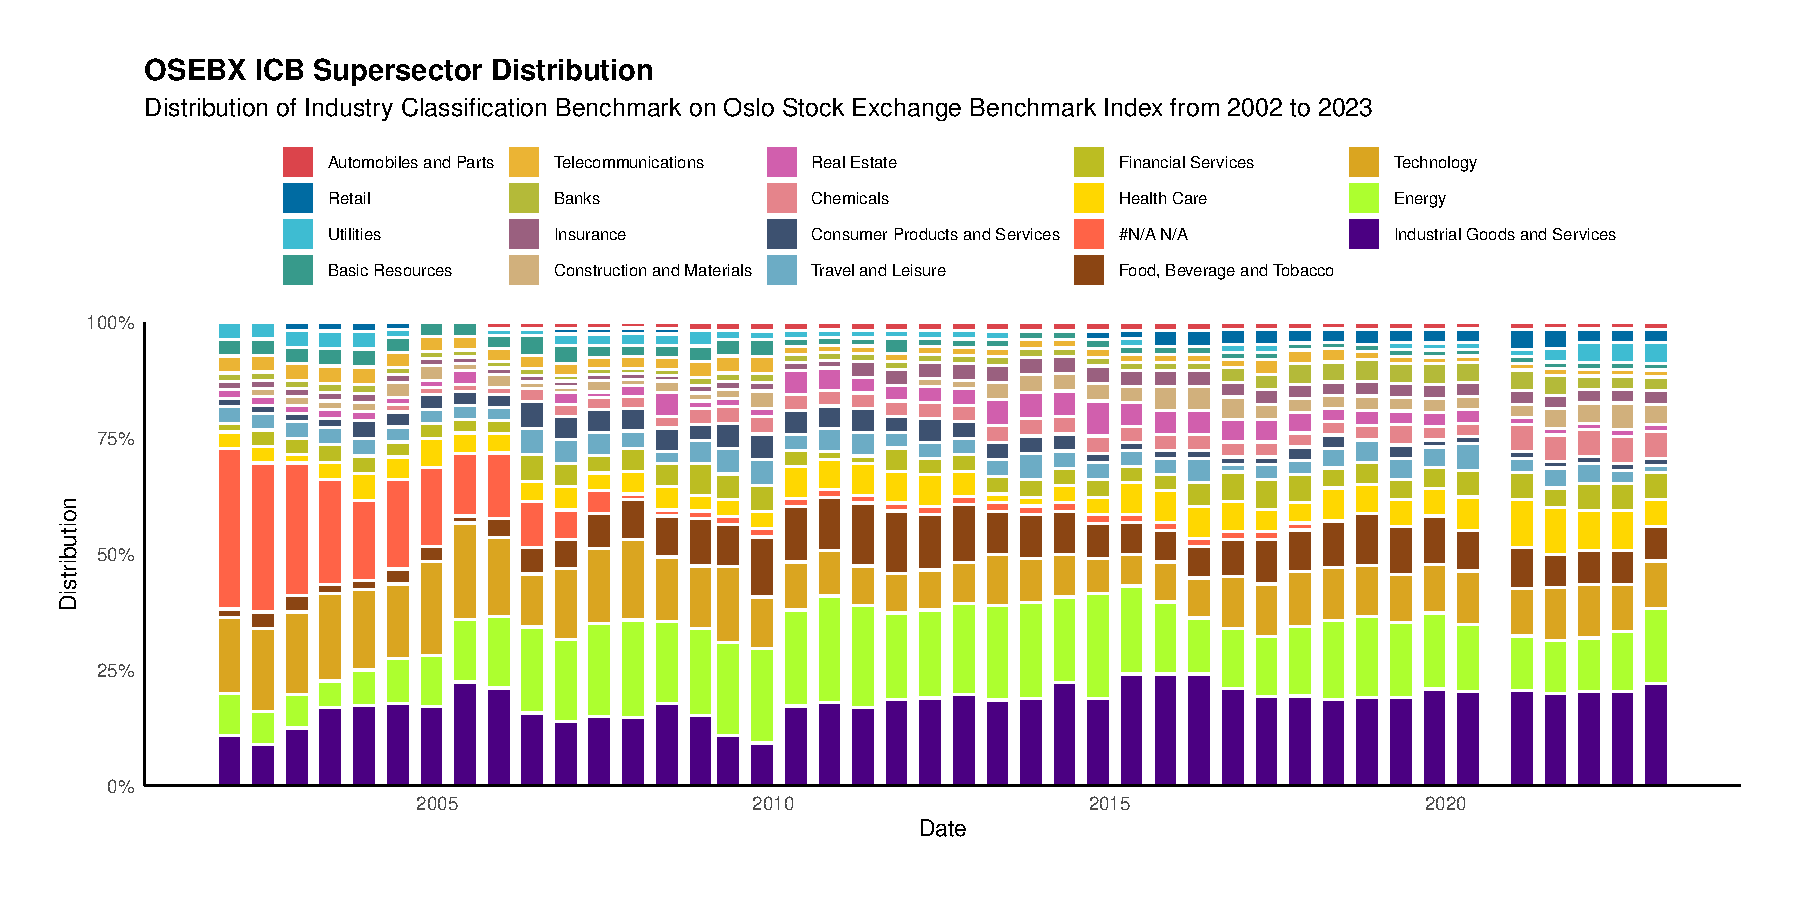
\includegraphics[width=\textwidth]{images/plot_sectors.pdf}
    \caption{{OSEBX ICB Supersector Distribution over Time}}
    \subcaption*{Industry classification benchmark (ICB) for companies on OSEBX in the period from 2002 to 2023. Notice that industry and energy companies dominate OSEBX.}
    \label{Oslo Stock Exchange Benchmark Index Sector Distribution}
\end{figure}